% !TeX spellcheck = en_GB 

\documentclass[a4paper, 12pt, oneside]{book}

\usepackage[english]{babel}
\usepackage[utf8]{inputenc}
\usepackage[pagestyles]{titlesec}
\usepackage{titletoc}
\usepackage{enumitem}
\usepackage{fancyhdr}
\usepackage[a4paper, margin = 2.5cm, headheight=14pt]{geometry}
\usepackage[hidelinks, colorlinks = false]{hyperref}
\usepackage[bottom]{footmisc}
\usepackage{bookmark}
\usepackage{fontspec}
\usepackage{graphicx}
\usepackage[labelfont = bf]{caption}
\usepackage{etoolbox}
\usepackage{tabularx}
\usepackage{colortbl}
\usepackage{float}

\usepackage[table]{xcolor}

\title{
	
\includegraphics[width=0.75\textwidth]{assets/logo.png}
	\\
	{\huge Hubbl, a gym bookings manager}
}
\author{Miquel de Domingo i Giralt}

\setmainfont{Inter}[BoldFont = Inter Bold]
\setmonofont[Scale=0.9]{JetBrains Mono}

\newfontfamily\semibf{Inter Semi Bold}

% Variable with the page that keeps the footer style
\def\footerstyle{- \fontsize{10pt}{10pt}\selectfont\thepage\ -}
\pagestyle{fancy}
% Remove the horizontal bar from the header
\renewcommand{\headrulewidth}{0pt}
% Clear everythihg
\fancyhf{}
% Set header style
\rhead{\small\textit{\nouppercase{\rightmark}}}
% Set the footer page number
\fancyfoot[C]{\footerstyle}
% Update the footer in chapter and other plain views
\fancypagestyle{plain}{%
    \renewcommand{\headrulewidth}{0pt}%
    \fancyhf{}%
    \fancyfoot[C]{\footerstyle}%
}

\setlength\parindent{0pt}
\setcounter{secnumdepth}{5}
\setcounter{tocdepth}{5}

% Tables format
\definecolor{rowColor}{RGB}{242, 242, 242}
\renewcommand{\arraystretch}{1.5}

\titleformat{\chapter}[hang]{\normalfont\huge\bfseries}{\thechapter. }{4pt}{\Huge}
\titlespacing{\chapter}{0pt}{-32pt}{12pt}

\begin{document}
\frontmatter
\maketitle
\listoffigures
\mainmatter
\chapter{Implementation and results}
\section{Results}
There are some views that did not fit in the screen, therefore two images have been made. Furthermore, most of the create and update actions are performed inside a modal or a dialog. Instead of adding two screenshots with the same content, only with small text changed, only the create dialog has been attached. Furthermore, the zoom applied is of 90\%, allowing more content to be displayed in the screenshot.
\subsection{Core application}
In order to reduce the amount of screenshots that are added, the screenshots have been made when a user is logged as an owner. A worker's is nearly as the worker's one, just with some actions not allowed, depending on their permissions.
\subsubsection{Authentication}
\begin{figure}[H]
	\centering
	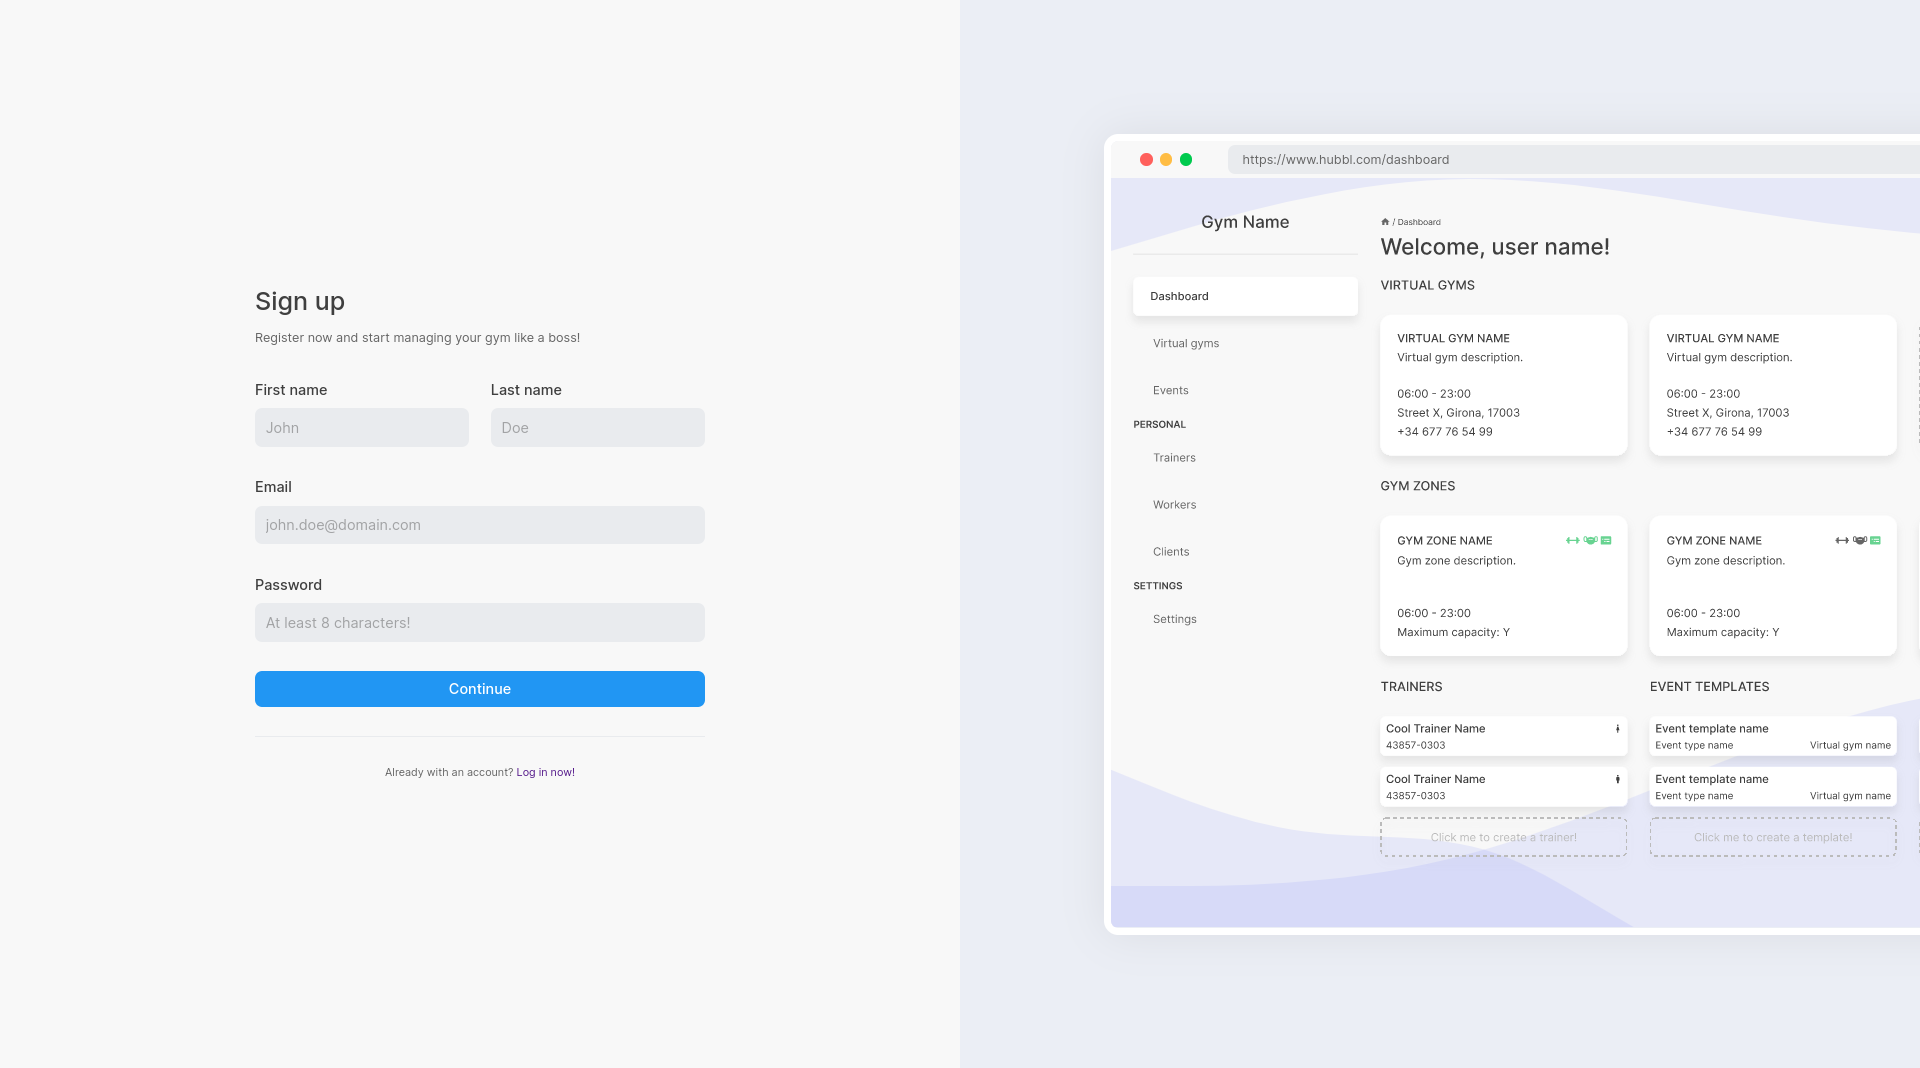
\includegraphics[width=\textwidth]{assets/core-screenshots/sign-up-one.png}
	\caption{Step one of the sign up process}
\end{figure}
\begin{figure}[H]
	\centering
	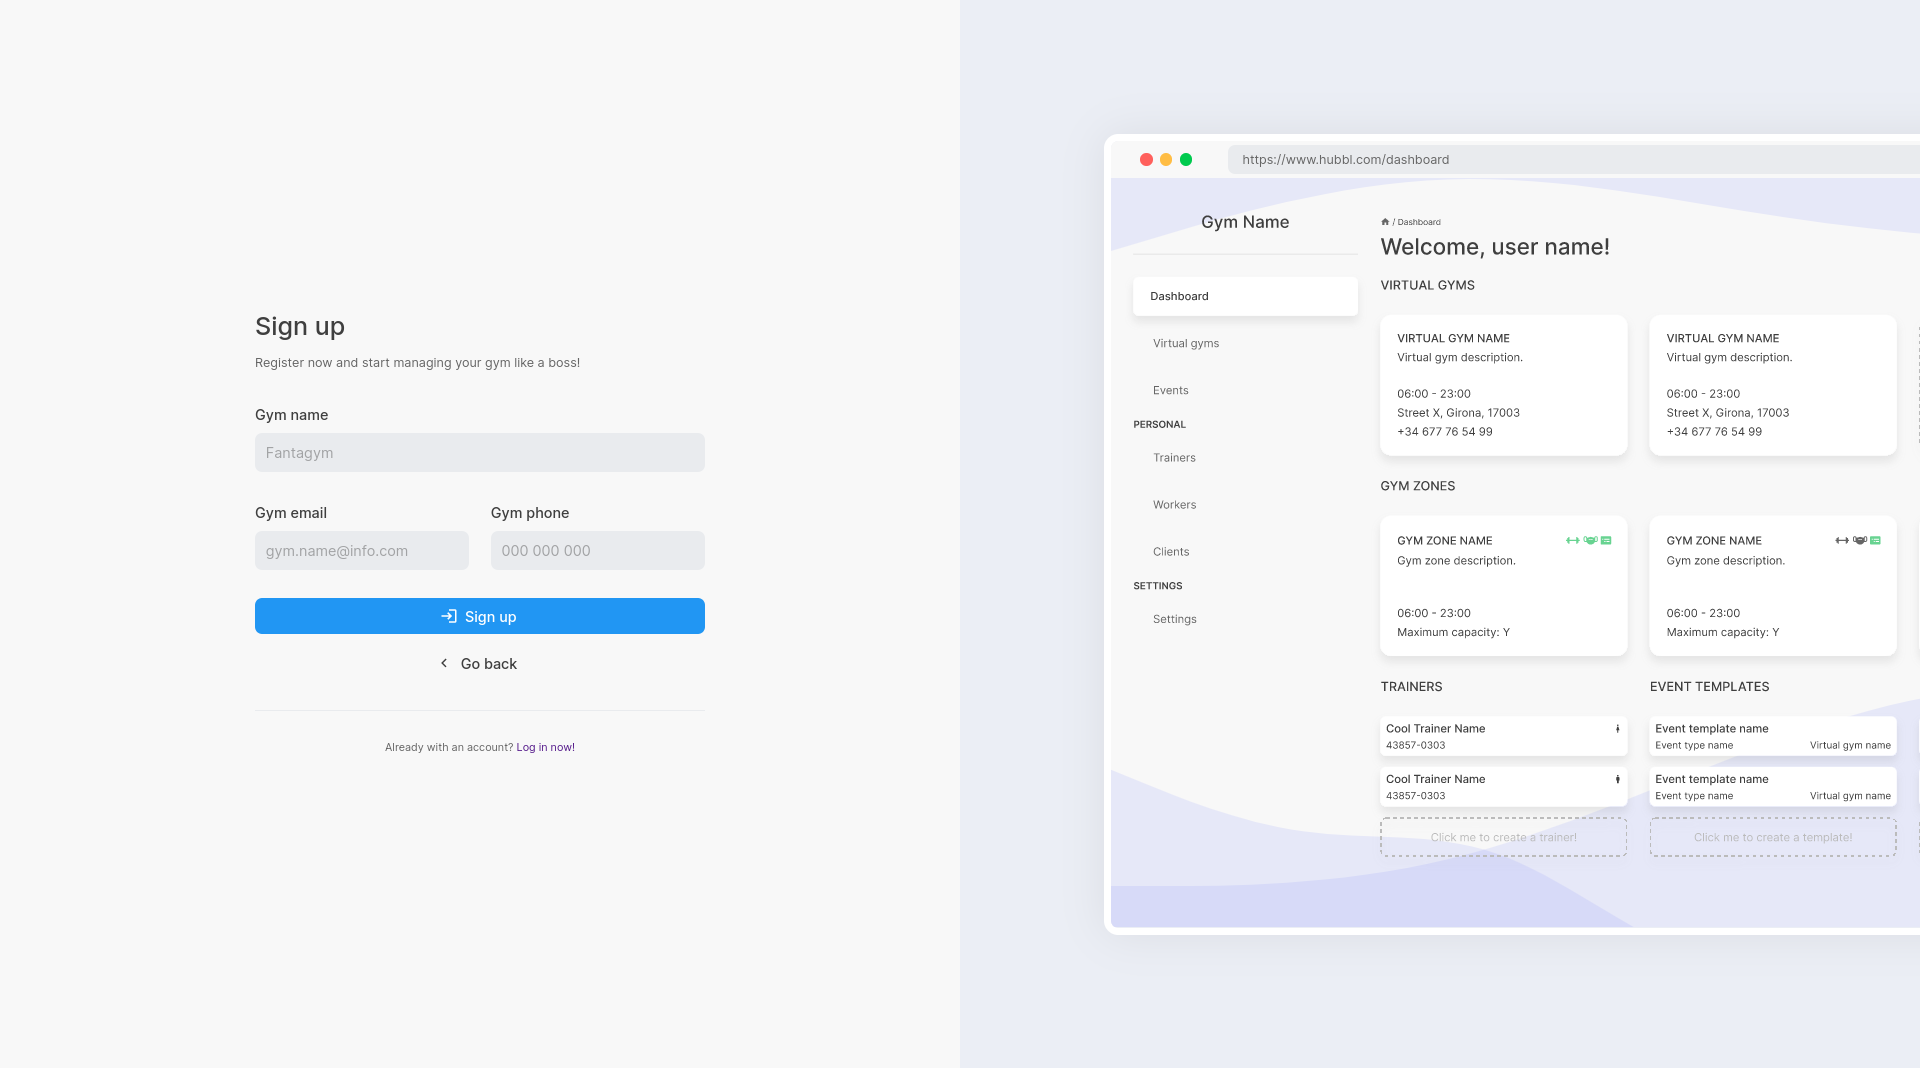
\includegraphics[width=\textwidth]{assets/core-screenshots/sign-up-two.png}
	\caption{Step two of the sign up process}
\end{figure}
\begin{figure}[H]
	\centering
	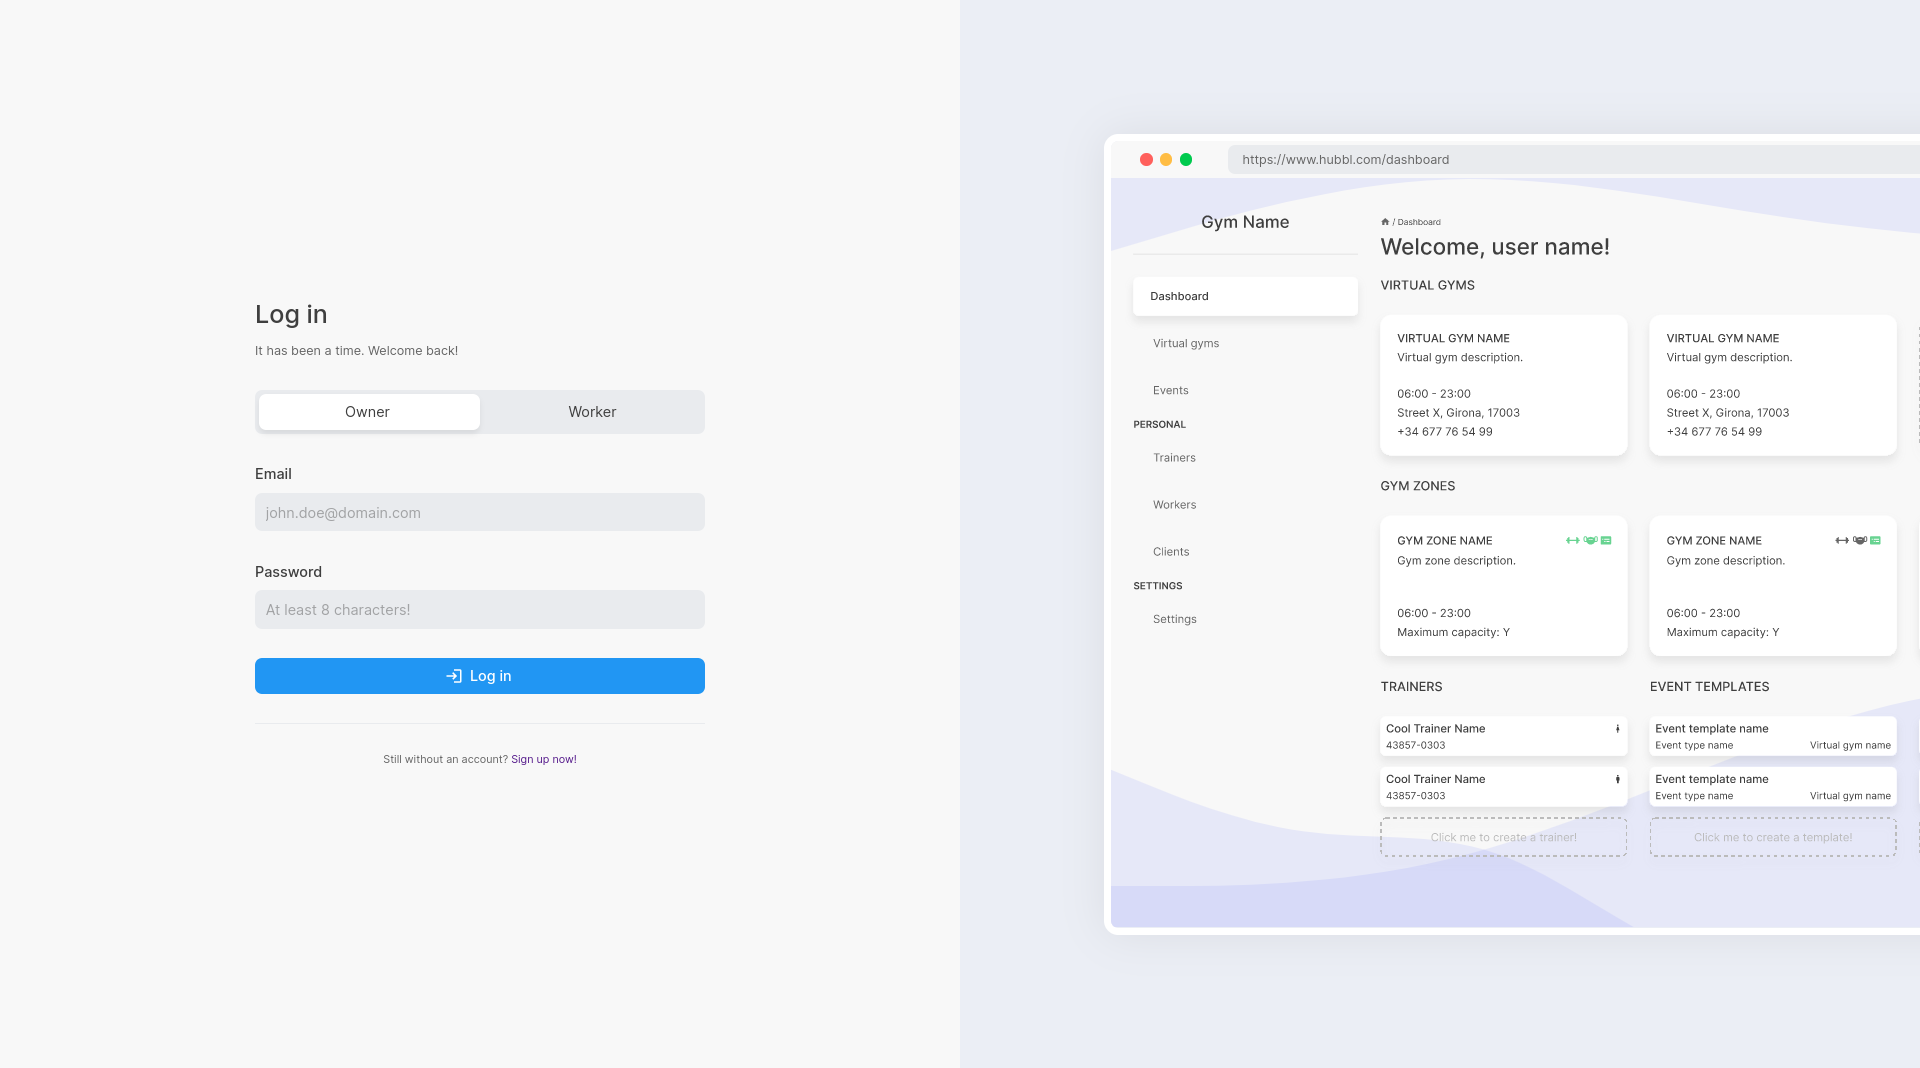
\includegraphics[width=\textwidth]{assets/core-screenshots/log-in.png}
	\caption{Log in page}
\end{figure}
\subsubsection{Dashboard page}
\begin{figure}[H]
	\centering
	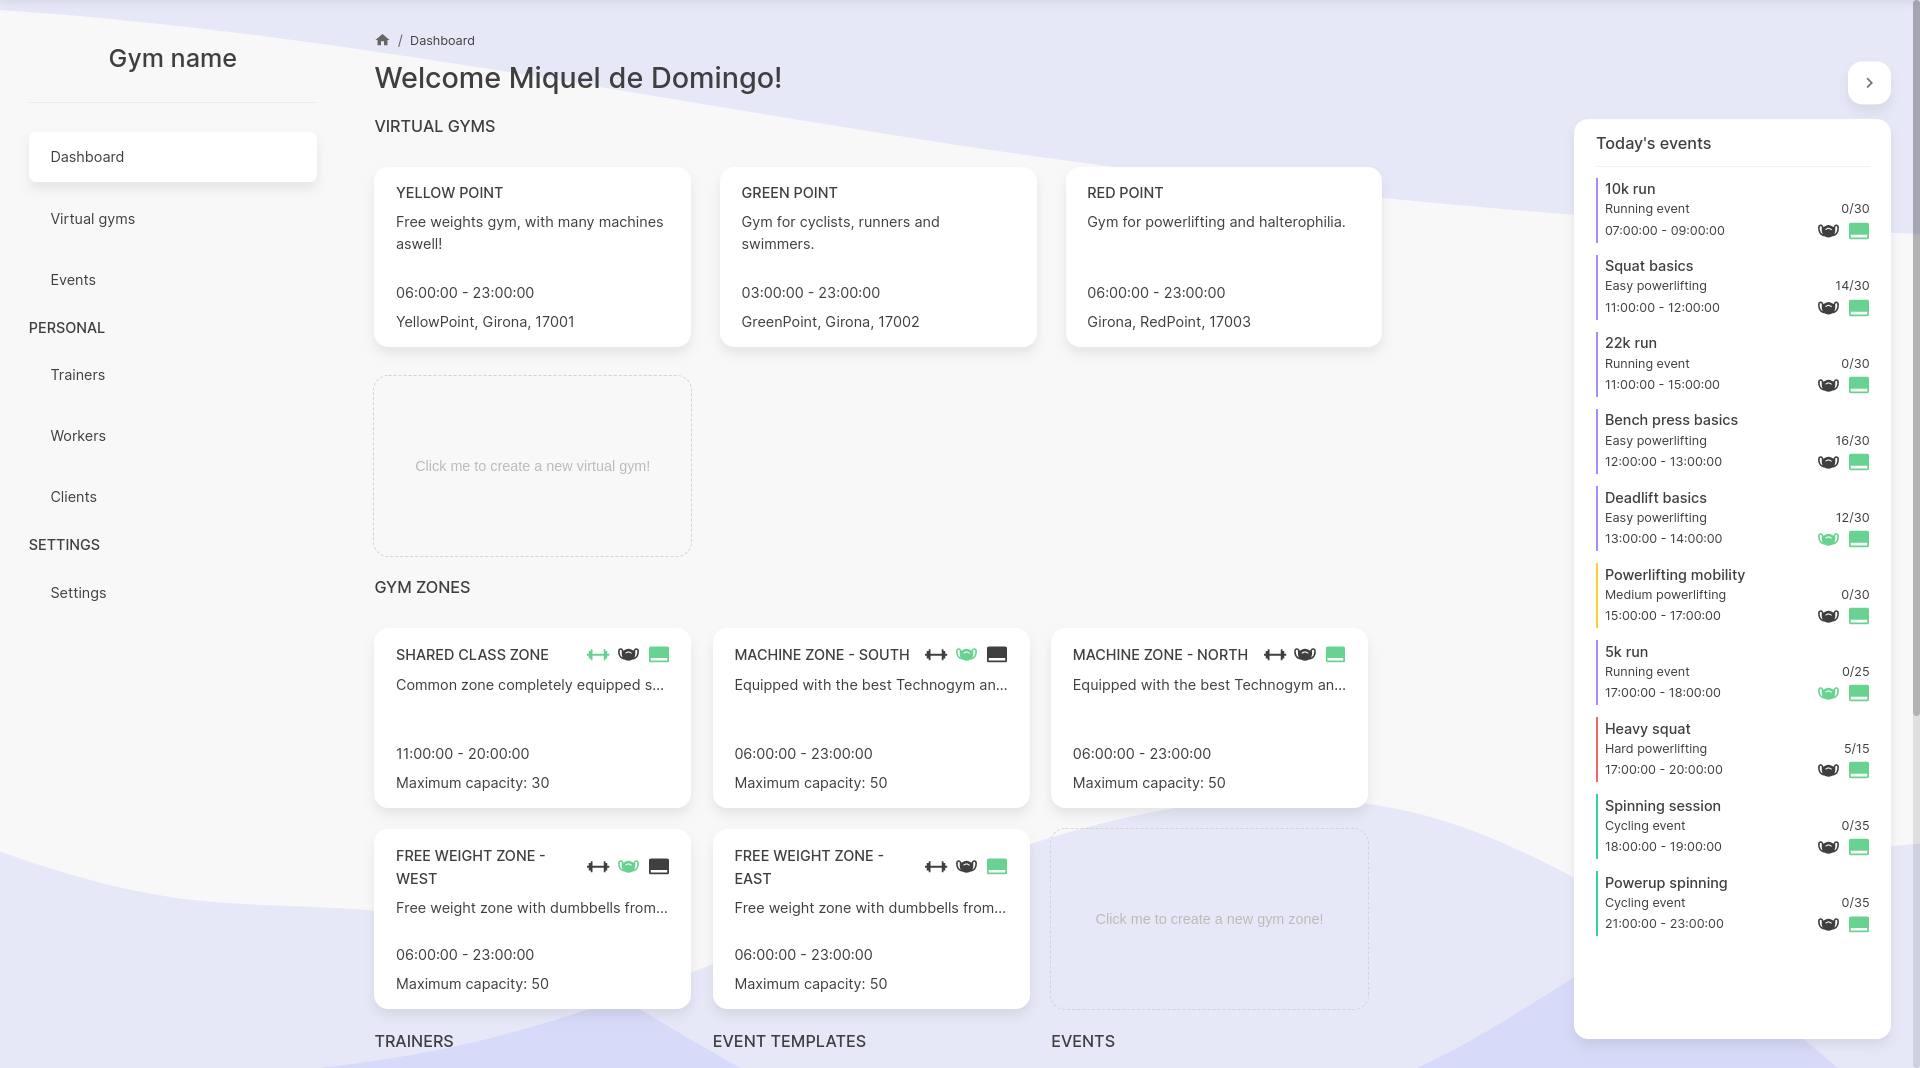
\includegraphics[width=\textwidth]{assets/core-screenshots/dashboard-one.png}
	\caption{First screenshot of the dashboard page}
\end{figure}
\begin{figure}[H]
	\centering
	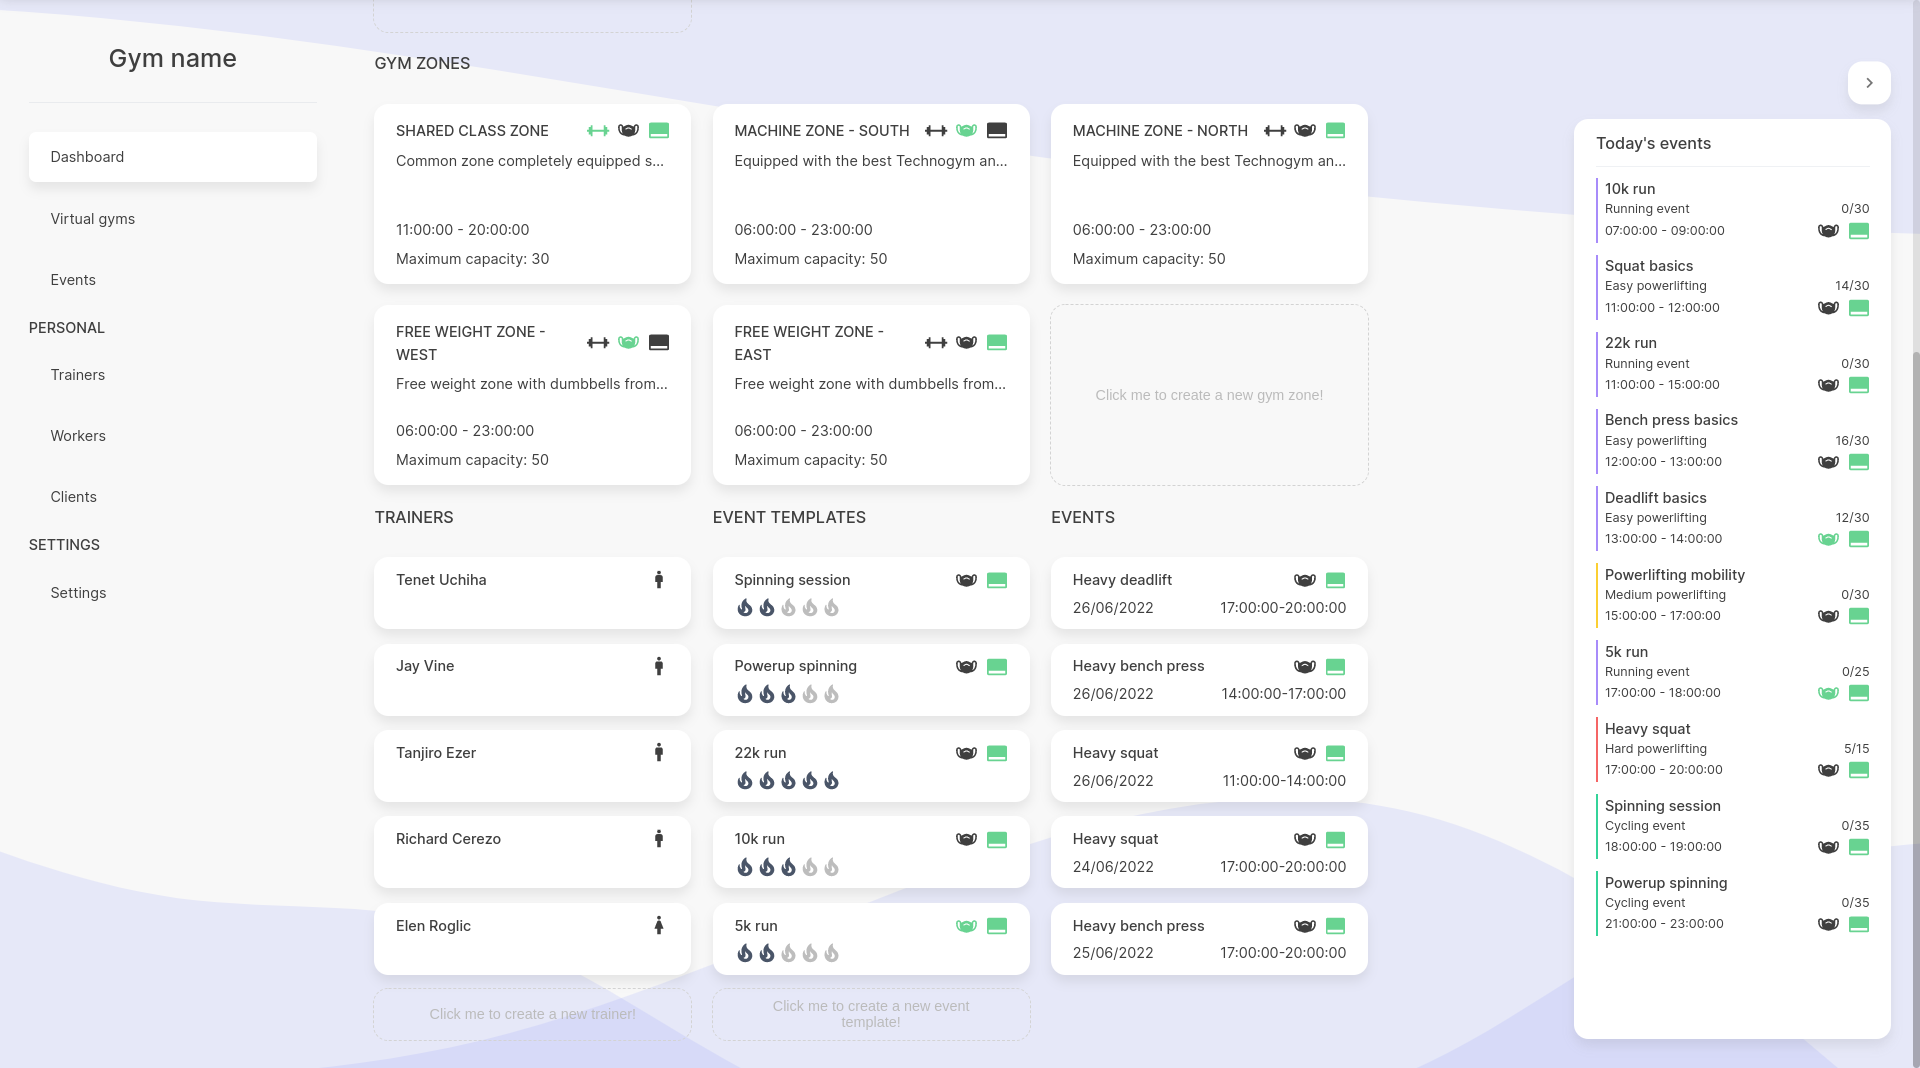
\includegraphics[width=\textwidth]{assets/core-screenshots/dashboard-two.png}
	\caption{Second screenshot of the dashboard page}
\end{figure}
\subsubsection{Virtual gyms}
\begin{figure}[H]
	\centering
	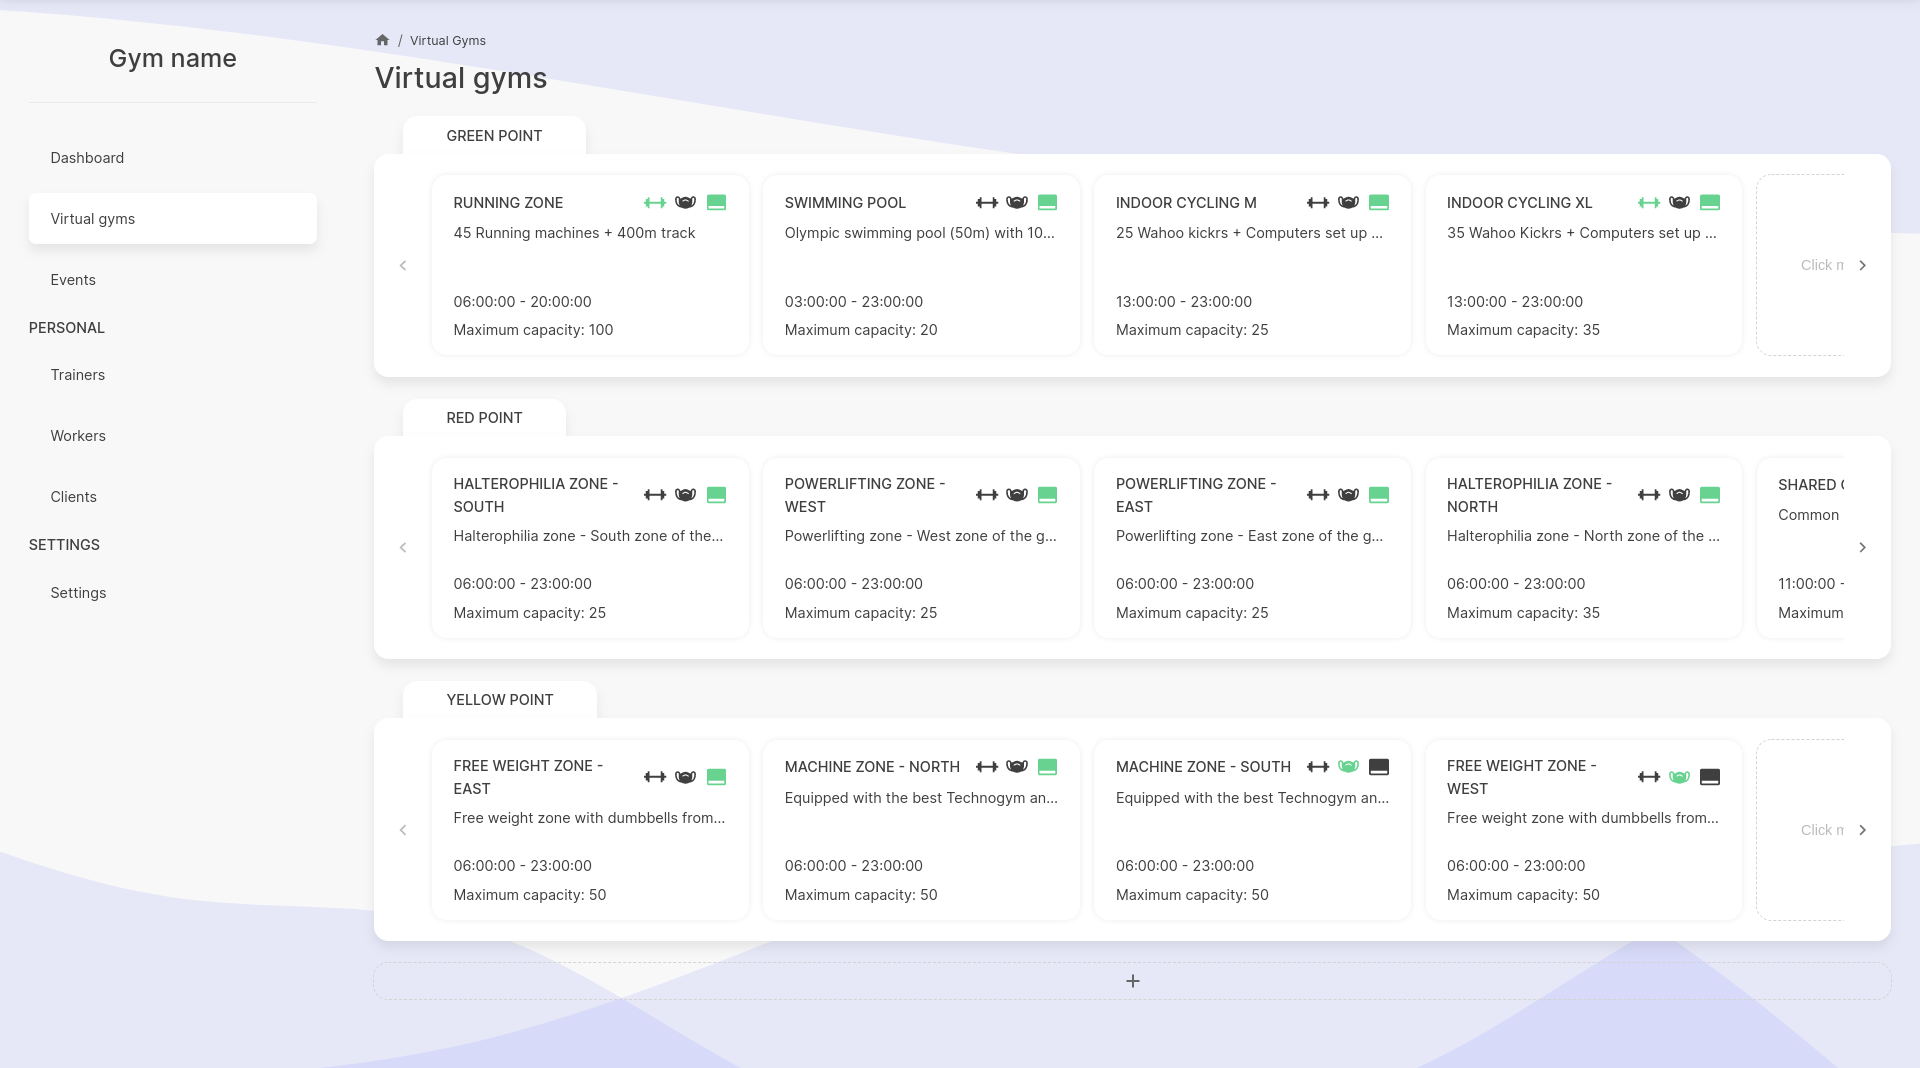
\includegraphics[width=\textwidth]{assets/core-screenshots/virtual-gyms.png}
	\caption{Virtual gyms page}
\end{figure}
Whenever a virtual gym has been clicked (by clicking at its name), the user is redirected to the above page, which displays all the gym zones of the chosen virtual gym.
\begin{figure}[H]
	\centering
	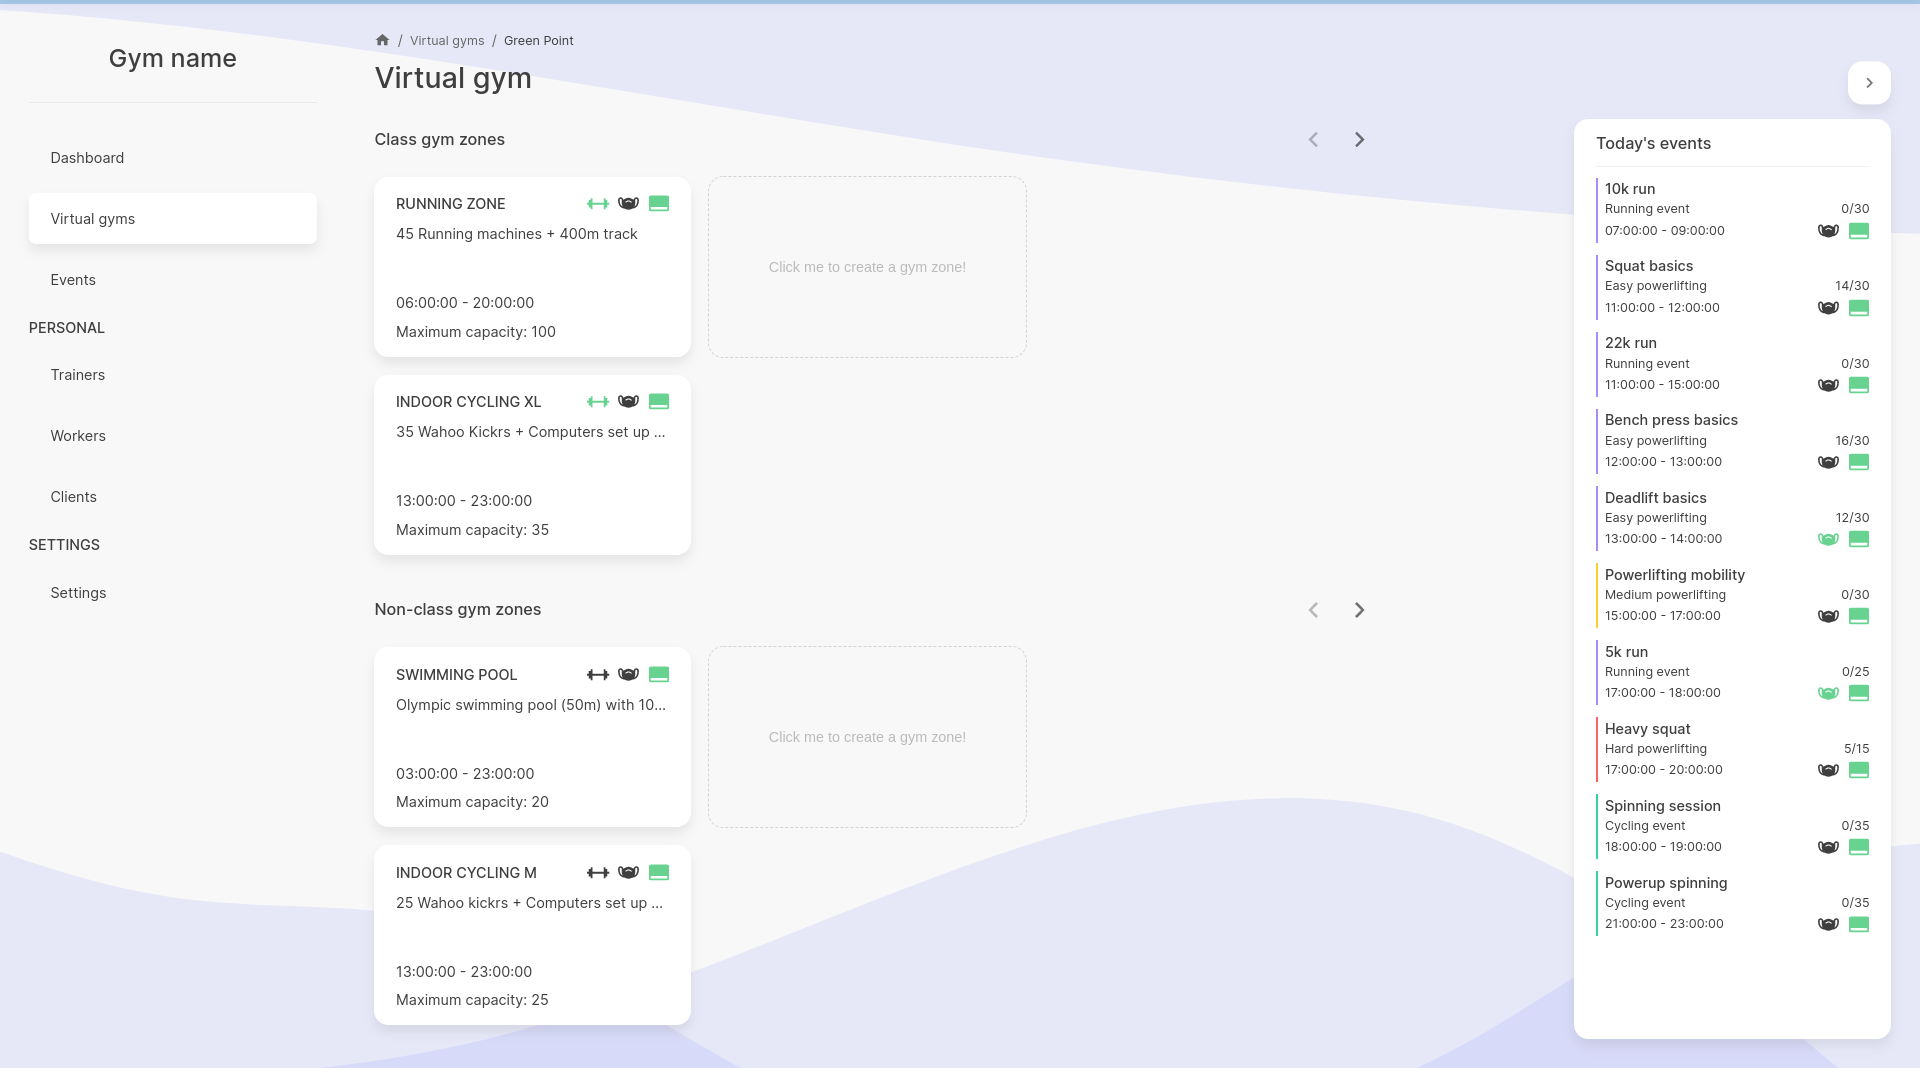
\includegraphics[width=\textwidth]{assets/core-screenshots/virtual-gym.png}
	\caption{Virtual gym page}
\end{figure}
\begin{figure}[H]
	\centering
	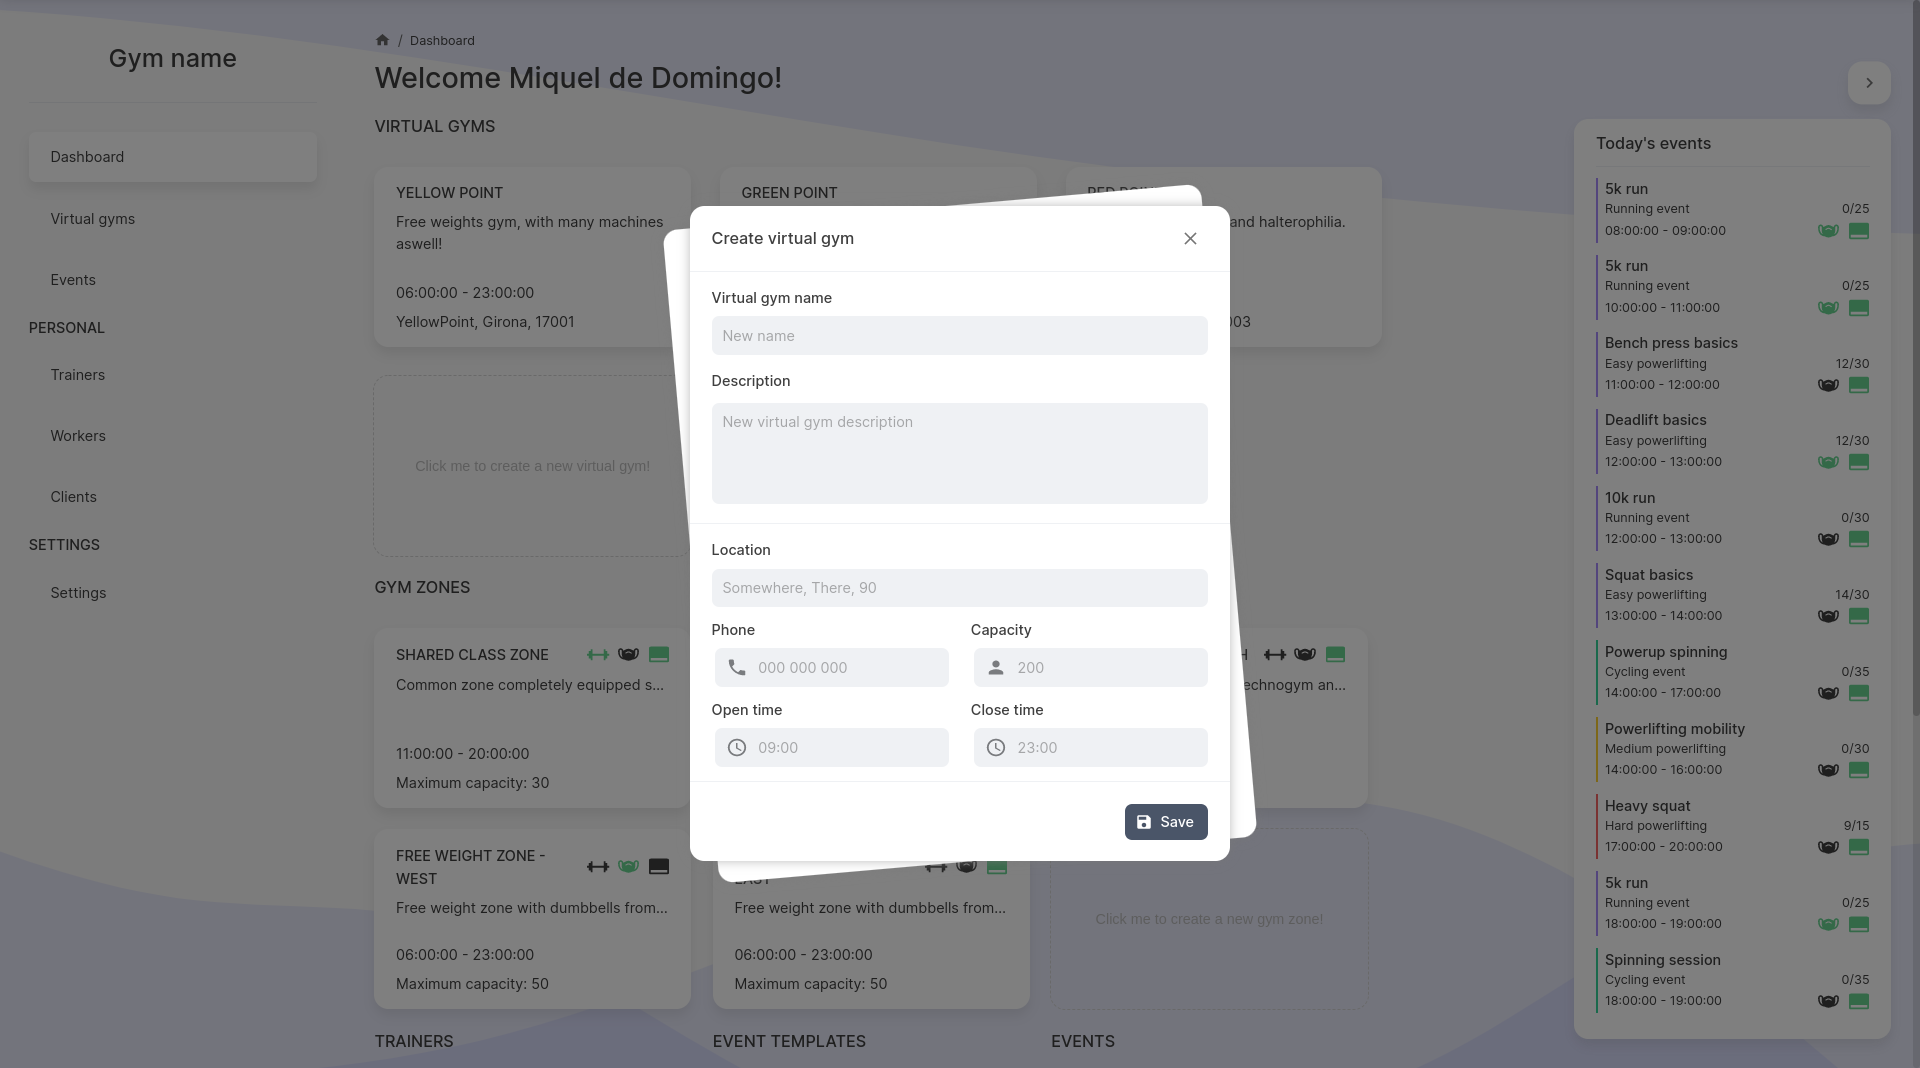
\includegraphics[width=\textwidth]{assets/core-screenshots/create-virtual-gym.png}
	\caption{Creation of a virtual gym}
\end{figure}
\subsubsection{Gym zone}
This view is only limited to the class type gym zones. That is becasue the non-class type do not have an events calendar.
\begin{figure}[H]
	\centering
	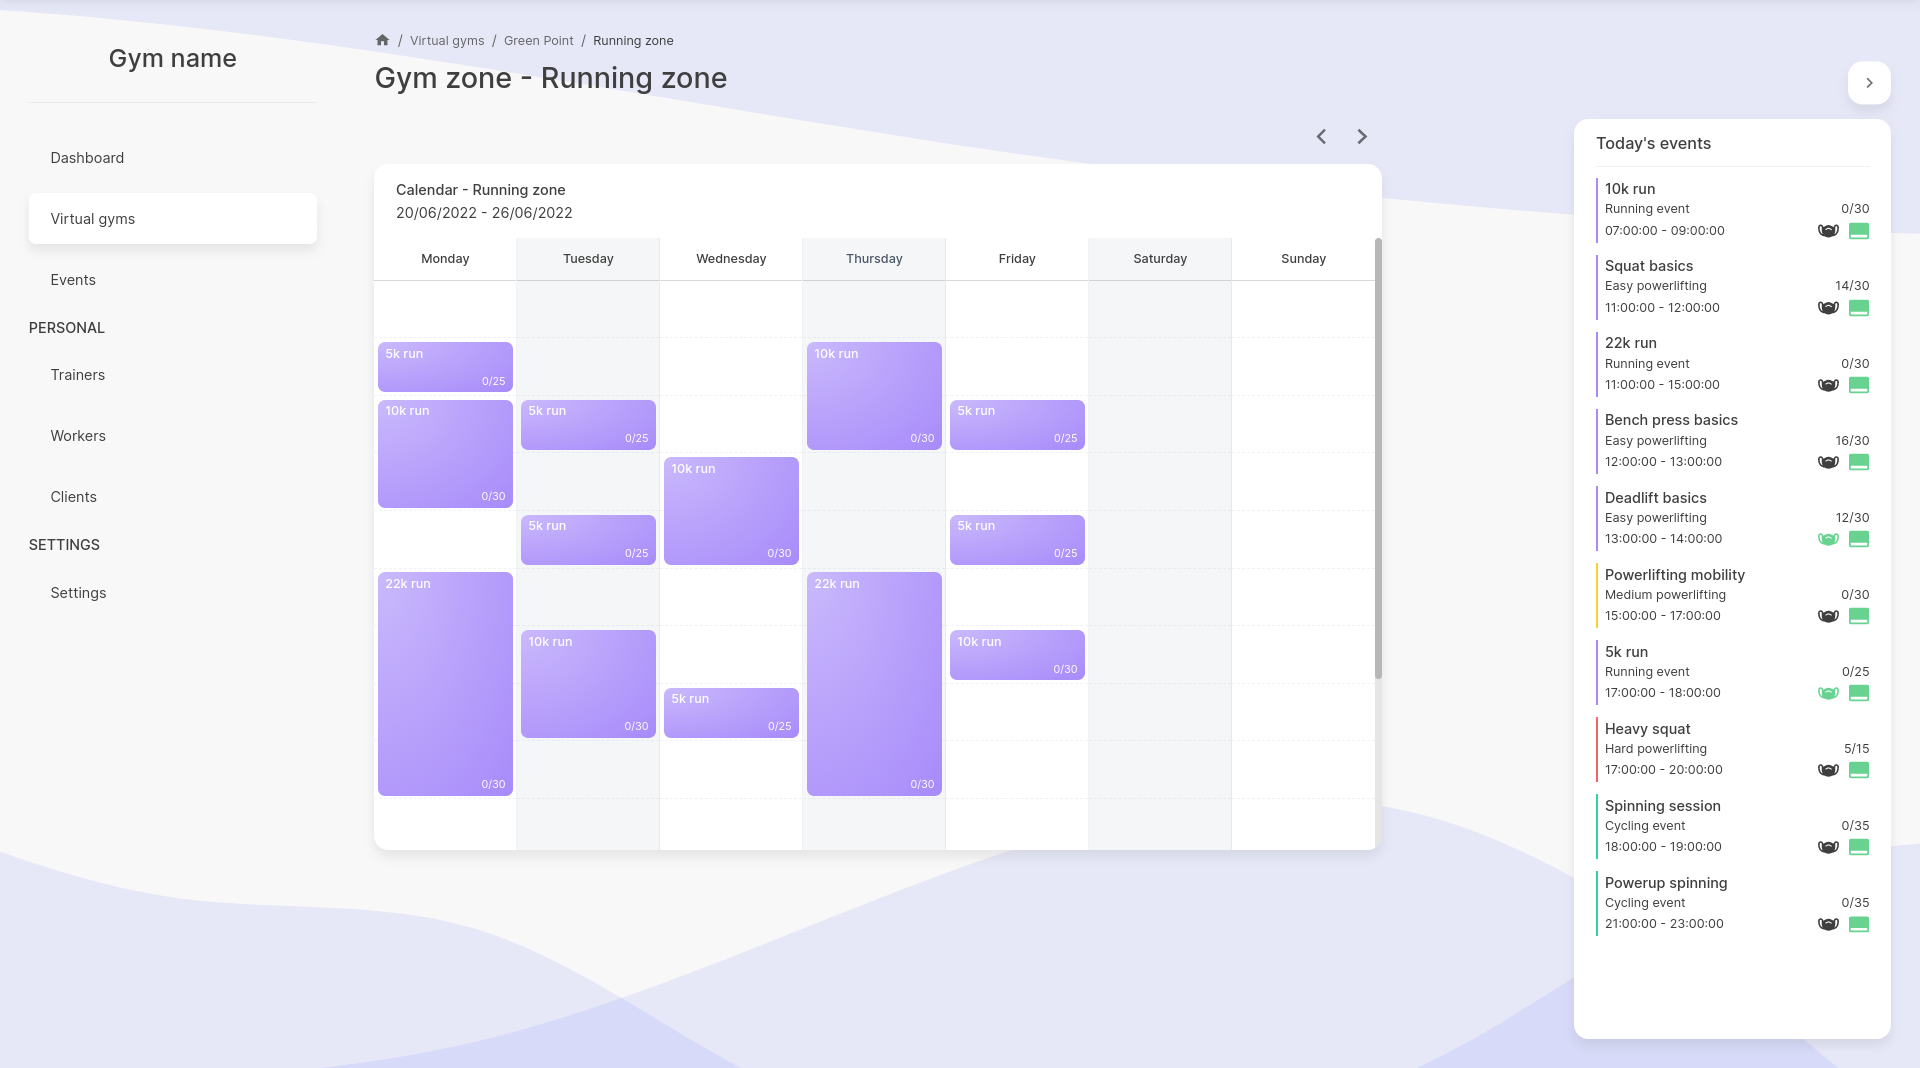
\includegraphics[width=\textwidth]{assets/core-screenshots/gym-zone-one.png}
	\caption{View of a calendar with events of the same event type}
\end{figure}
\begin{figure}[H]
	\centering
	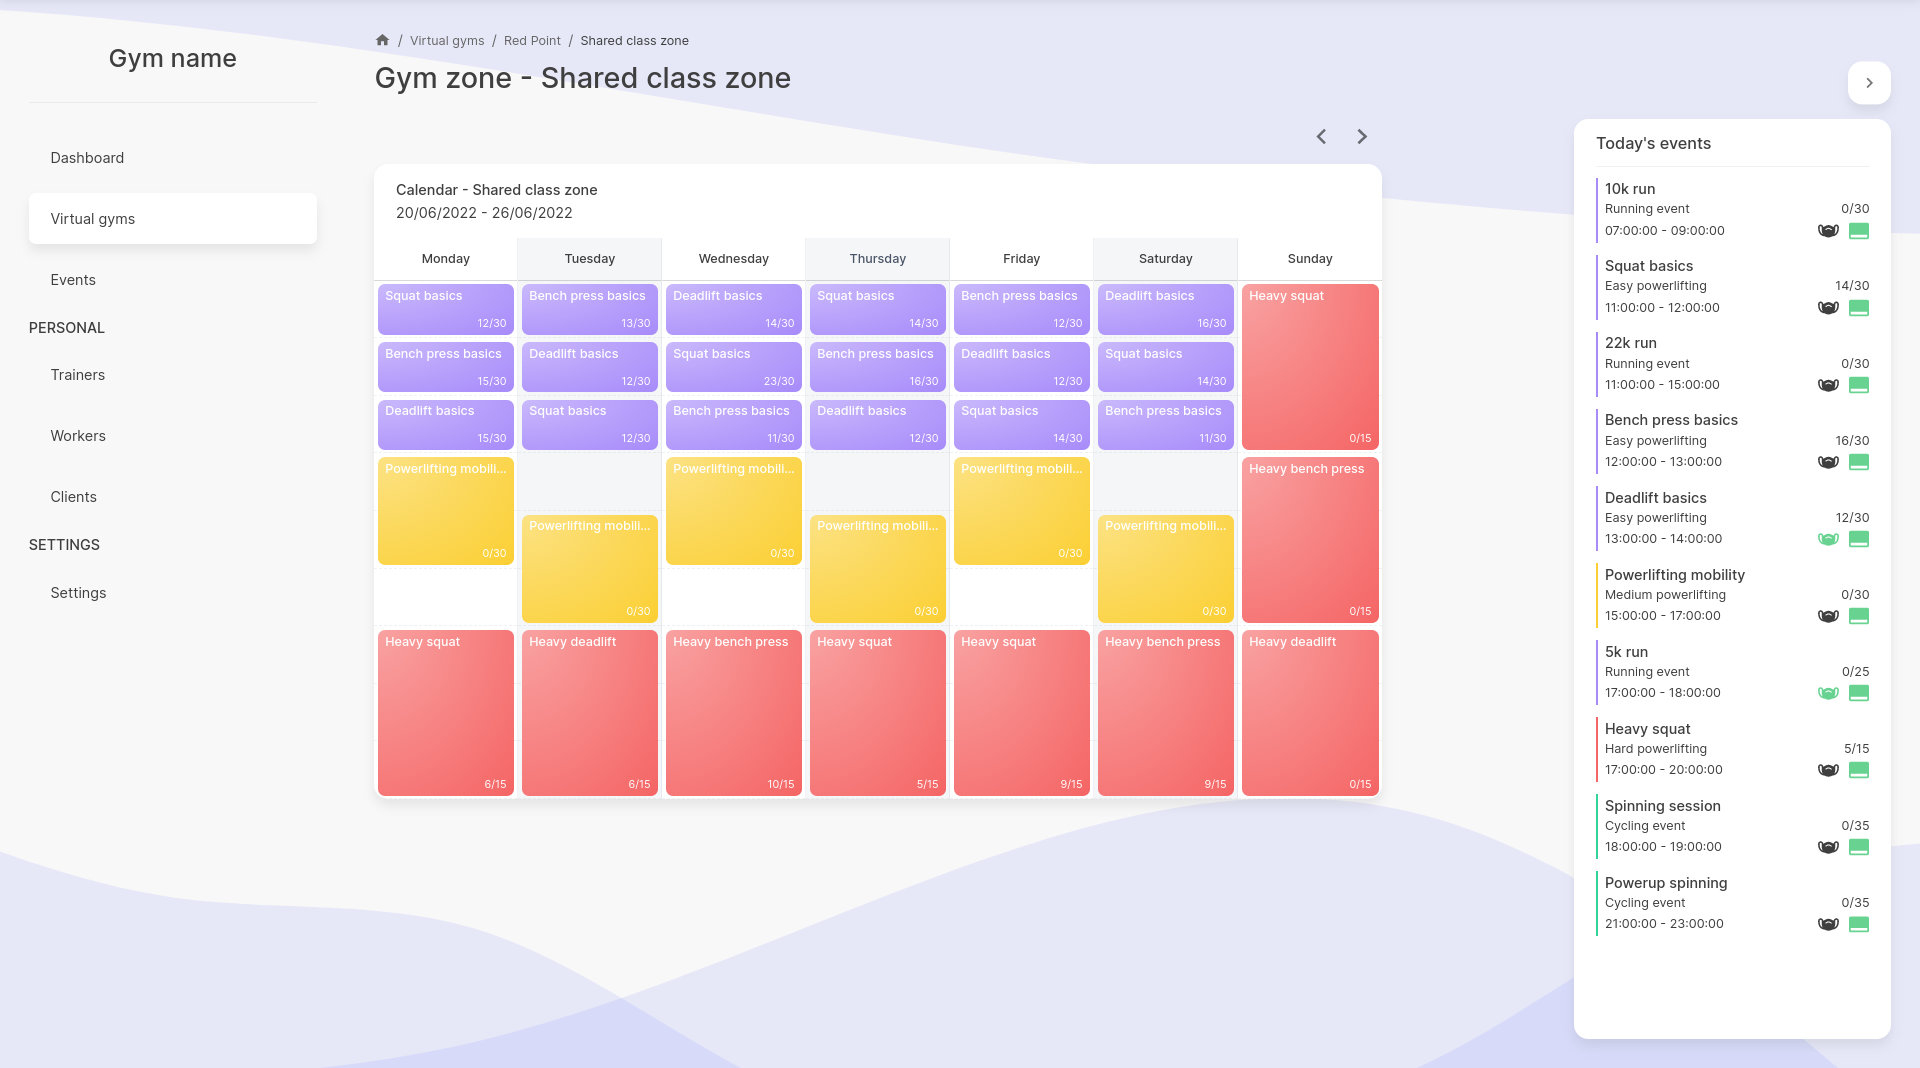
\includegraphics[width=\textwidth]{assets/core-screenshots/gym-zone-two.png}
	\caption{View of a calendar with events of different event type}
\end{figure}
Gym zones can be created from different views, which are the dashboard, the virtual gyms list page and the single virtual gym's page.
\begin{figure}[H]
	\centering
	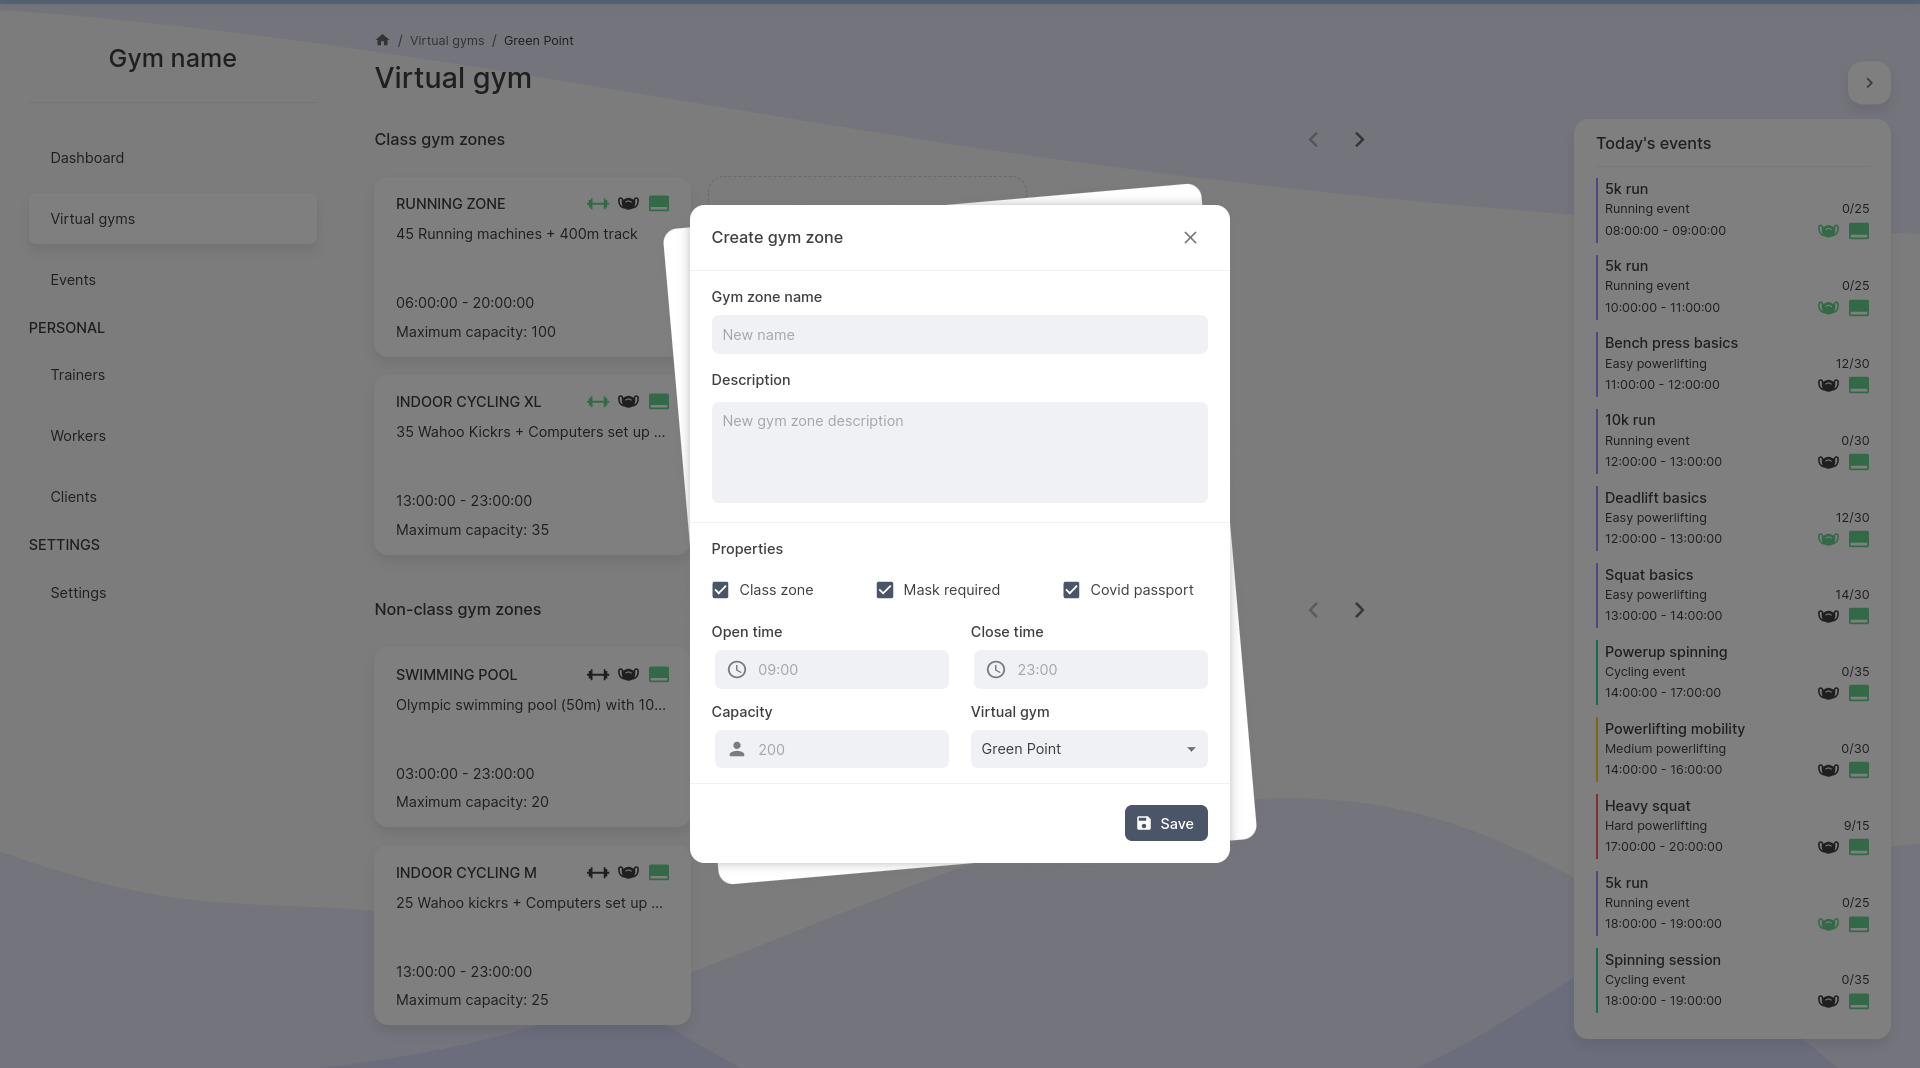
\includegraphics[width=\textwidth]{assets/core-screenshots/create-gym-zone.png}
	\caption{Virtual gym page}
\end{figure}
\begin{figure}[H]
	\centering
	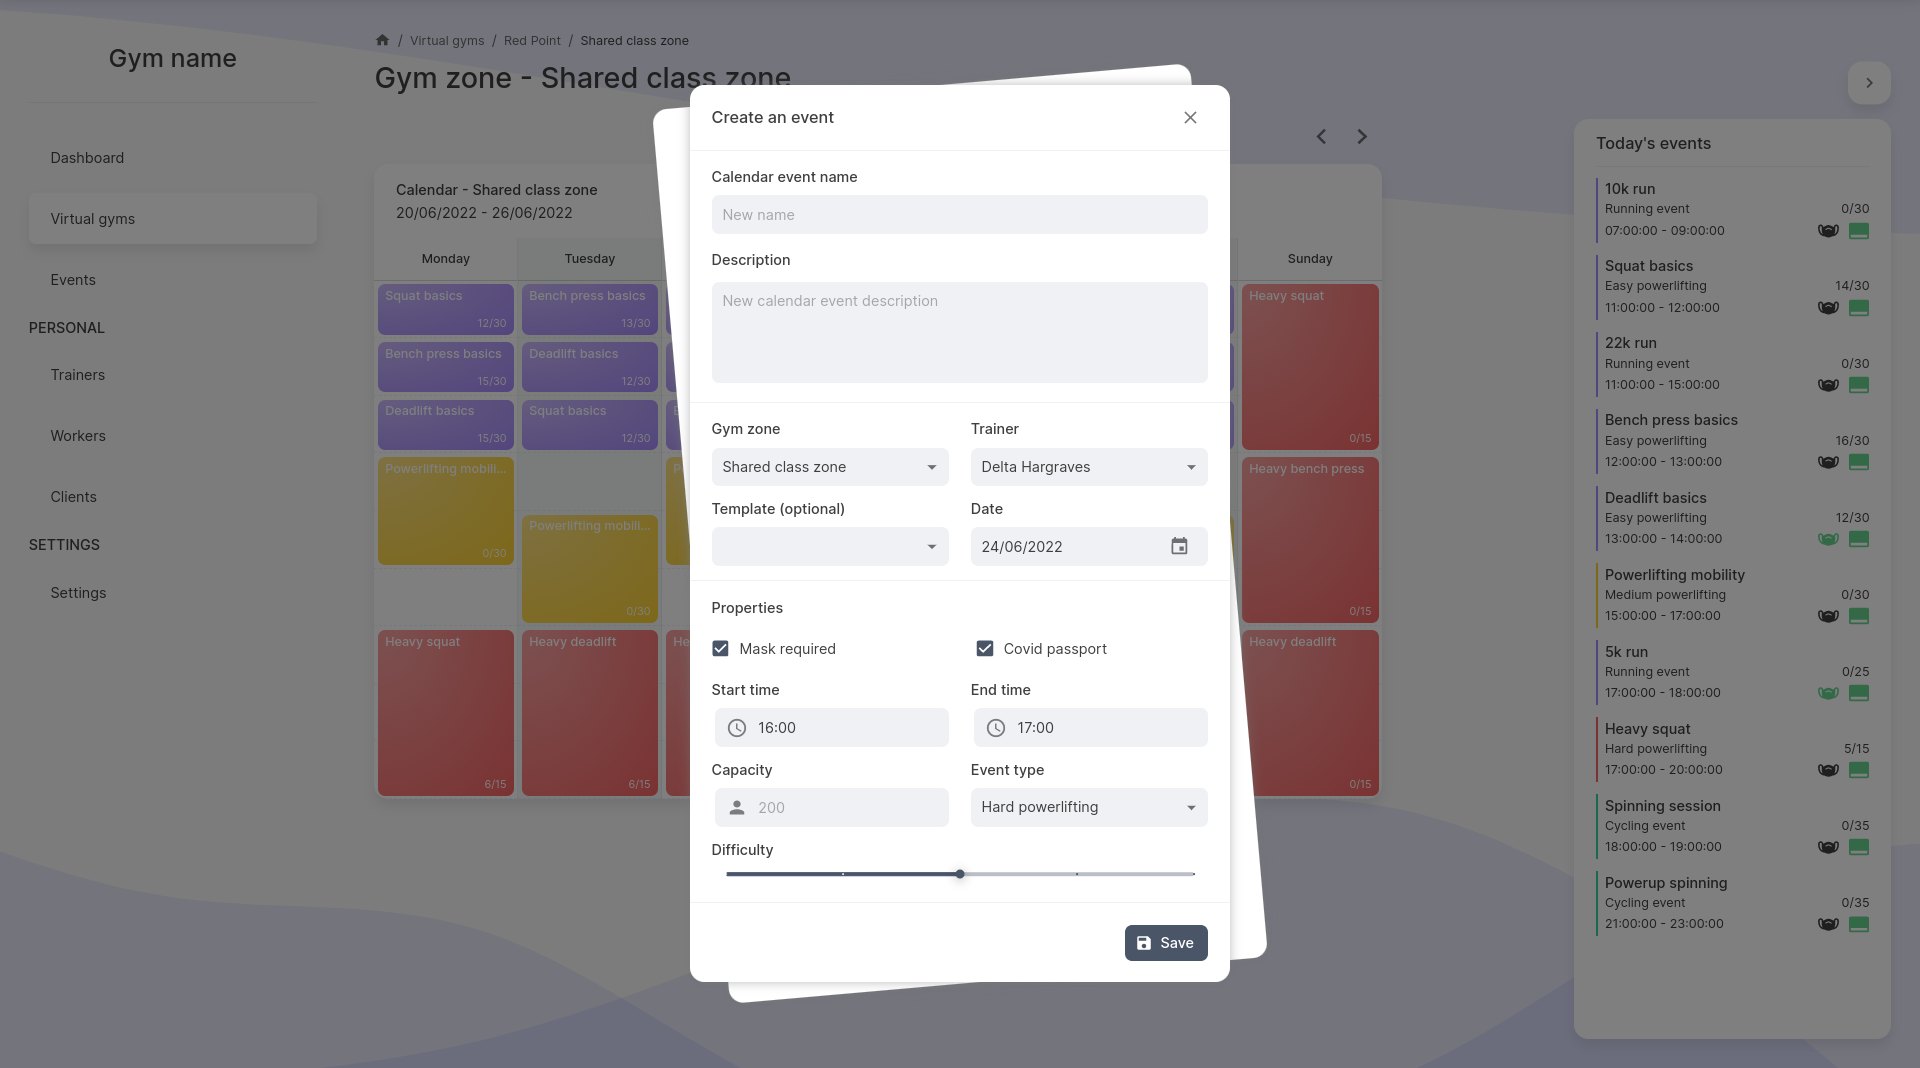
\includegraphics[width=\textwidth]{assets/core-screenshots/create-event.png}
	\caption{Creation of an event for a calendar}
\end{figure}
\subsubsection{Events}
\begin{figure}[H]
	\centering
	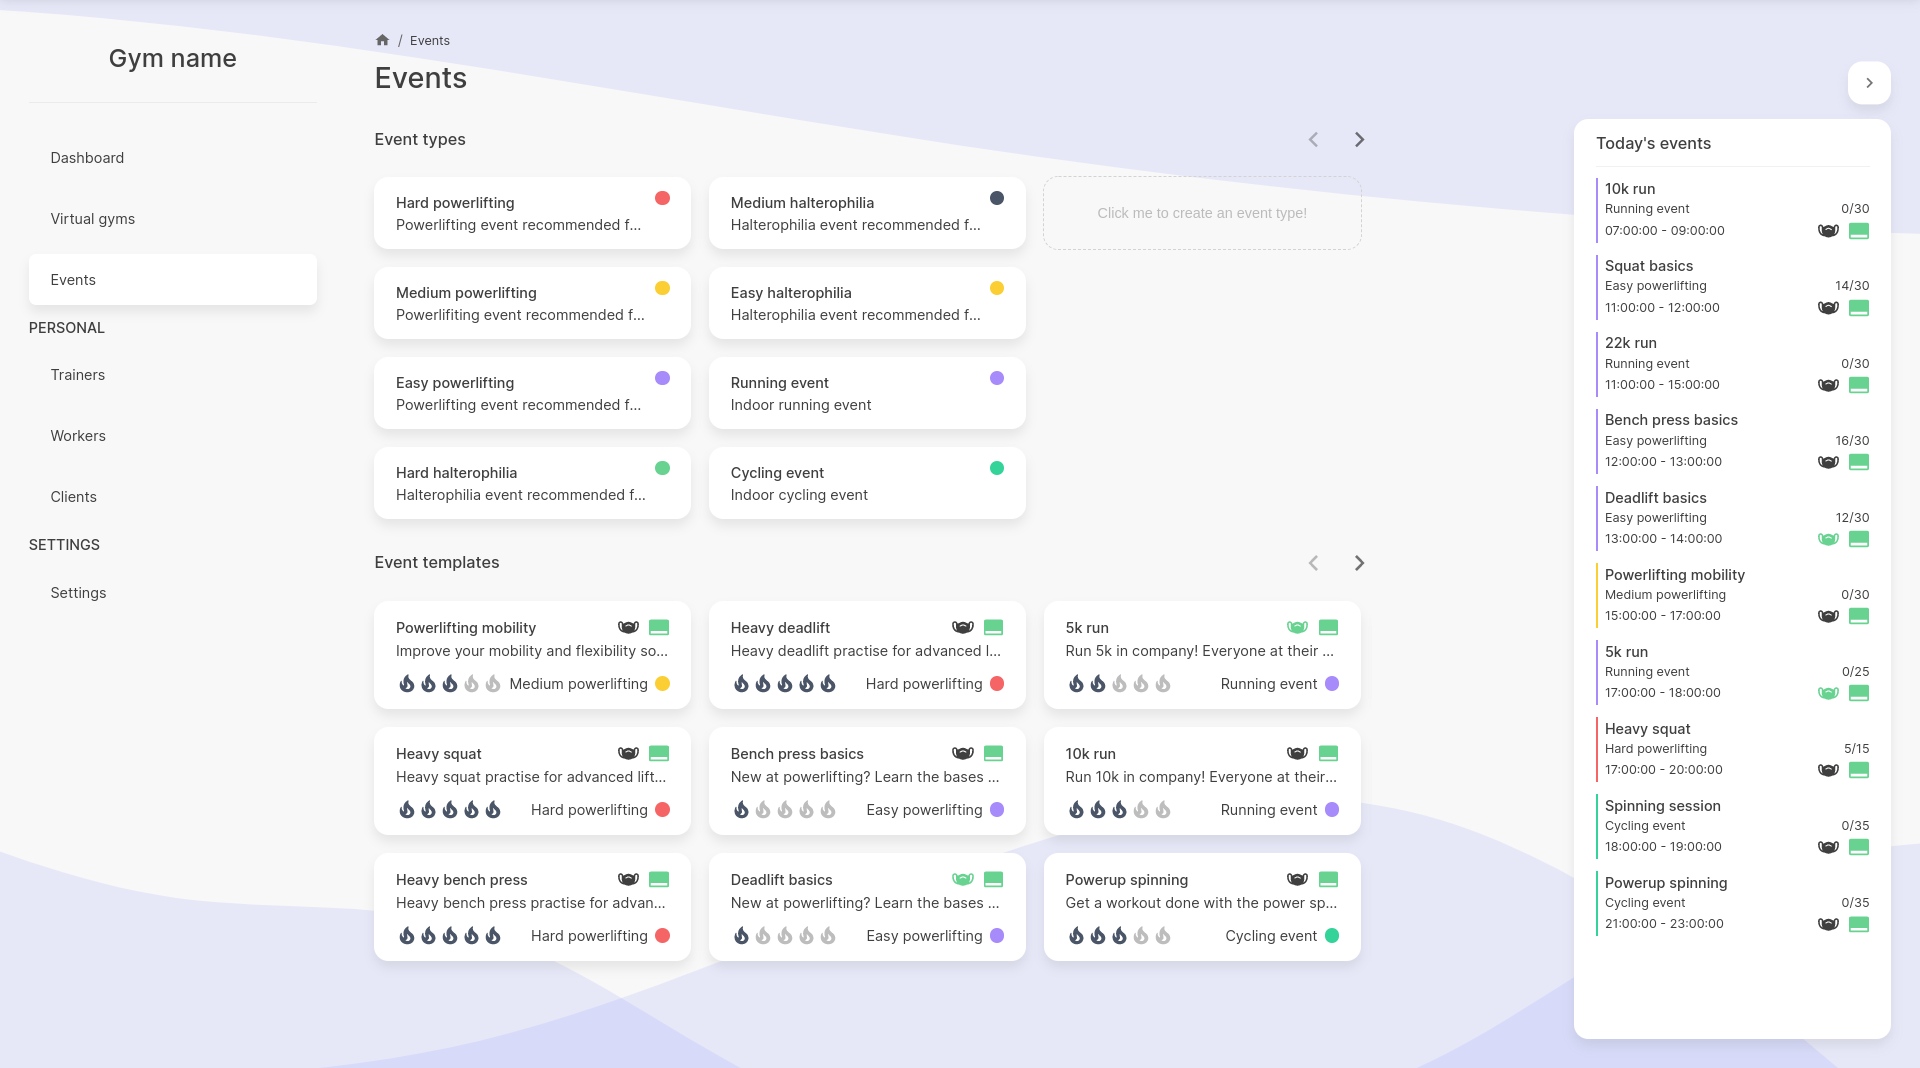
\includegraphics[width=\textwidth]{assets/core-screenshots/events.png}
	\caption{Events page with event types and event templates}
\end{figure}
\begin{figure}[H]
	\centering
	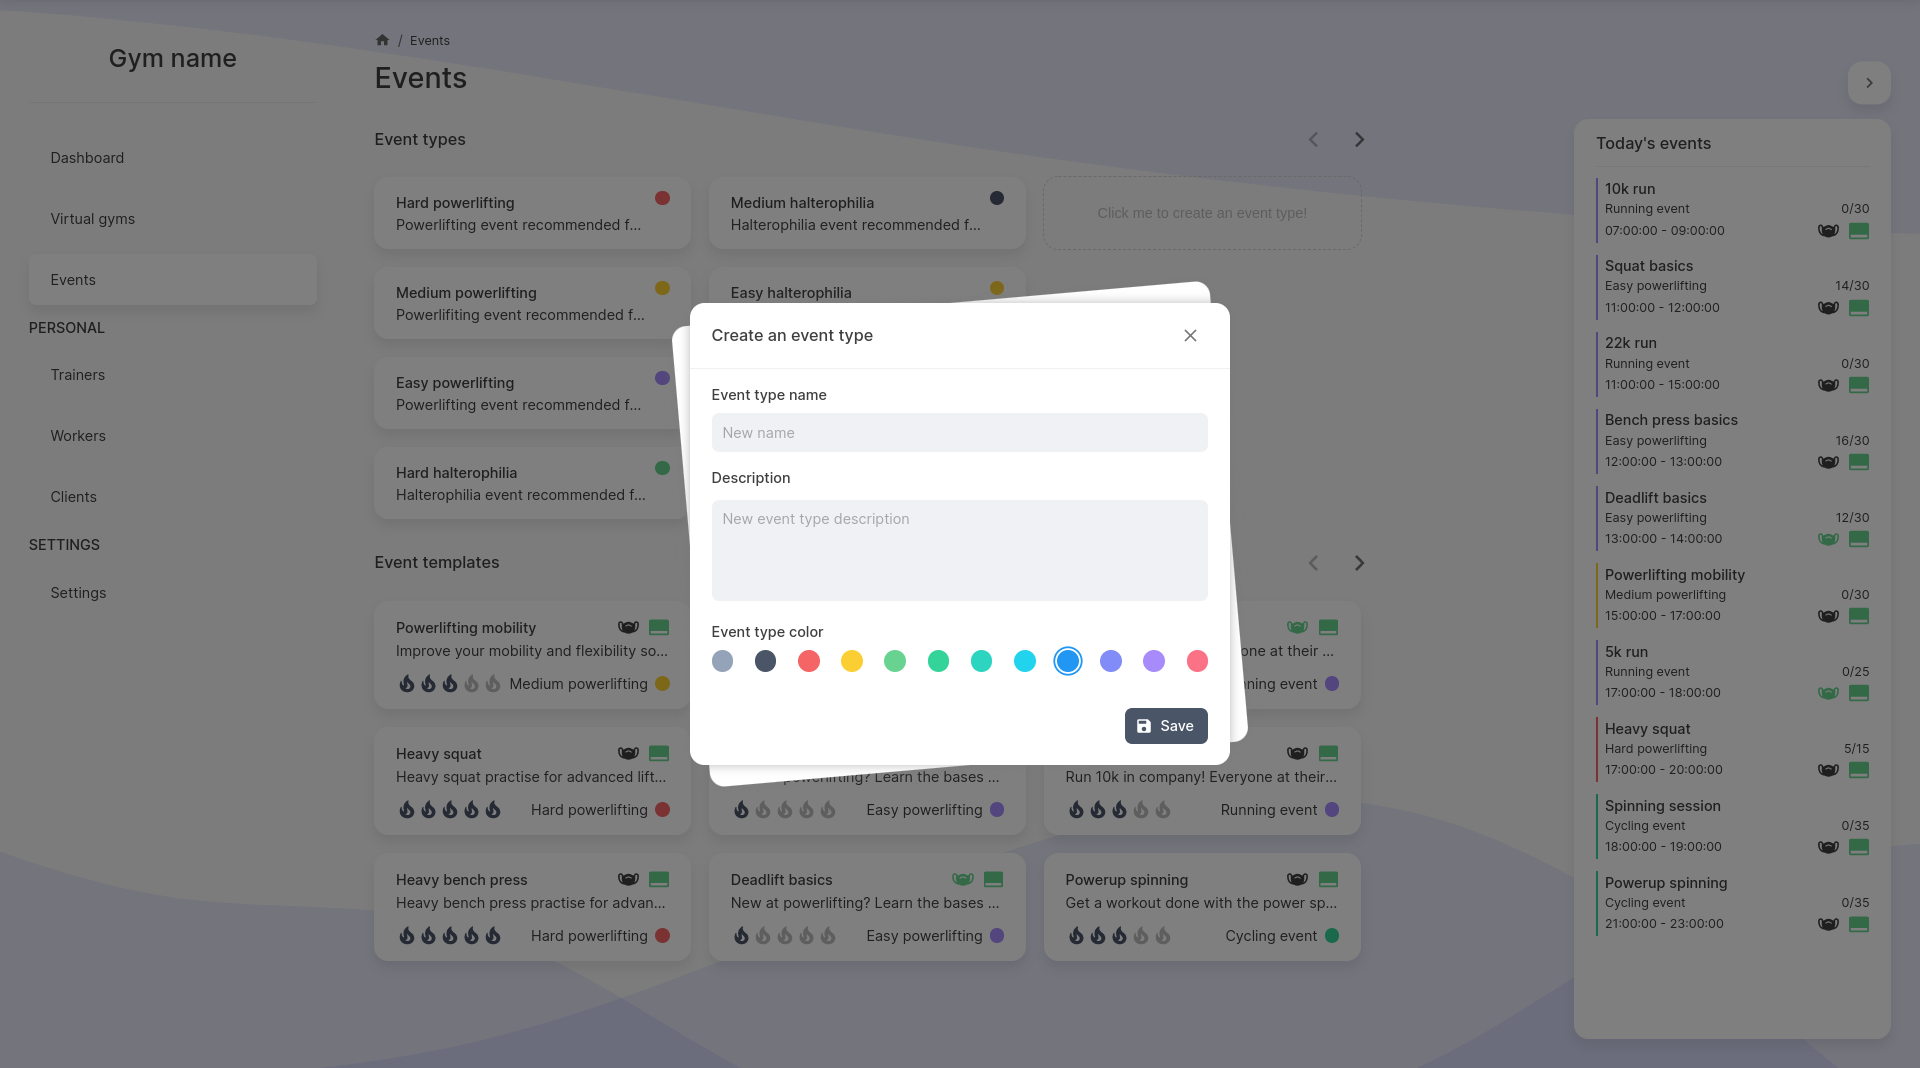
\includegraphics[width=\textwidth]{assets/core-screenshots/create-event-type.png}
	\caption{Creation of an event type}
\end{figure}
\begin{figure}[H]
	\centering
	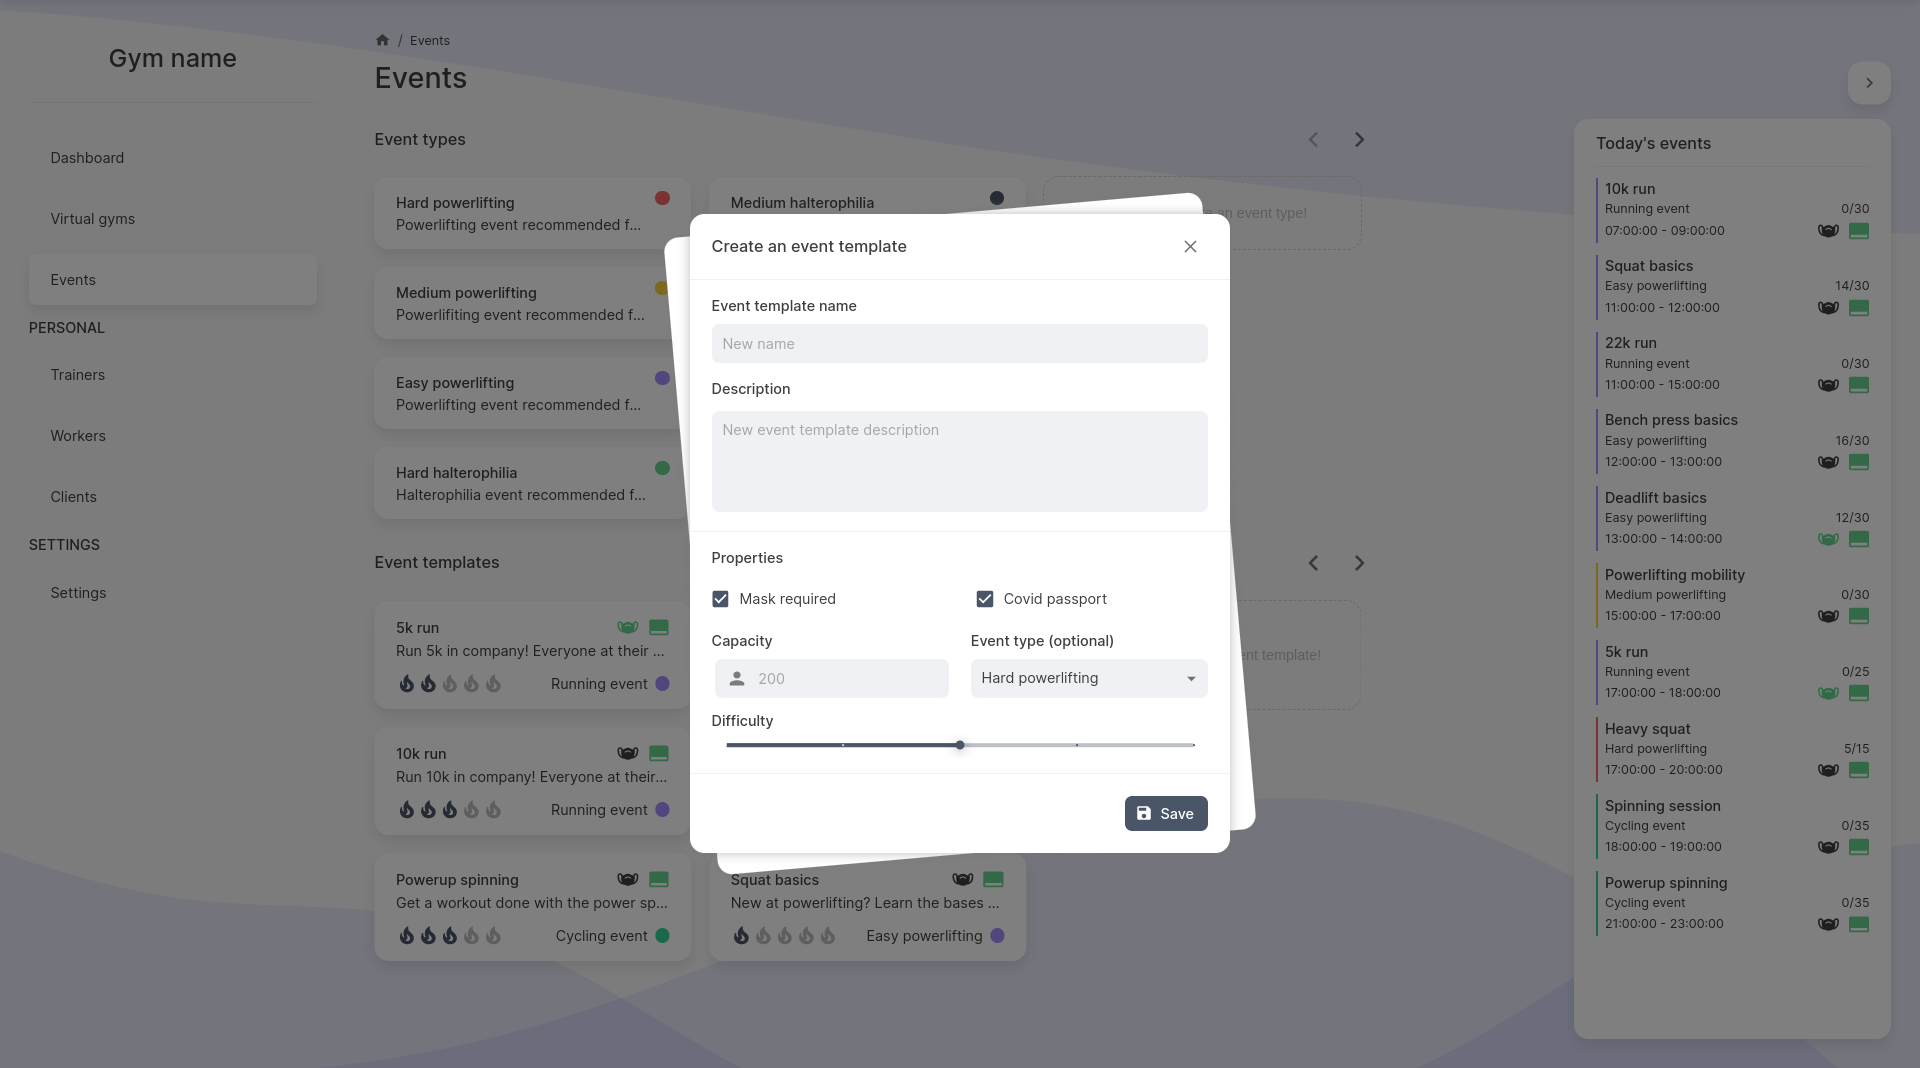
\includegraphics[width=\textwidth]{assets/core-screenshots/create-event-template.png}
	\caption{Creation of an event template}
\end{figure}
\subsubsection{Workers}
\begin{figure}[H]
	\centering
	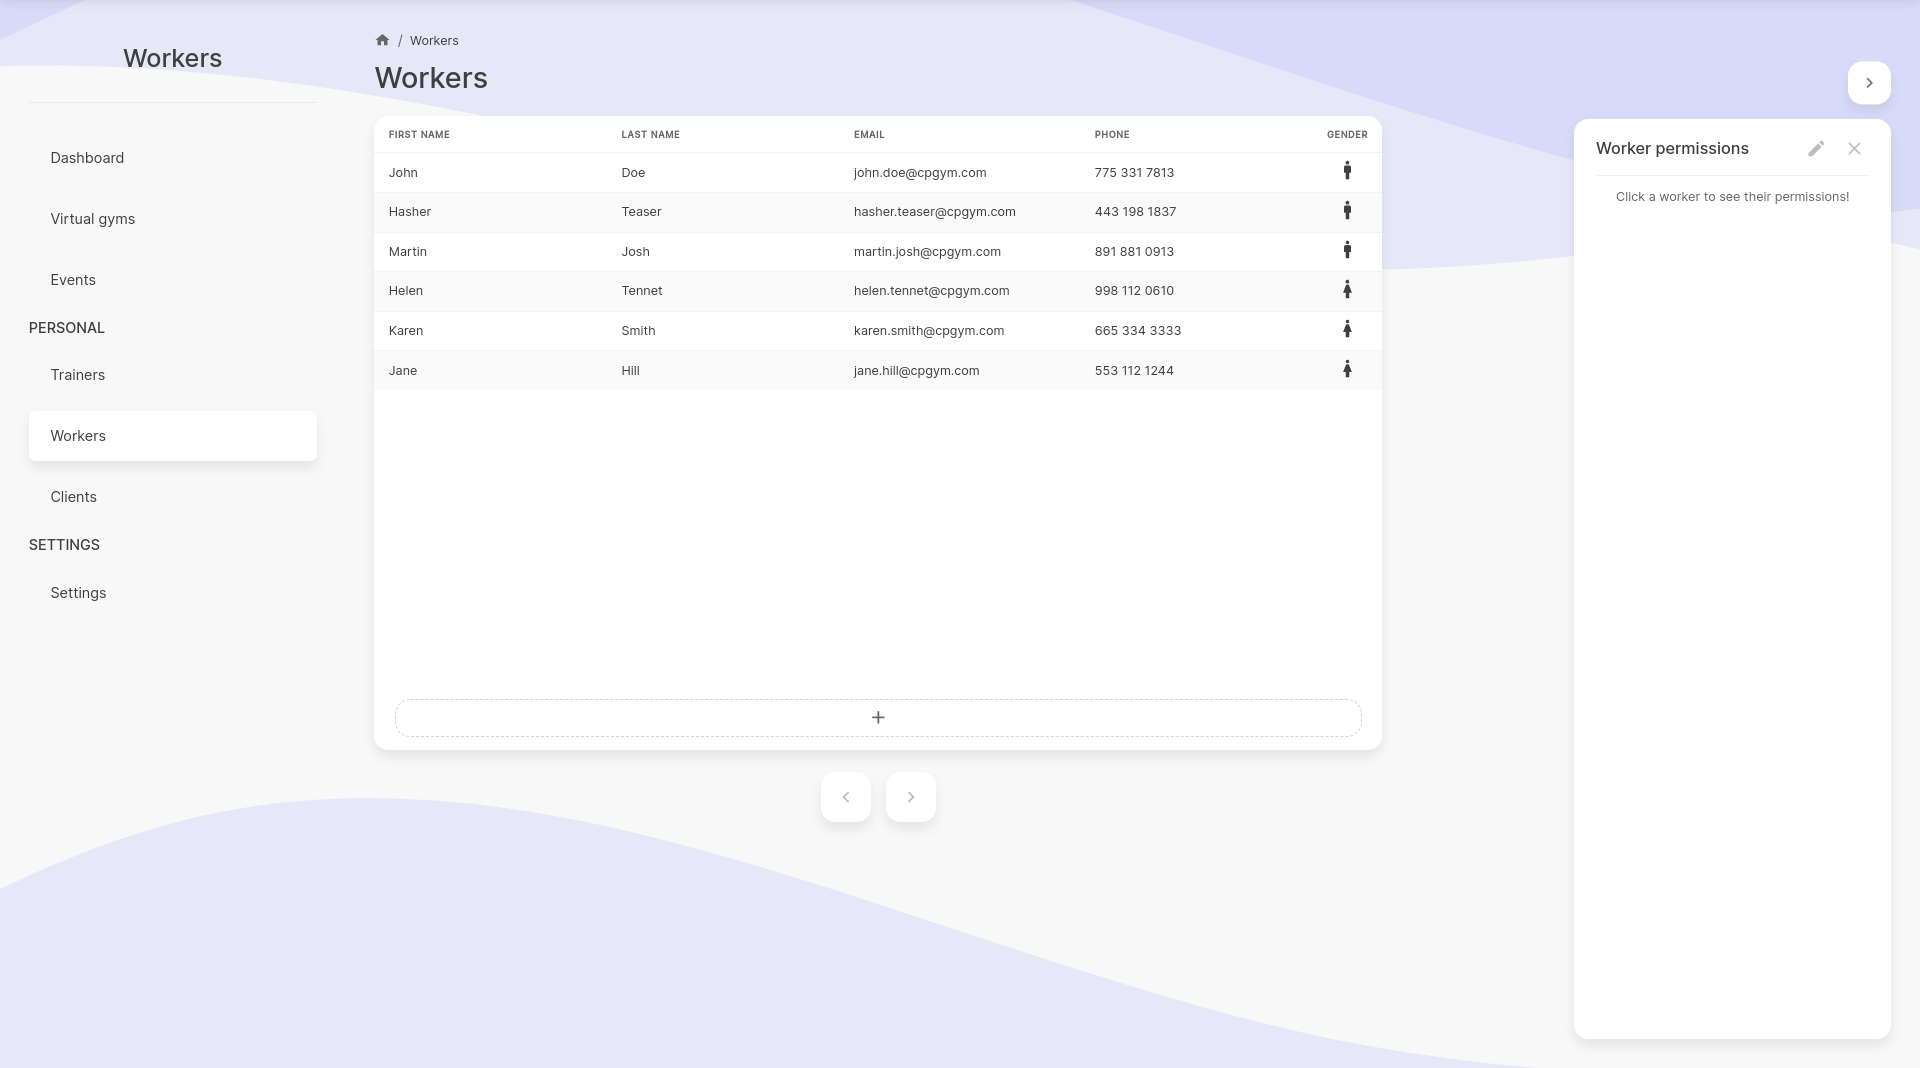
\includegraphics[width=\textwidth]{assets/core-screenshots/workers.png}
	\caption{Workers view without a worker selected}
\end{figure}
\begin{figure}[H]
	\centering
	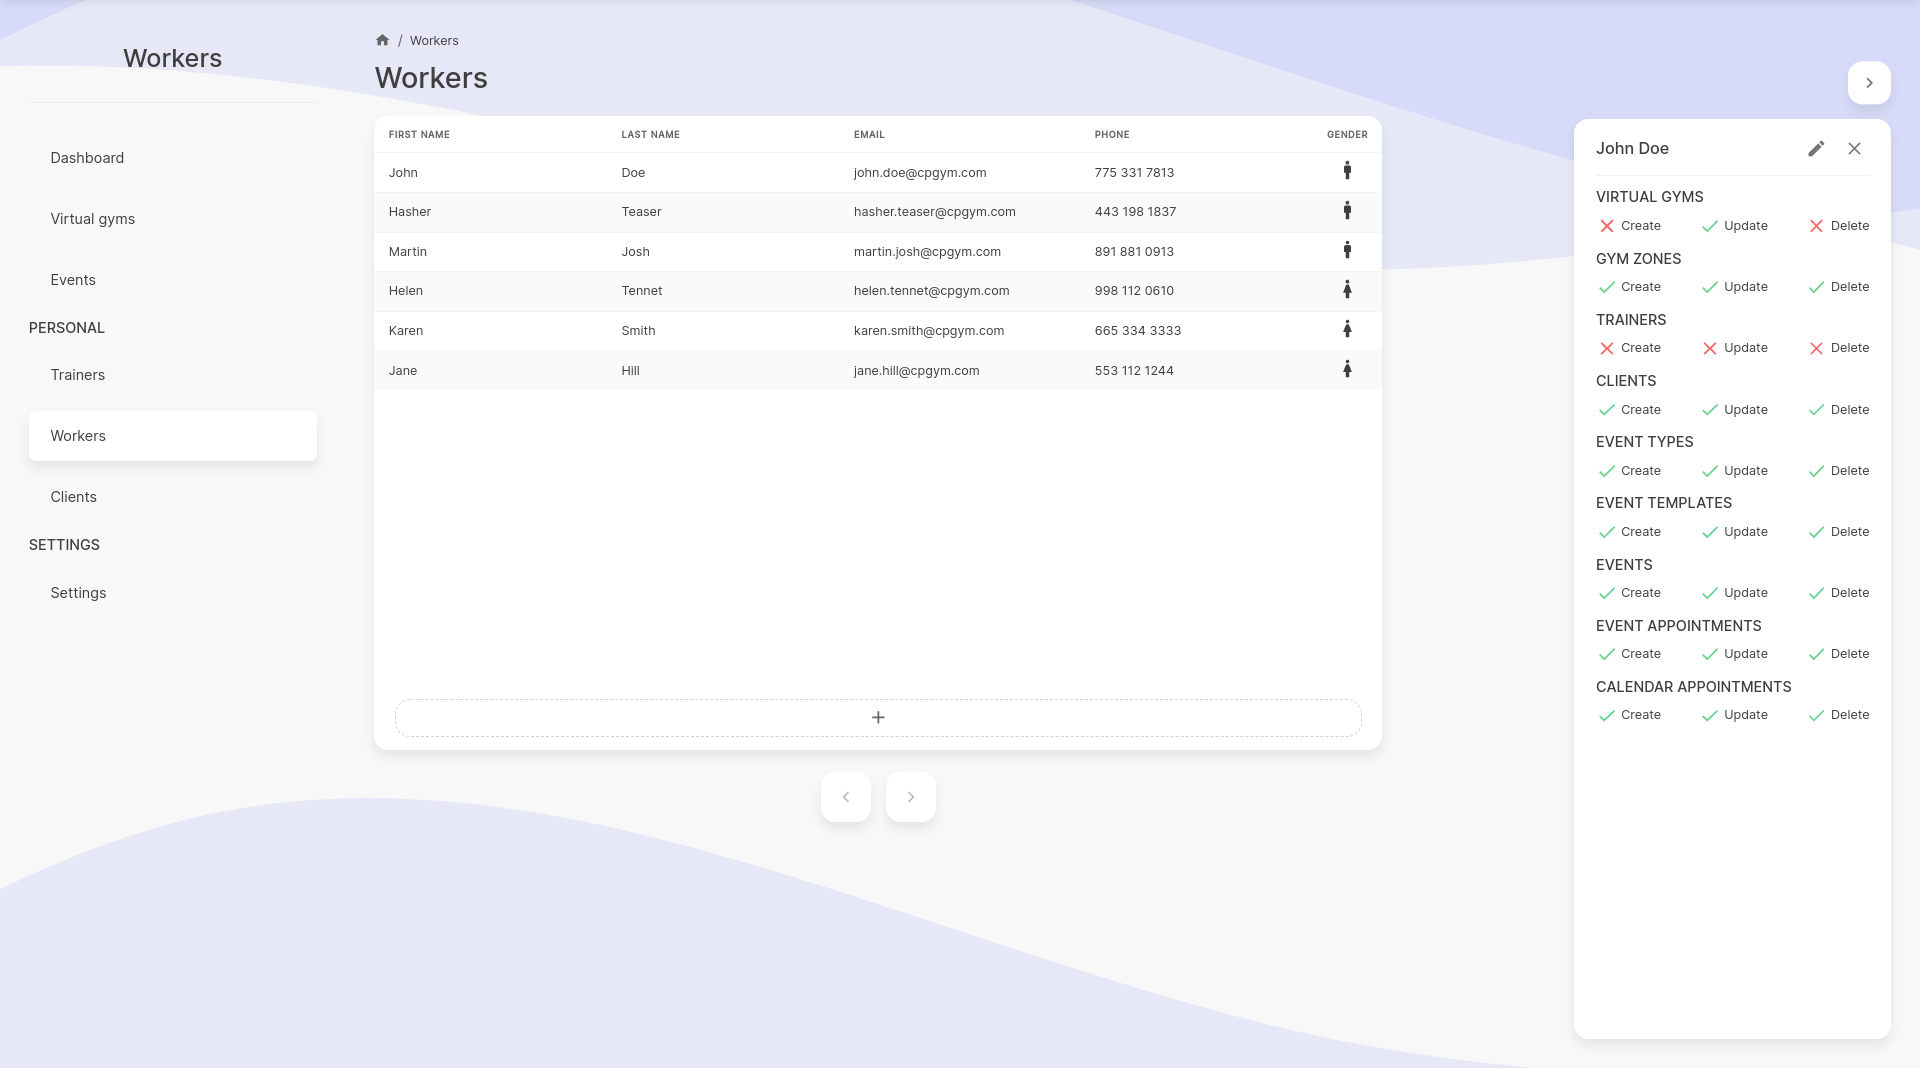
\includegraphics[width=\textwidth]{assets/core-screenshots/workers-selected.png}
	\caption{Workers view with a worker selected}
\end{figure}
\begin{figure}[H]
	\centering
	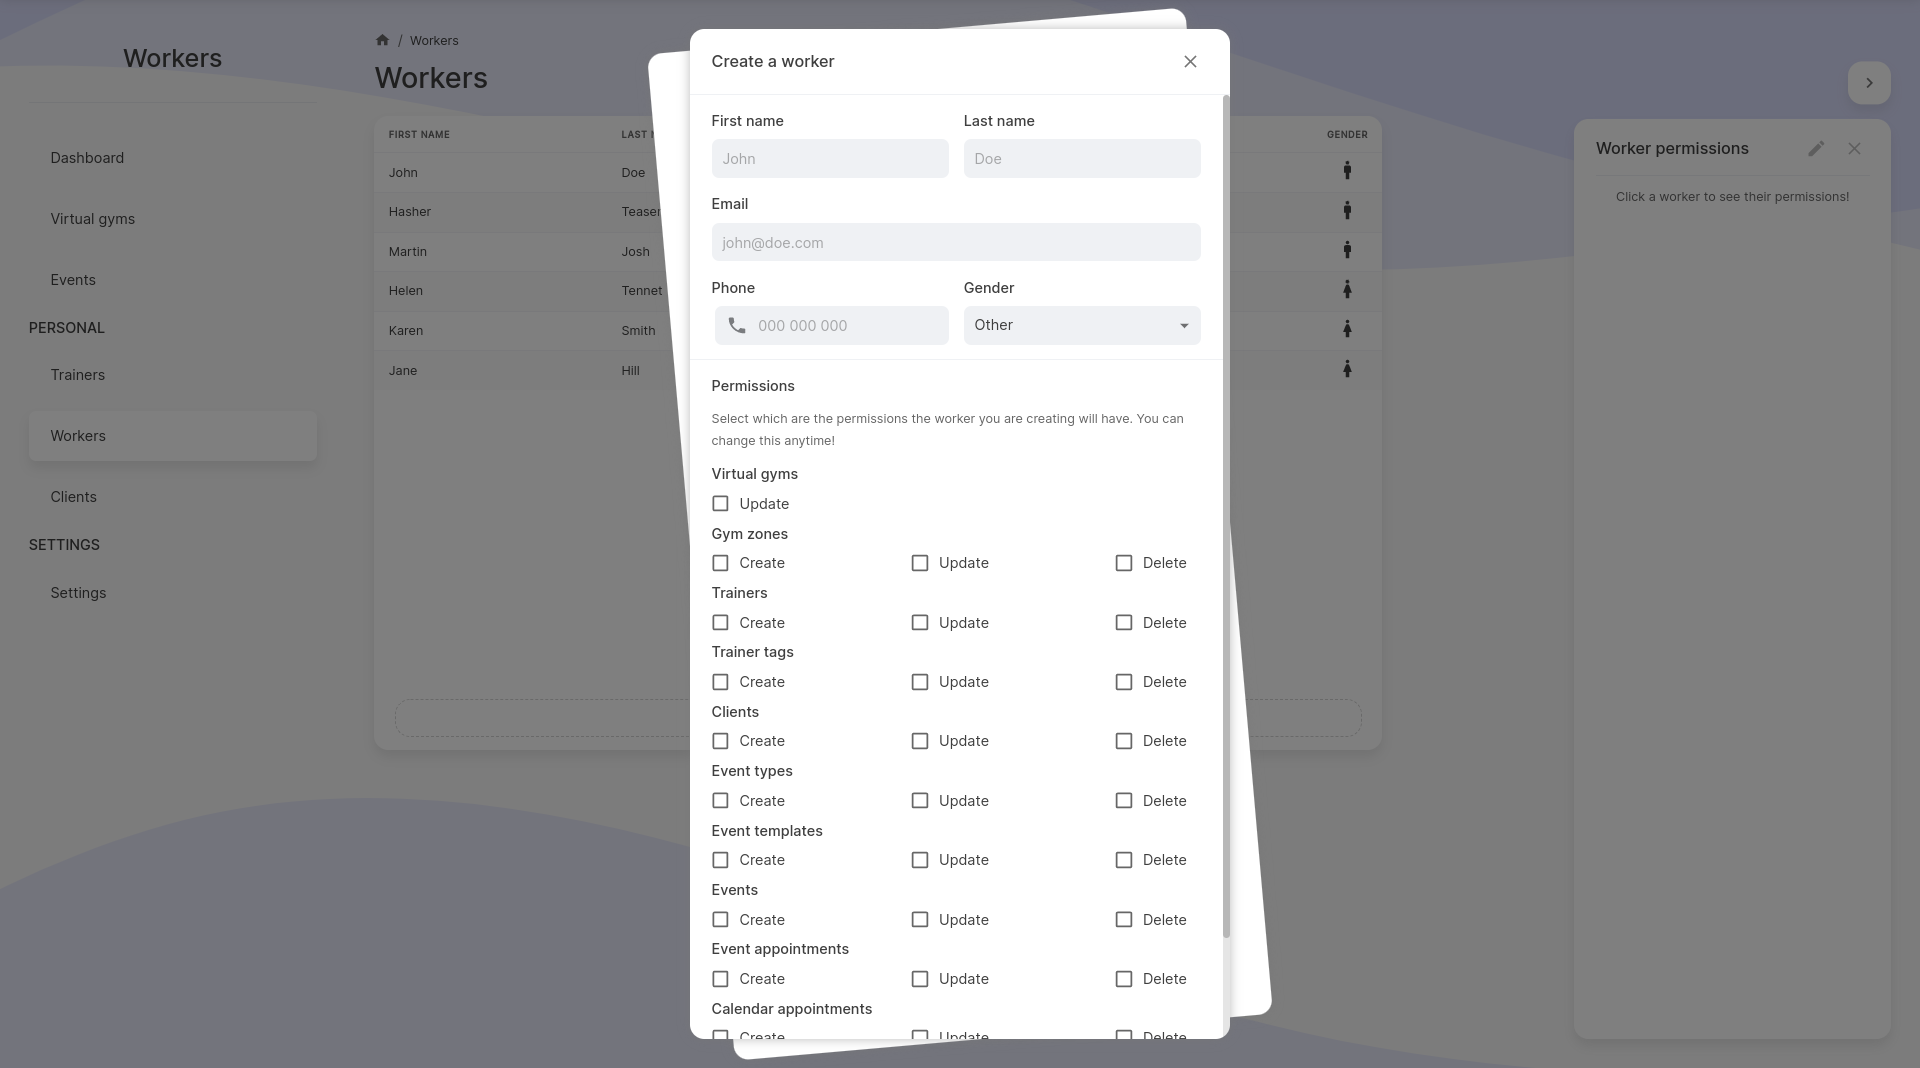
\includegraphics[width=\textwidth]{assets/core-screenshots/create-worker.png}
	\caption{Creation of a worker}
\end{figure}
\subsubsection{Trainers}
\begin{figure}[H]
	\centering
	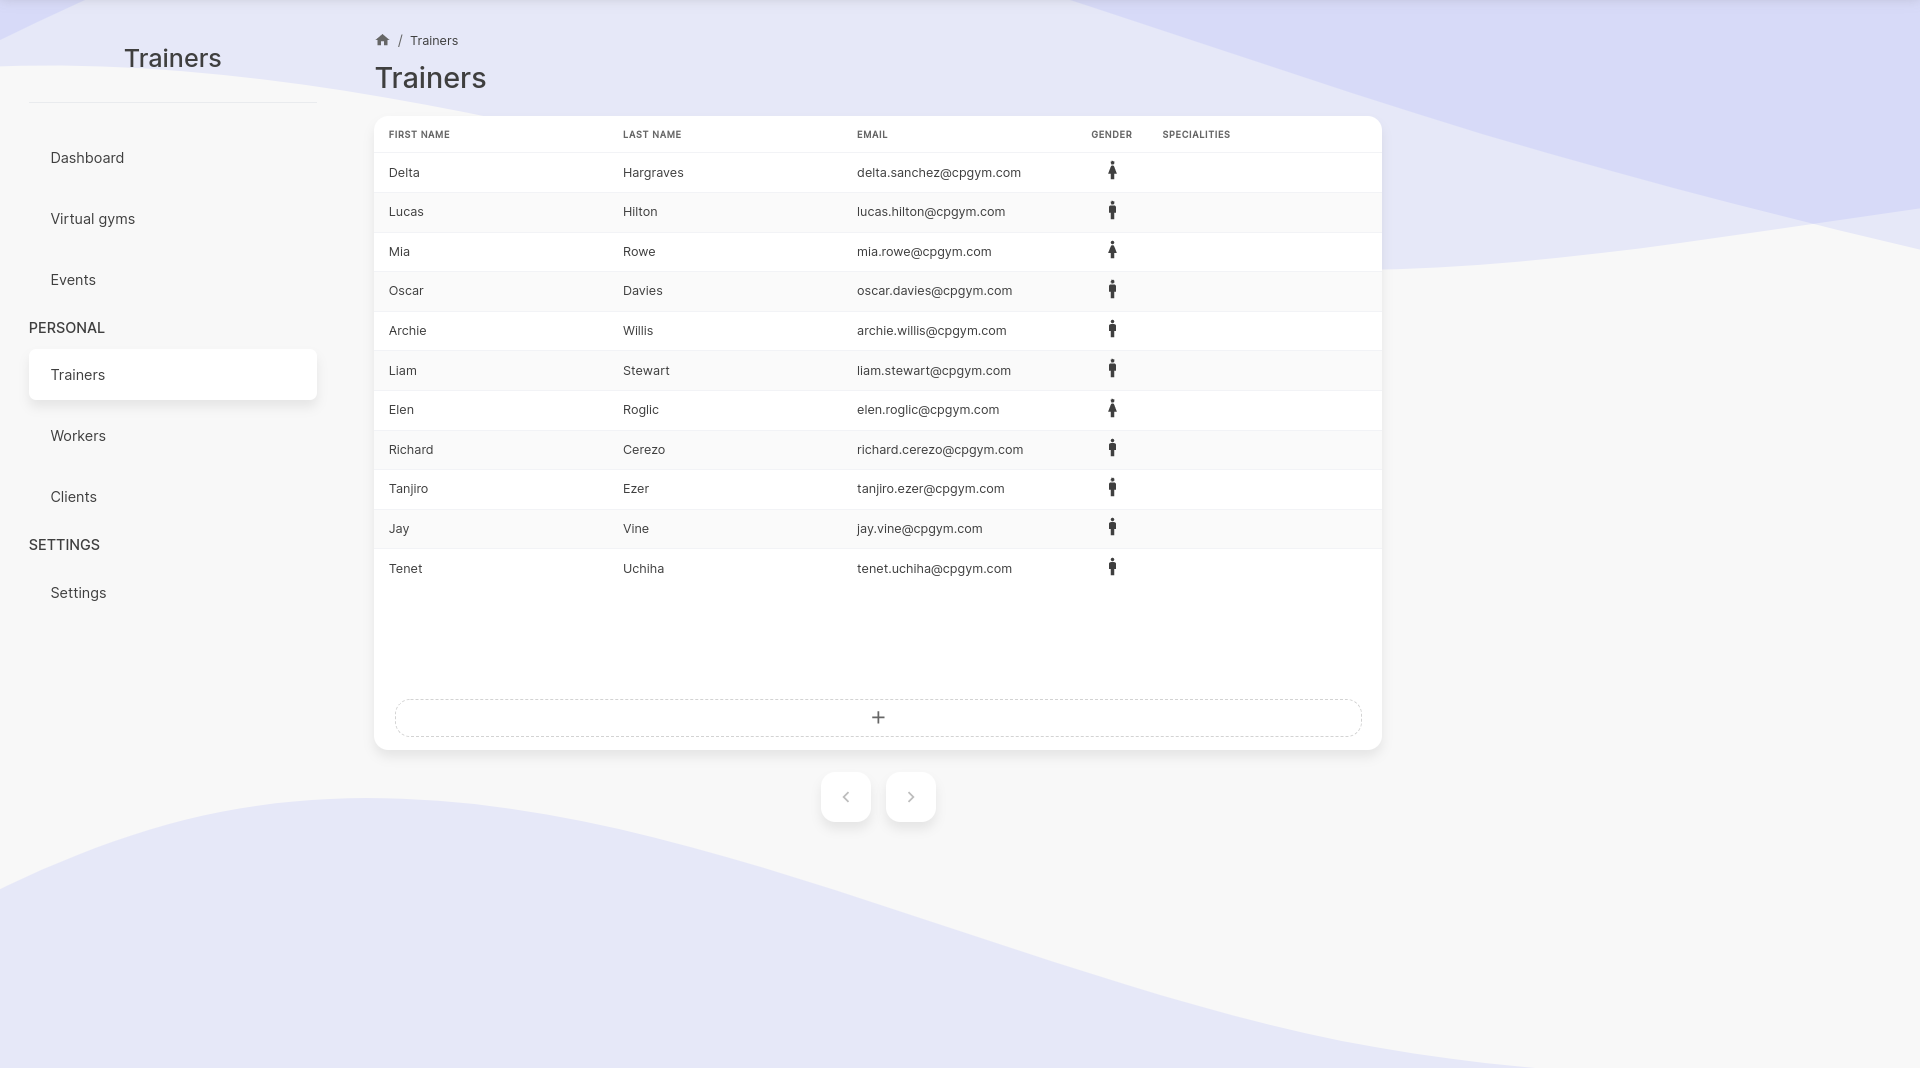
\includegraphics[width=\textwidth]{assets/core-screenshots/trainers.png}
	\caption{Trainers page}
\end{figure}
\begin{figure}[H]
	\centering
	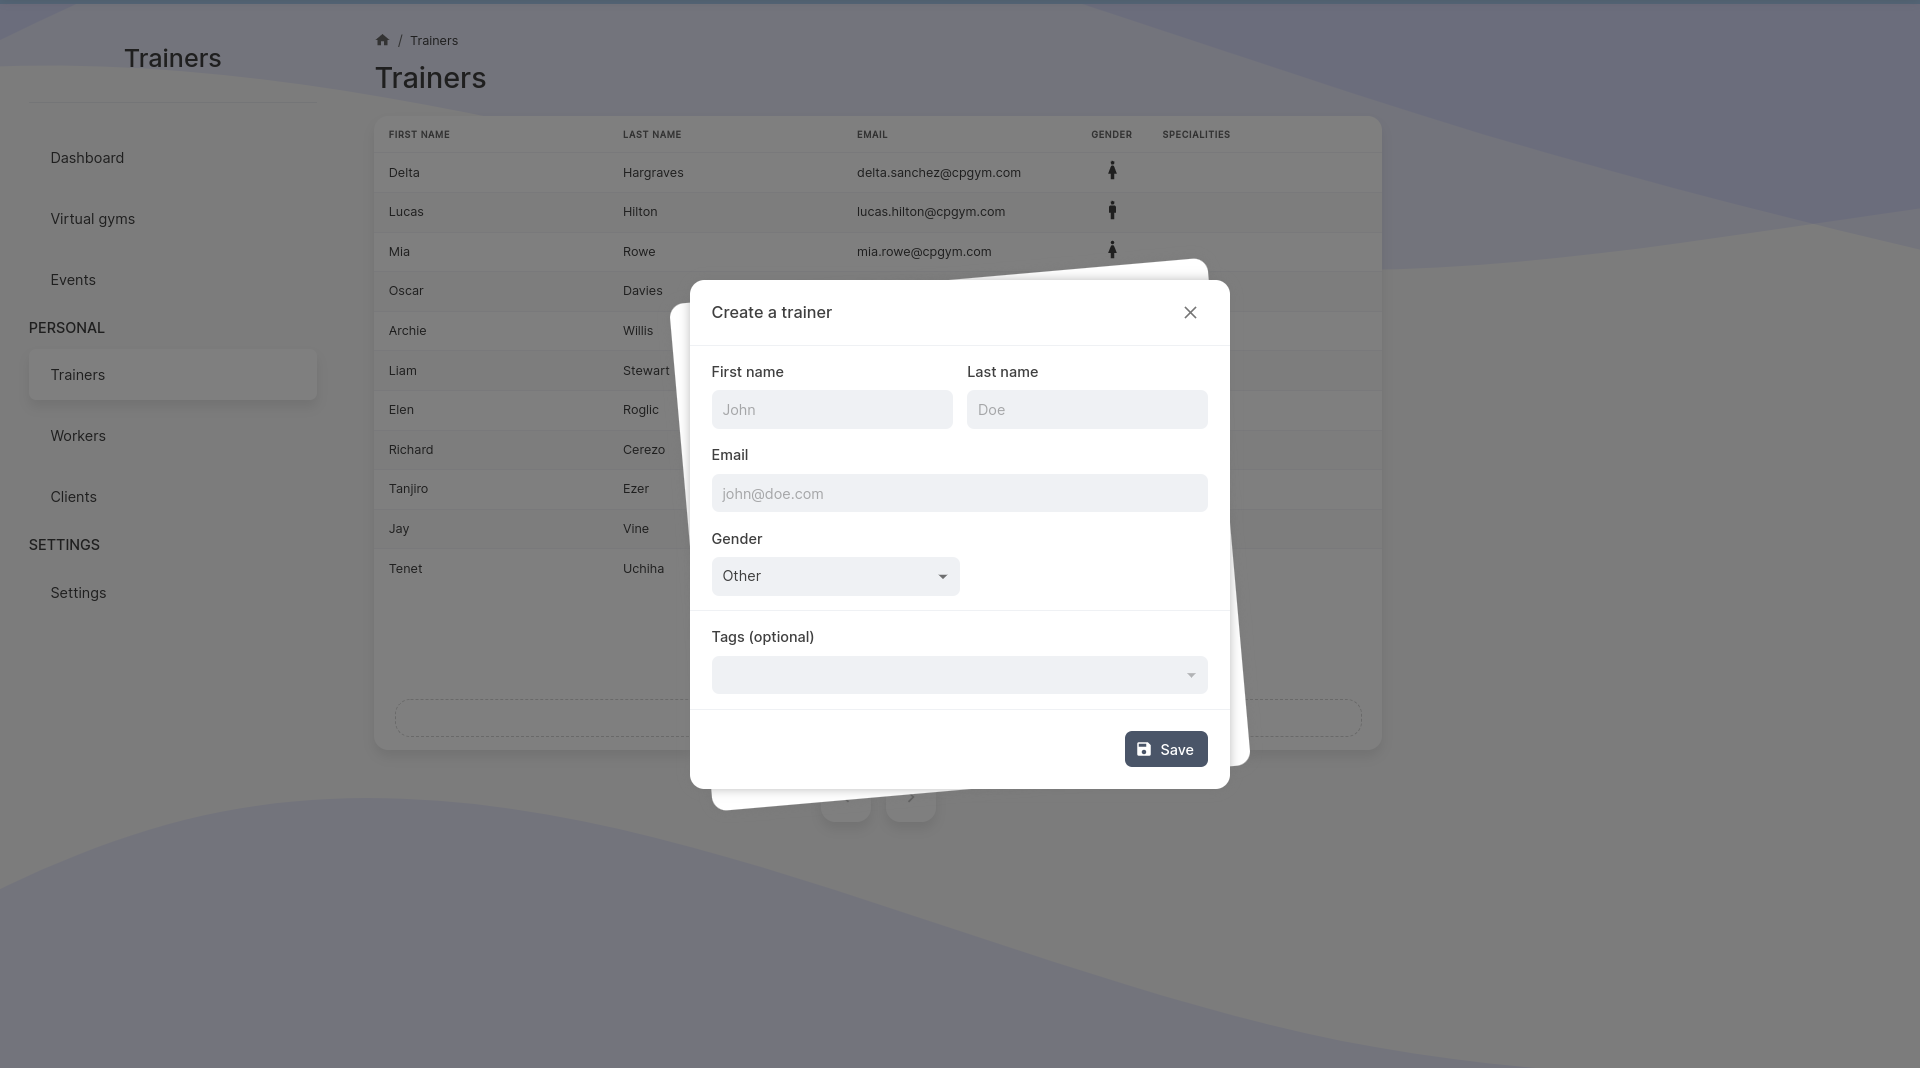
\includegraphics[width=\textwidth]{assets/core-screenshots/create-trainer.png}
	\caption{Creation of a trainer}
\end{figure}
\subsubsection{Clients}
\begin{figure}[H]
	\centering
	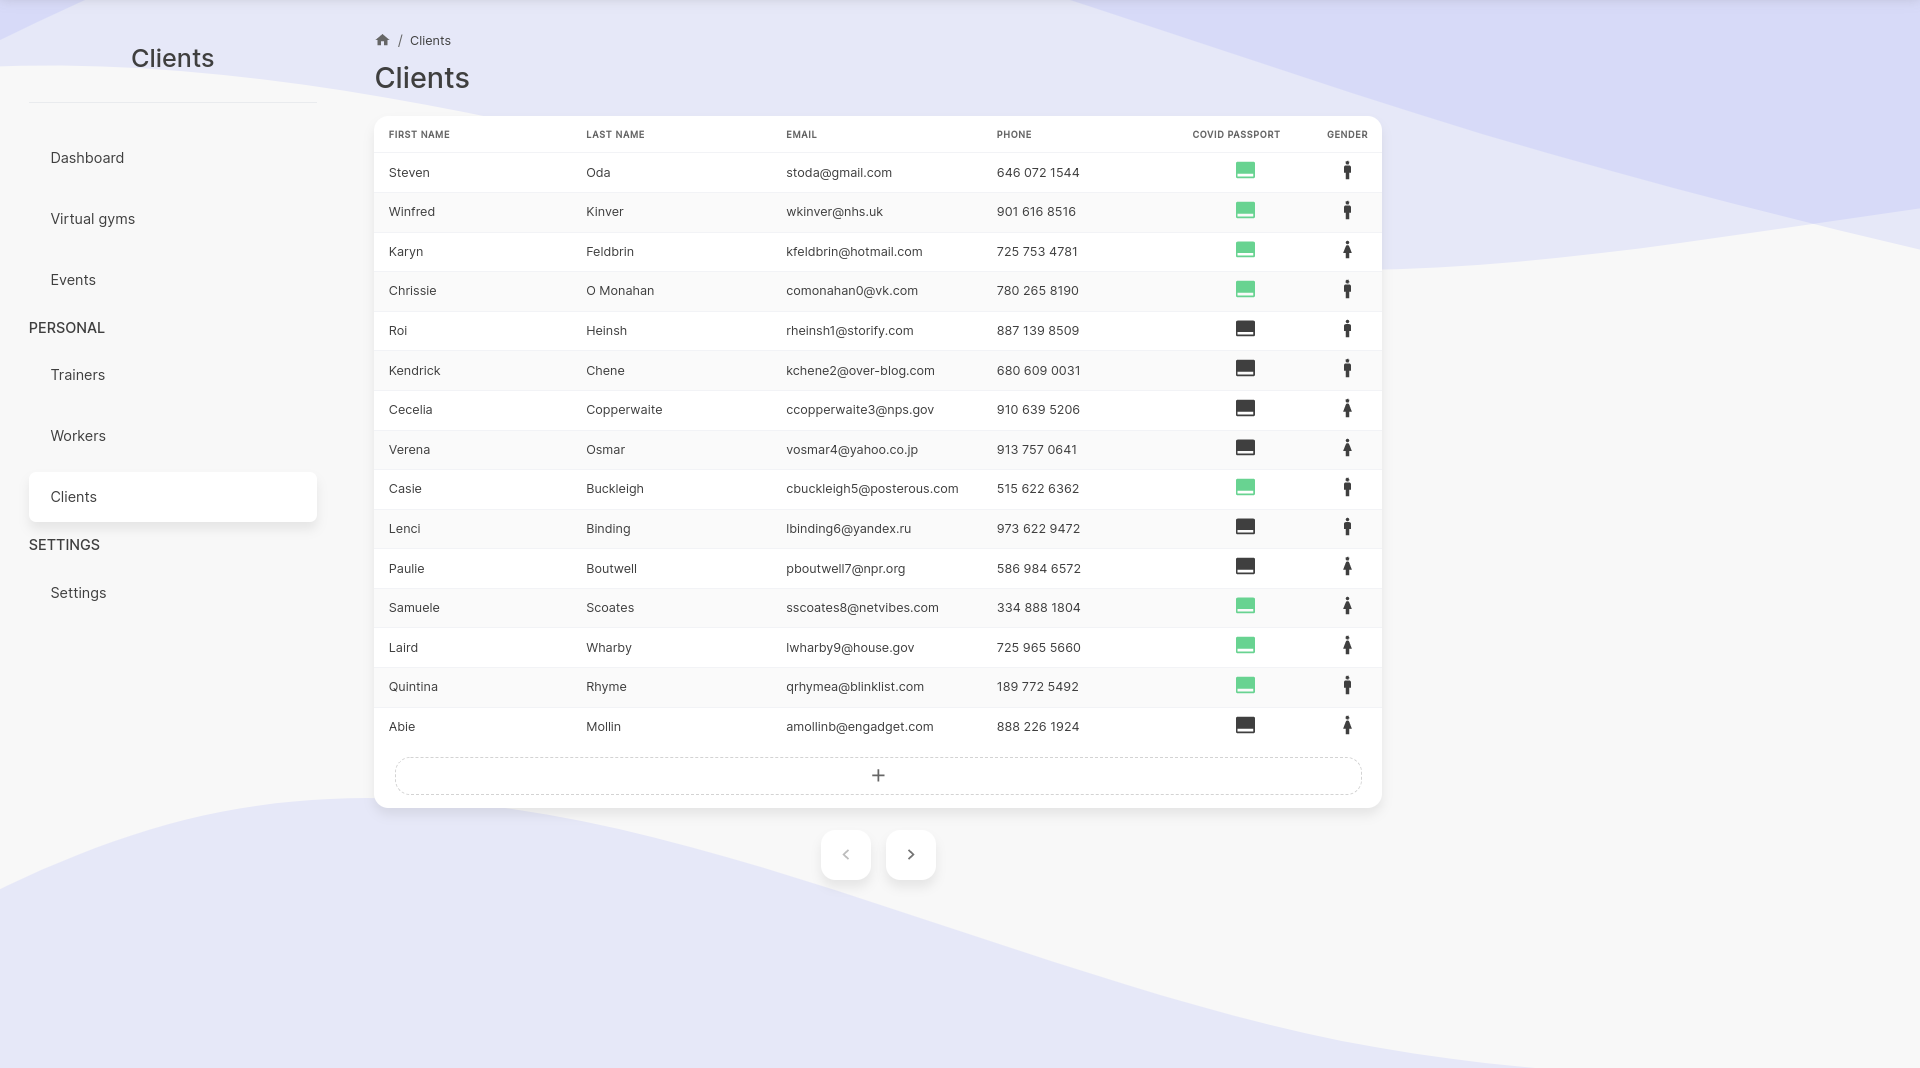
\includegraphics[width=\textwidth]{assets/core-screenshots/clients.png}
	\caption{Clients page}
\end{figure}
\begin{figure}[H]
	\centering
	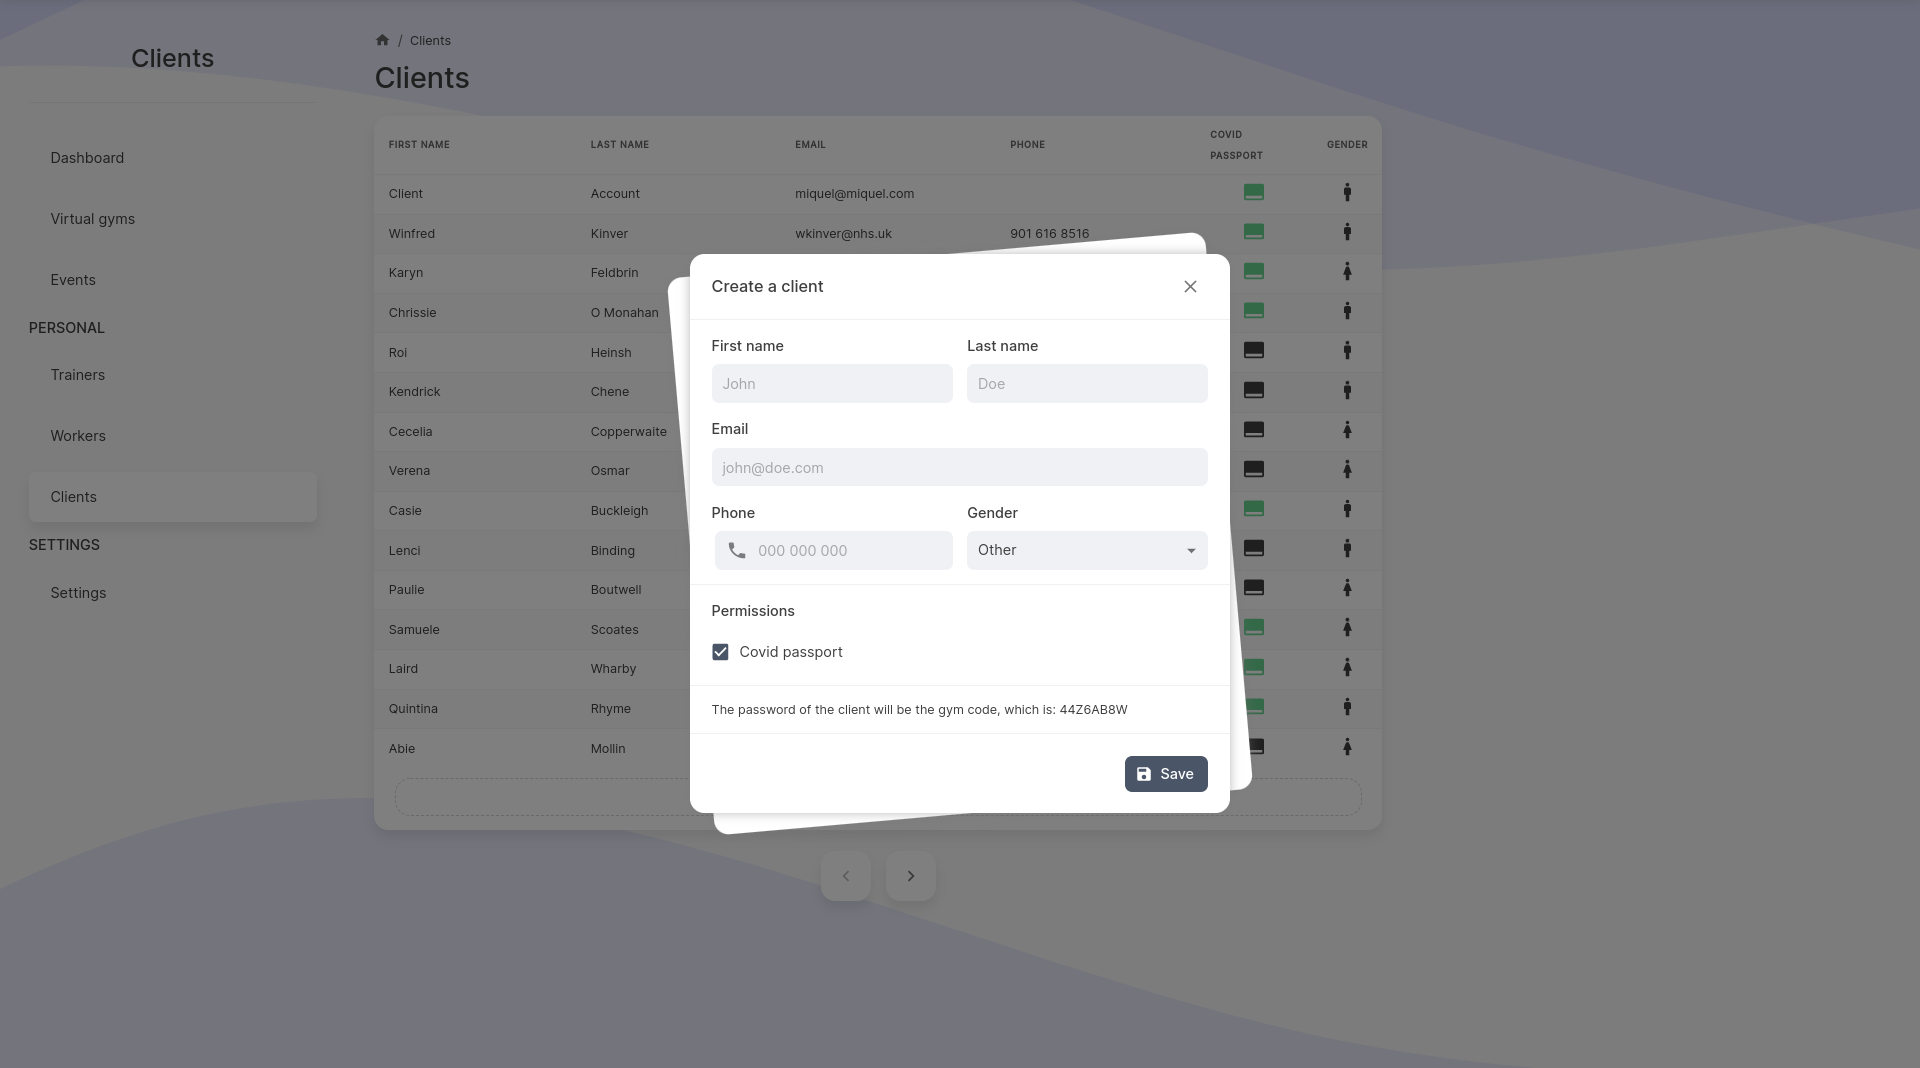
\includegraphics[width=\textwidth]{assets/core-screenshots/create-client.png}
	\caption{Creation of a client}
\end{figure}
\subsubsection{Settings}
The settings page for a worker would look the same, without having the gym properties available.
\begin{figure}[H]
	\centering
	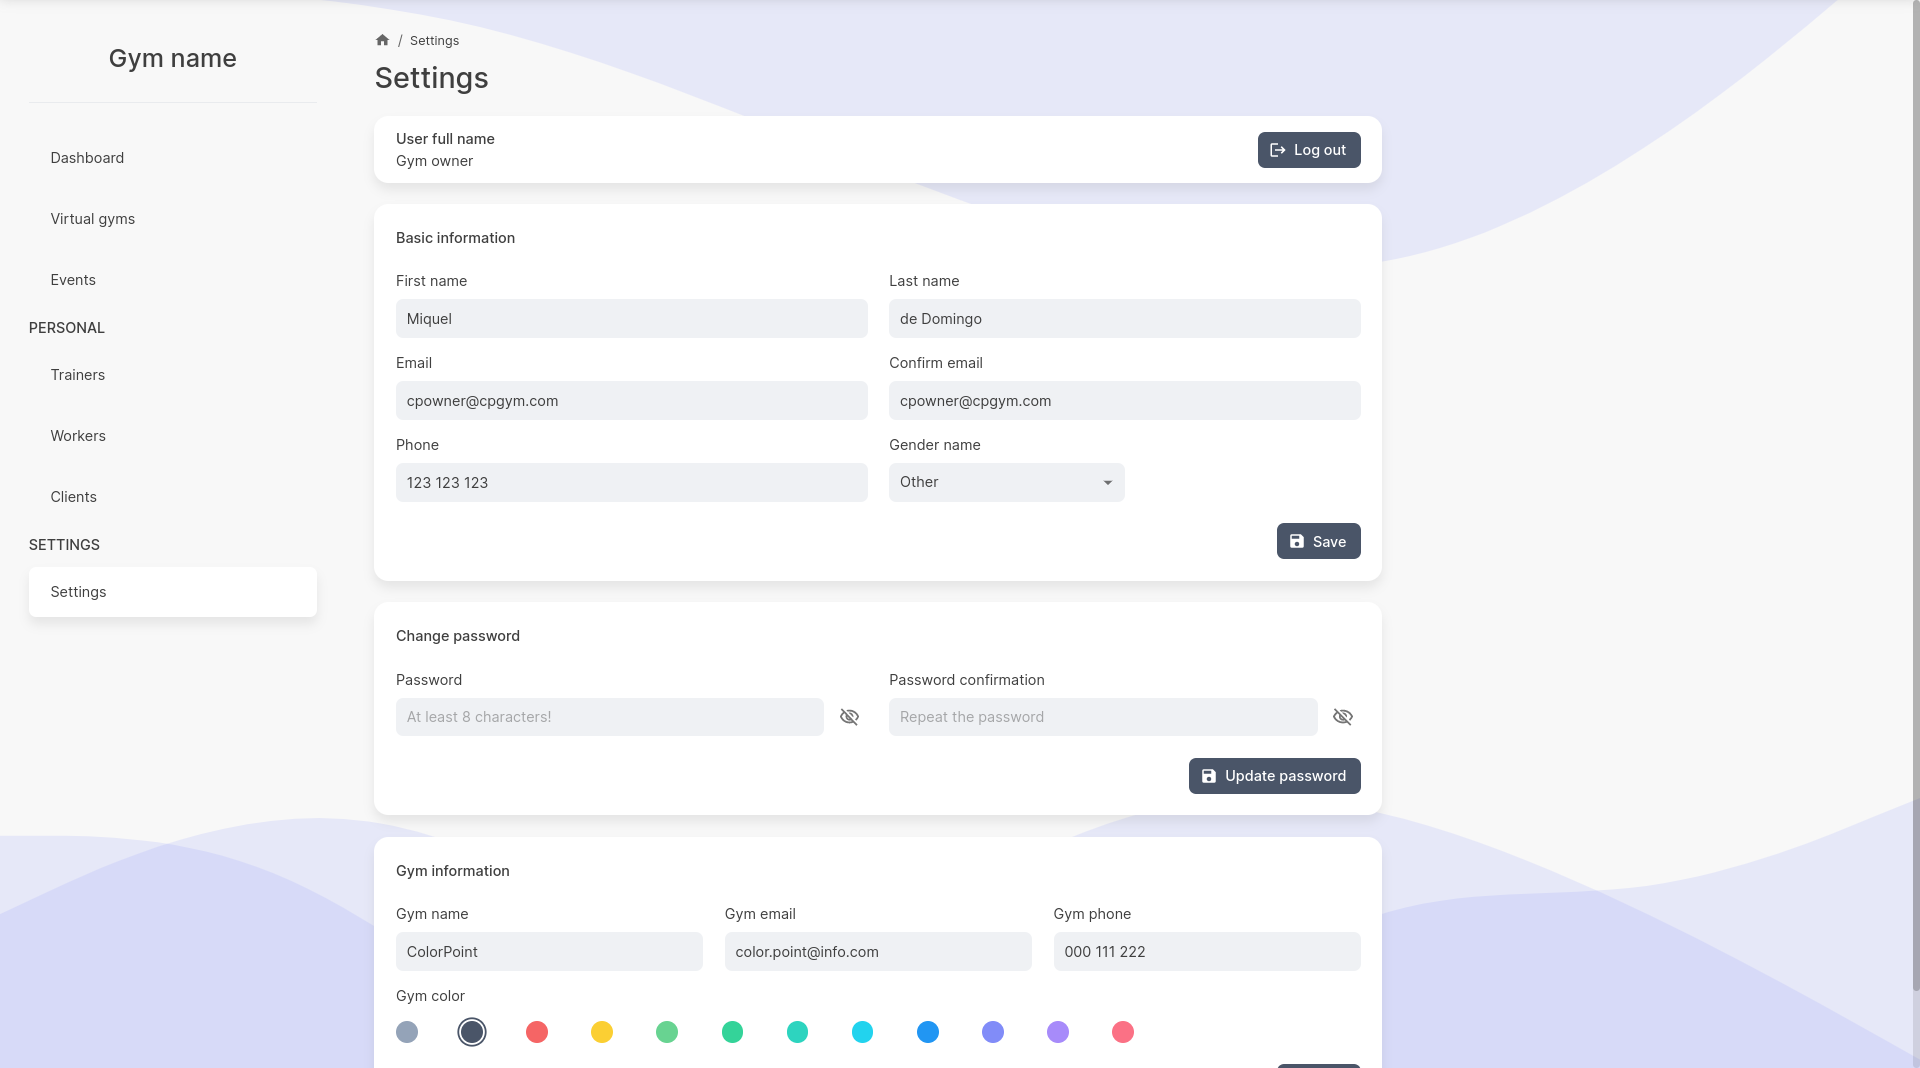
\includegraphics[width=\textwidth]{assets/core-screenshots/settings.png}
	\caption{Settings page}
\end{figure}
\subsection{Client application}
\subsubsection{Authentication}
\begin{figure}[H]
	\centering
	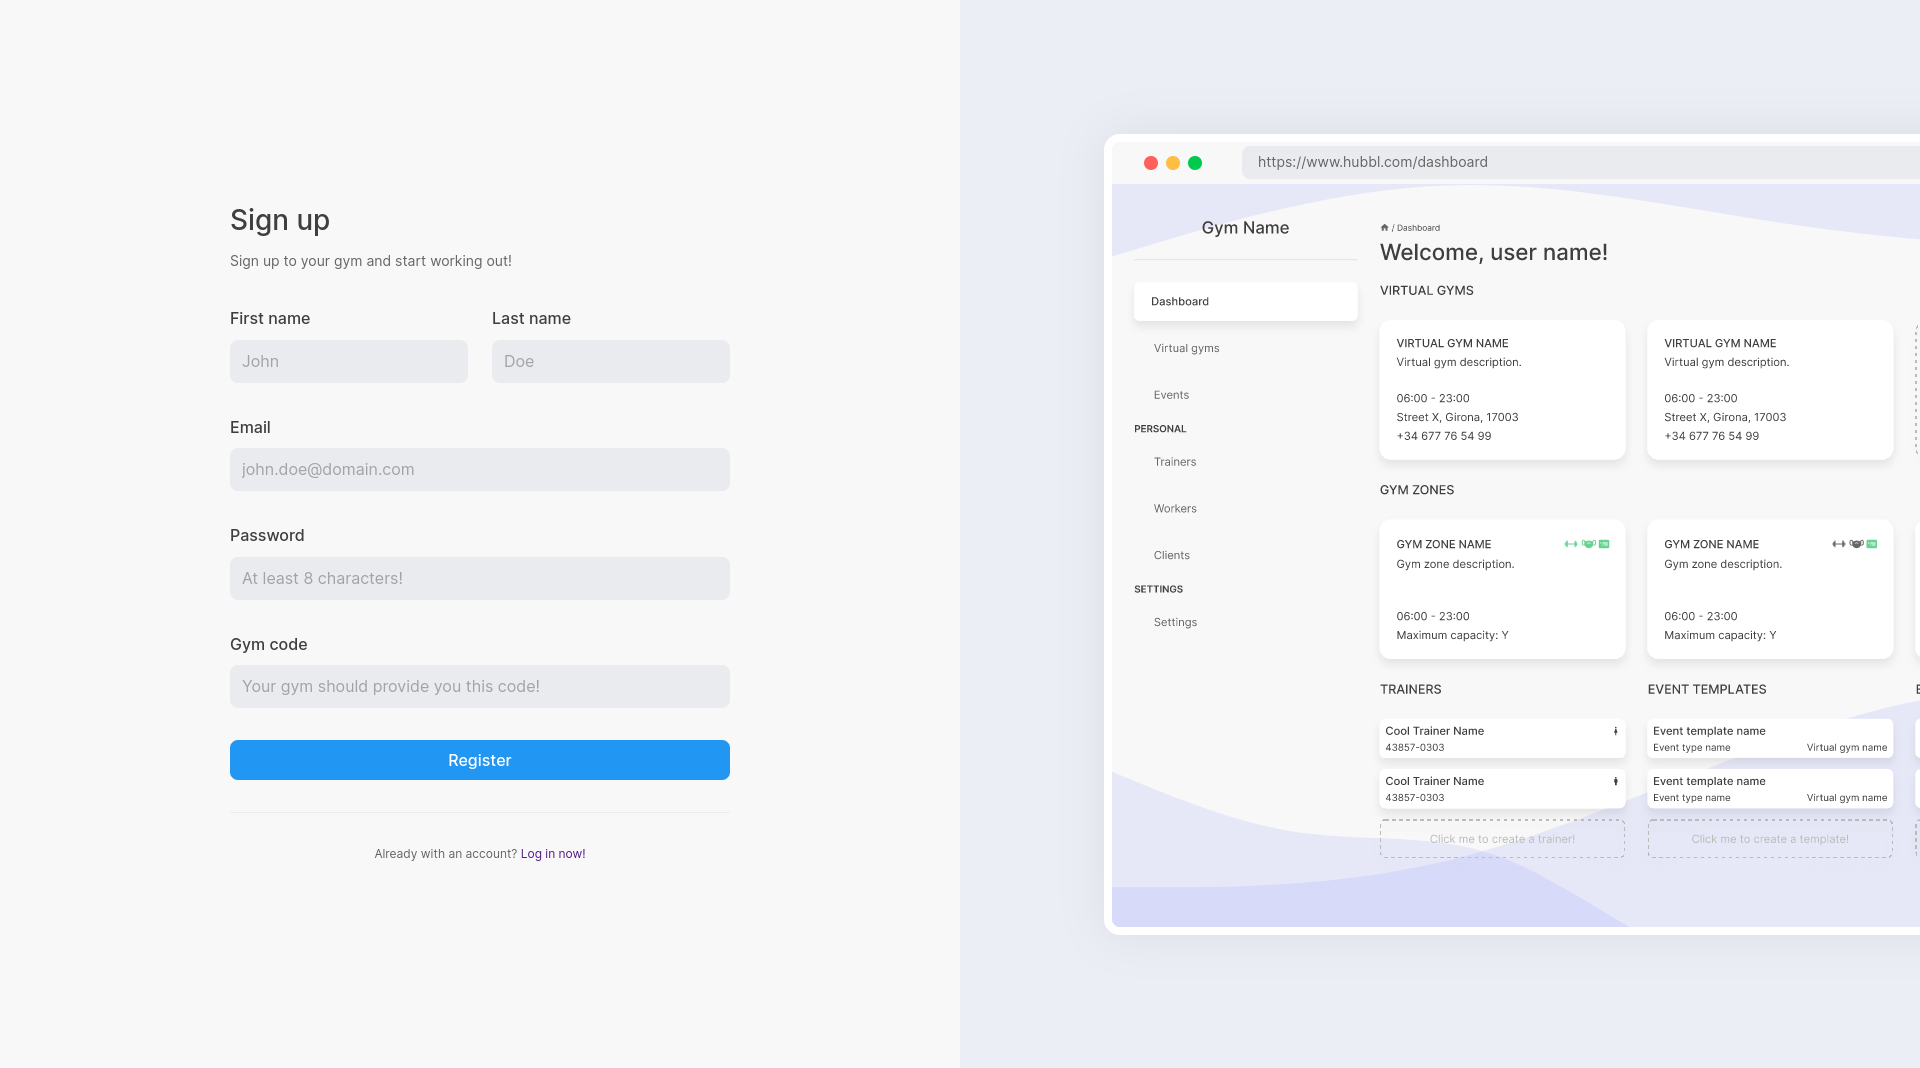
\includegraphics[width=\textwidth]{assets/client-screenshots/sign-up.png}
	\caption{Sign up page}
\end{figure}
\begin{figure}[H]
	\centering
	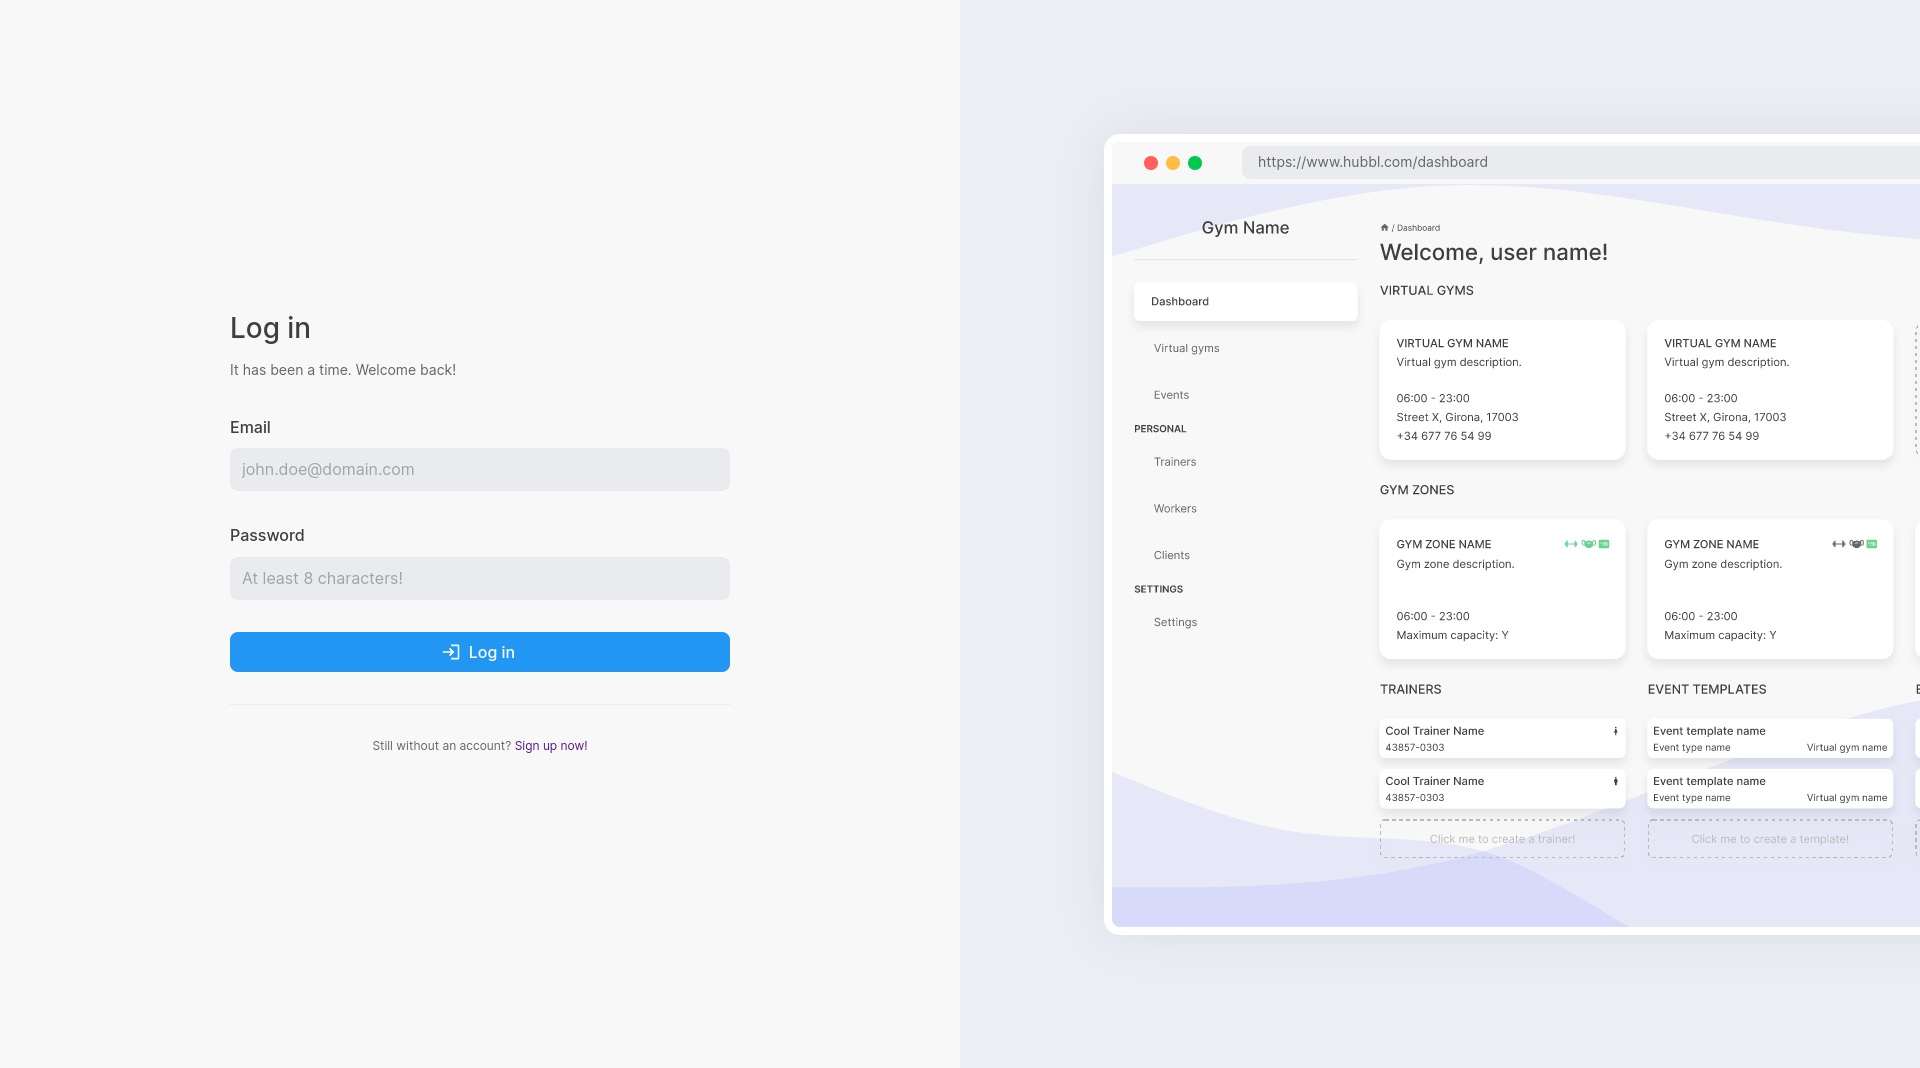
\includegraphics[width=\textwidth]{assets/client-screenshots/log-in.png}
	\caption{Log in page}
\end{figure}
\subsubsection{Dashboard page}
In comparison to the core application, the dasboard page contains fewer actions, and it is more simple.
\begin{figure}[H]
	\centering
	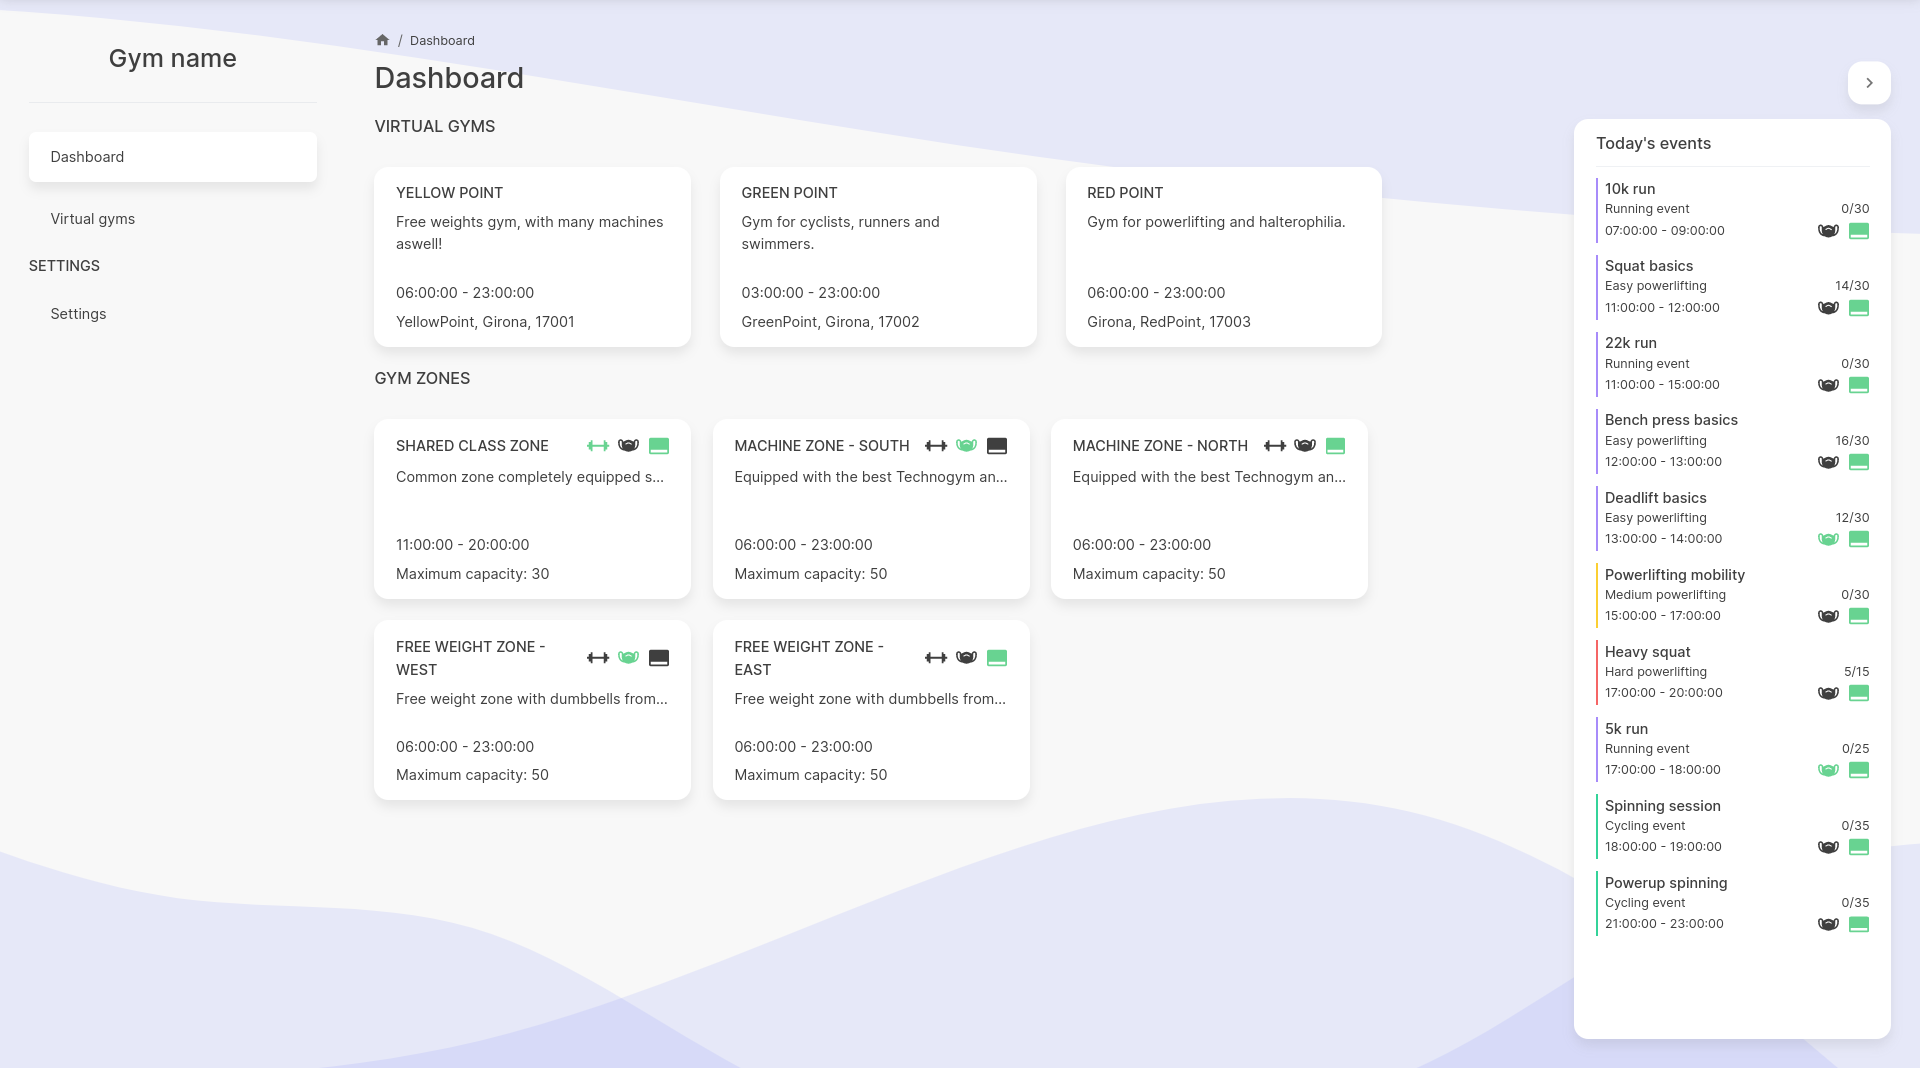
\includegraphics[width=\textwidth]{assets/client-screenshots/dashboard.png}
	\caption{Dashboard page}
\end{figure}
\subsubsection{Virtual gyms}
\begin{figure}[H]
	\centering
	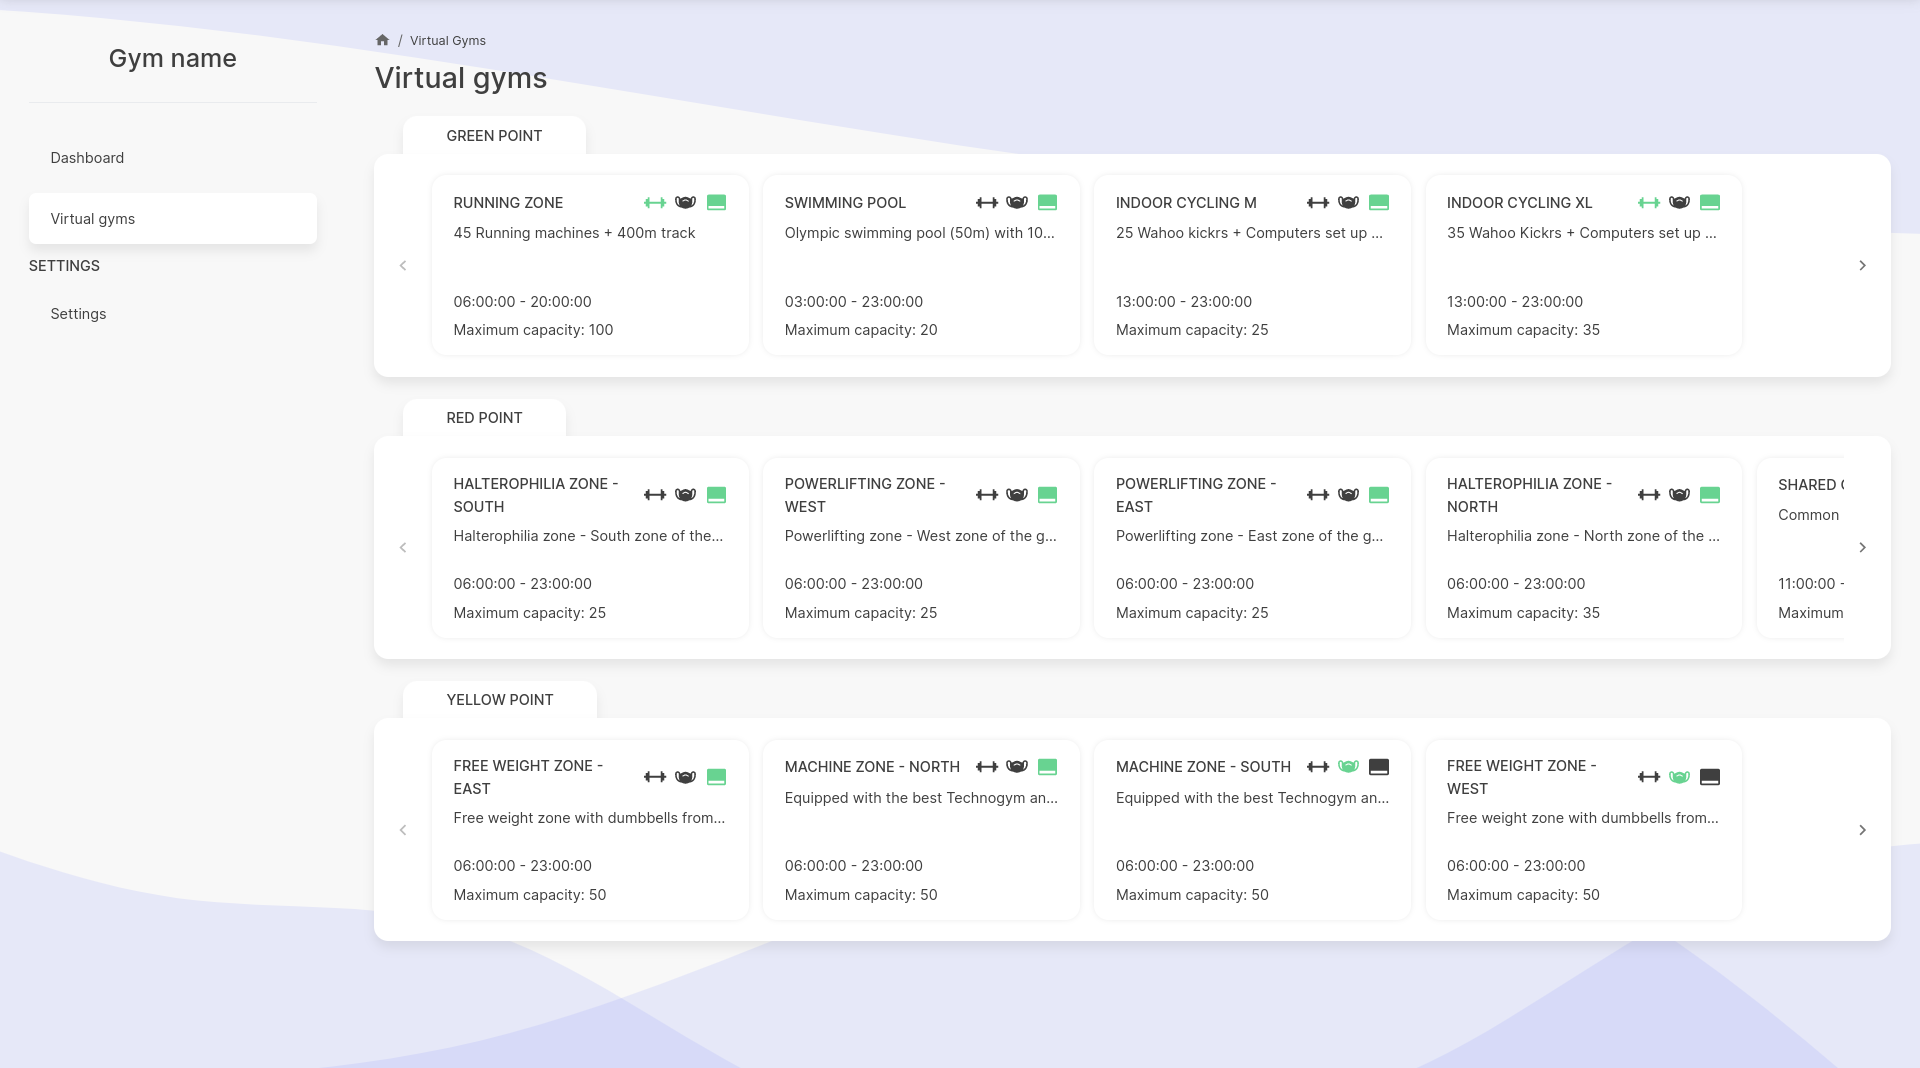
\includegraphics[width=\textwidth]{assets/client-screenshots/virtual-gyms.png}
	\caption{Virtual gyms page}
\end{figure}
Whenever a virtual gym has been clicked (by clicking at its name), the user is redirected to the above page, which displays all the gym zones of the chosen virtual gym.
\begin{figure}[H]
	\centering
	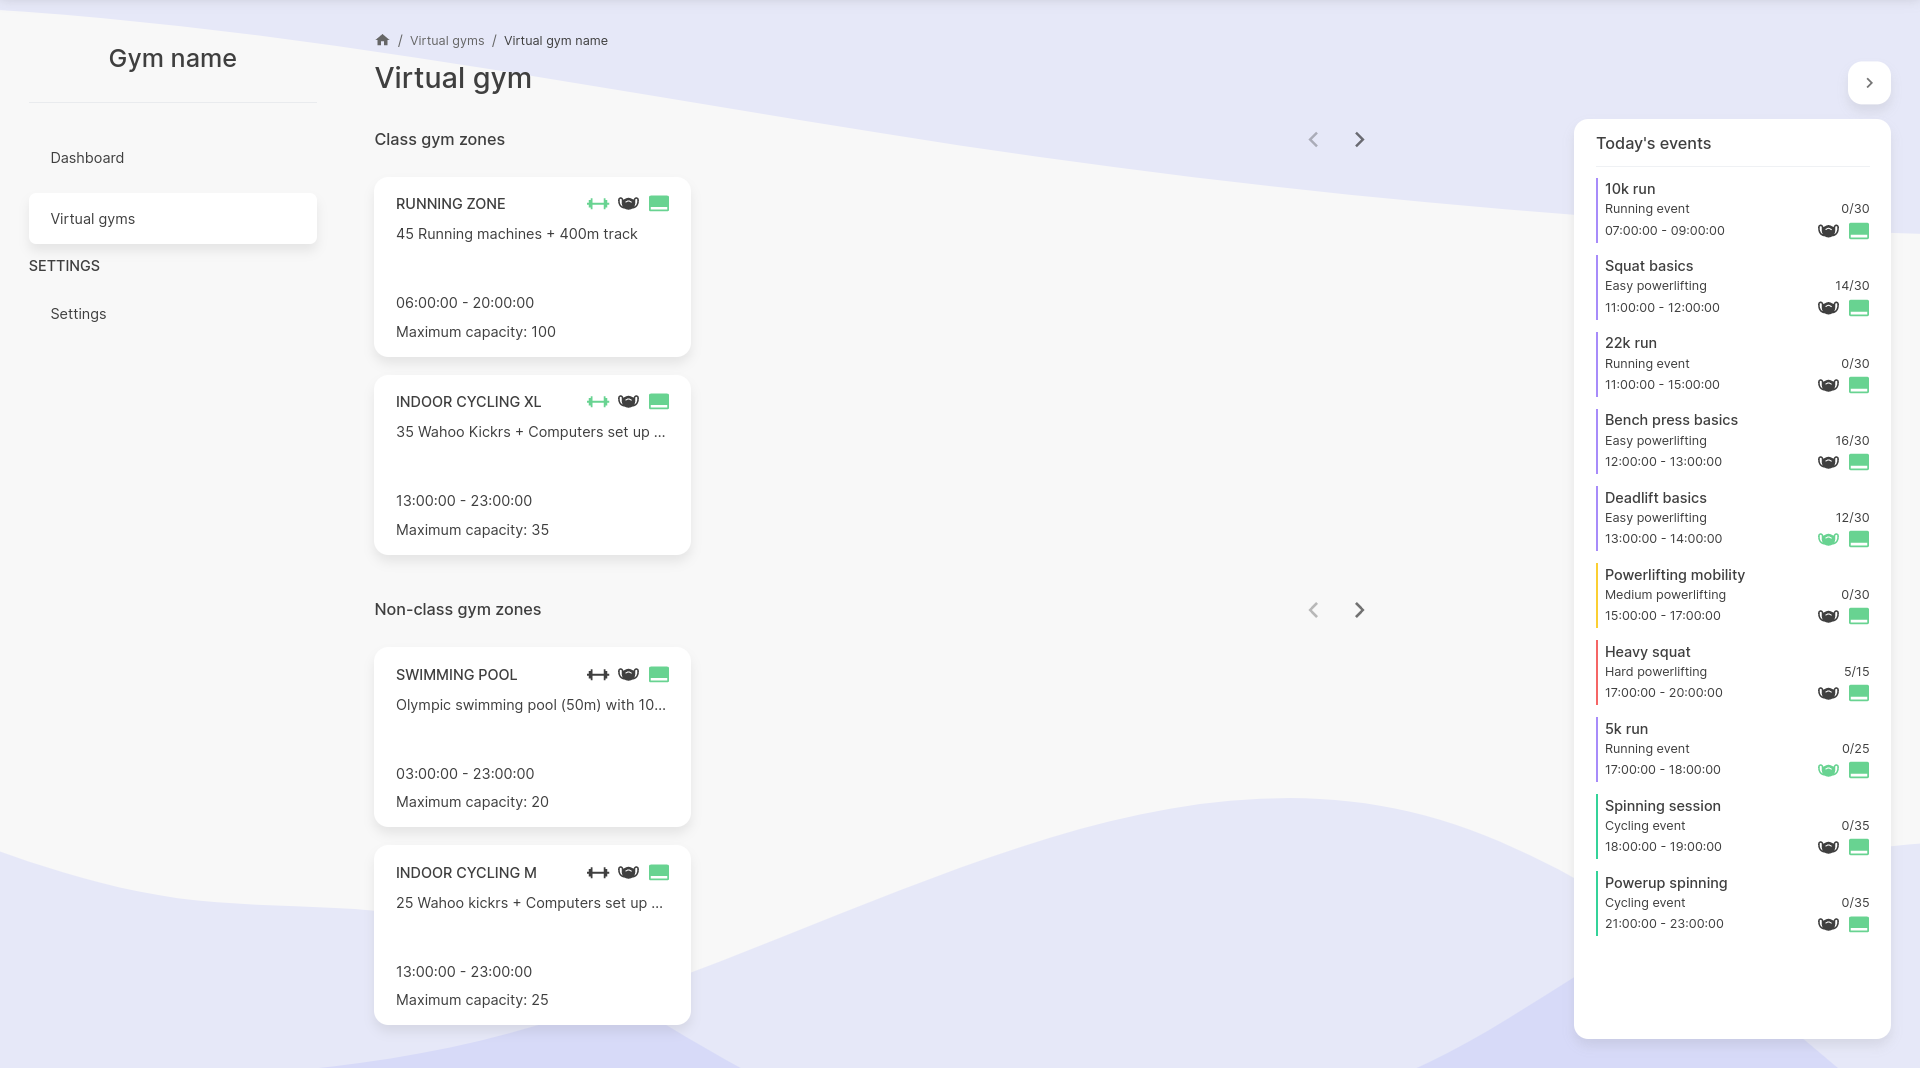
\includegraphics[width=\textwidth]{assets/client-screenshots/virtual-gym.png}
	\caption{Virtual gym page}
\end{figure}
\subsubsection{Gym zone}
\begin{figure}[H]
	\centering
	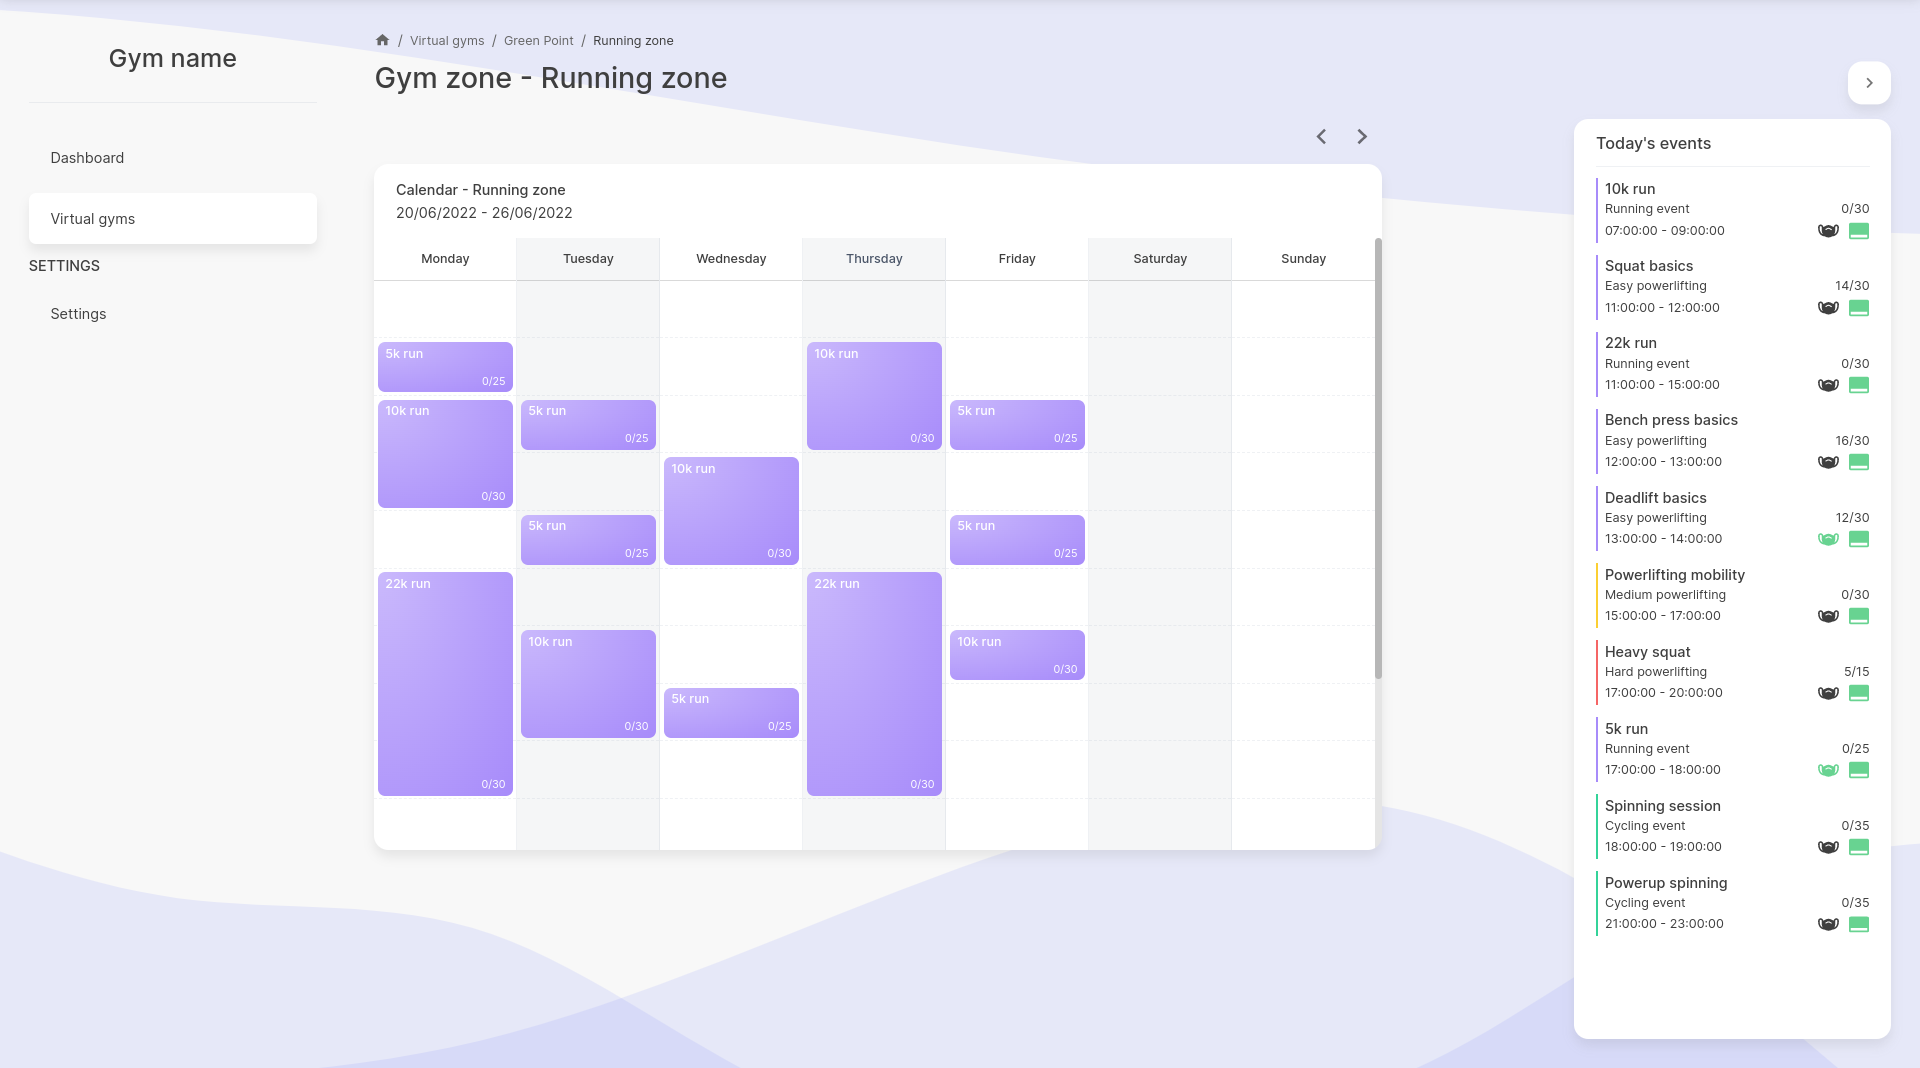
\includegraphics[width=\textwidth]{assets/client-screenshots/gym-zone.png}
	\caption{View of a gym zone}
\end{figure}
\subsubsection{Appointments}
\begin{figure}[H]
	\centering
	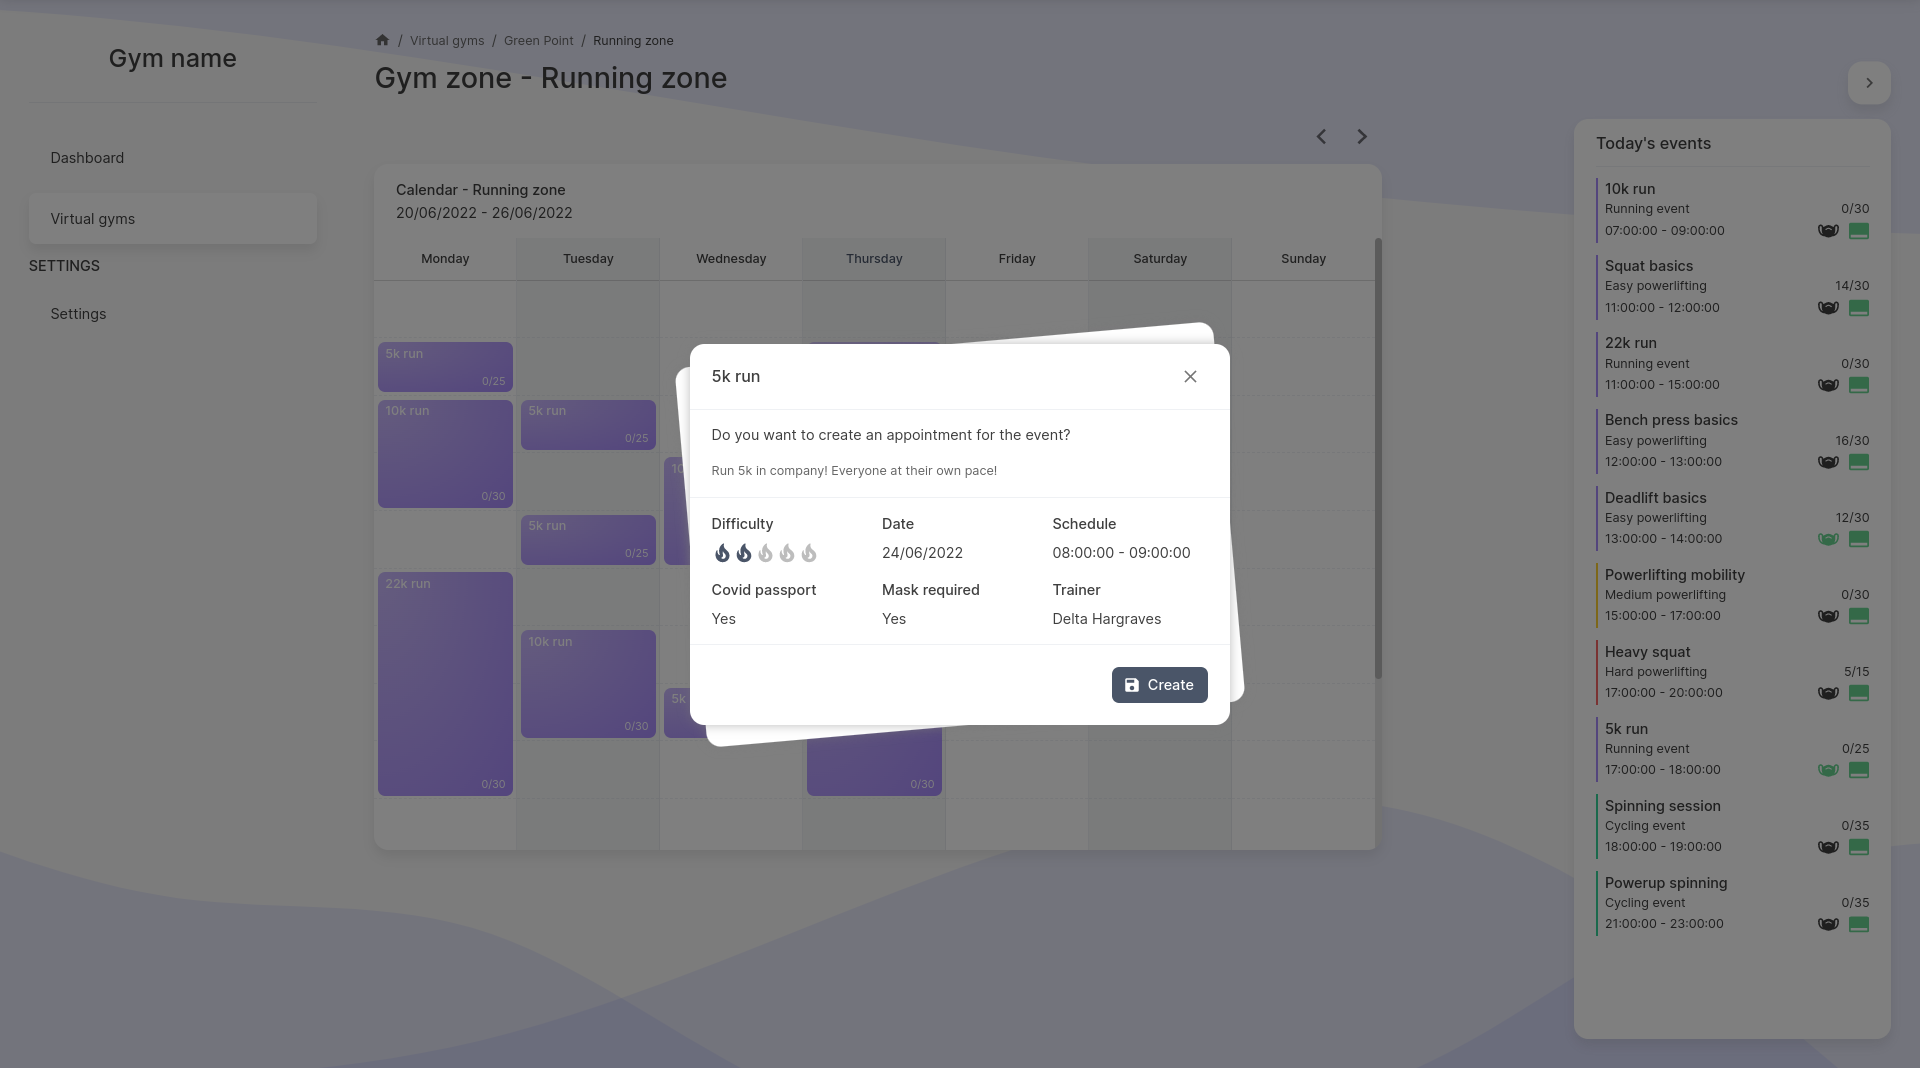
\includegraphics[width=\textwidth]{assets/client-screenshots/create-event-appointment.png}
	\caption{Creation of an appointment to an event}
\end{figure}
\begin{figure}[H]
	\centering
	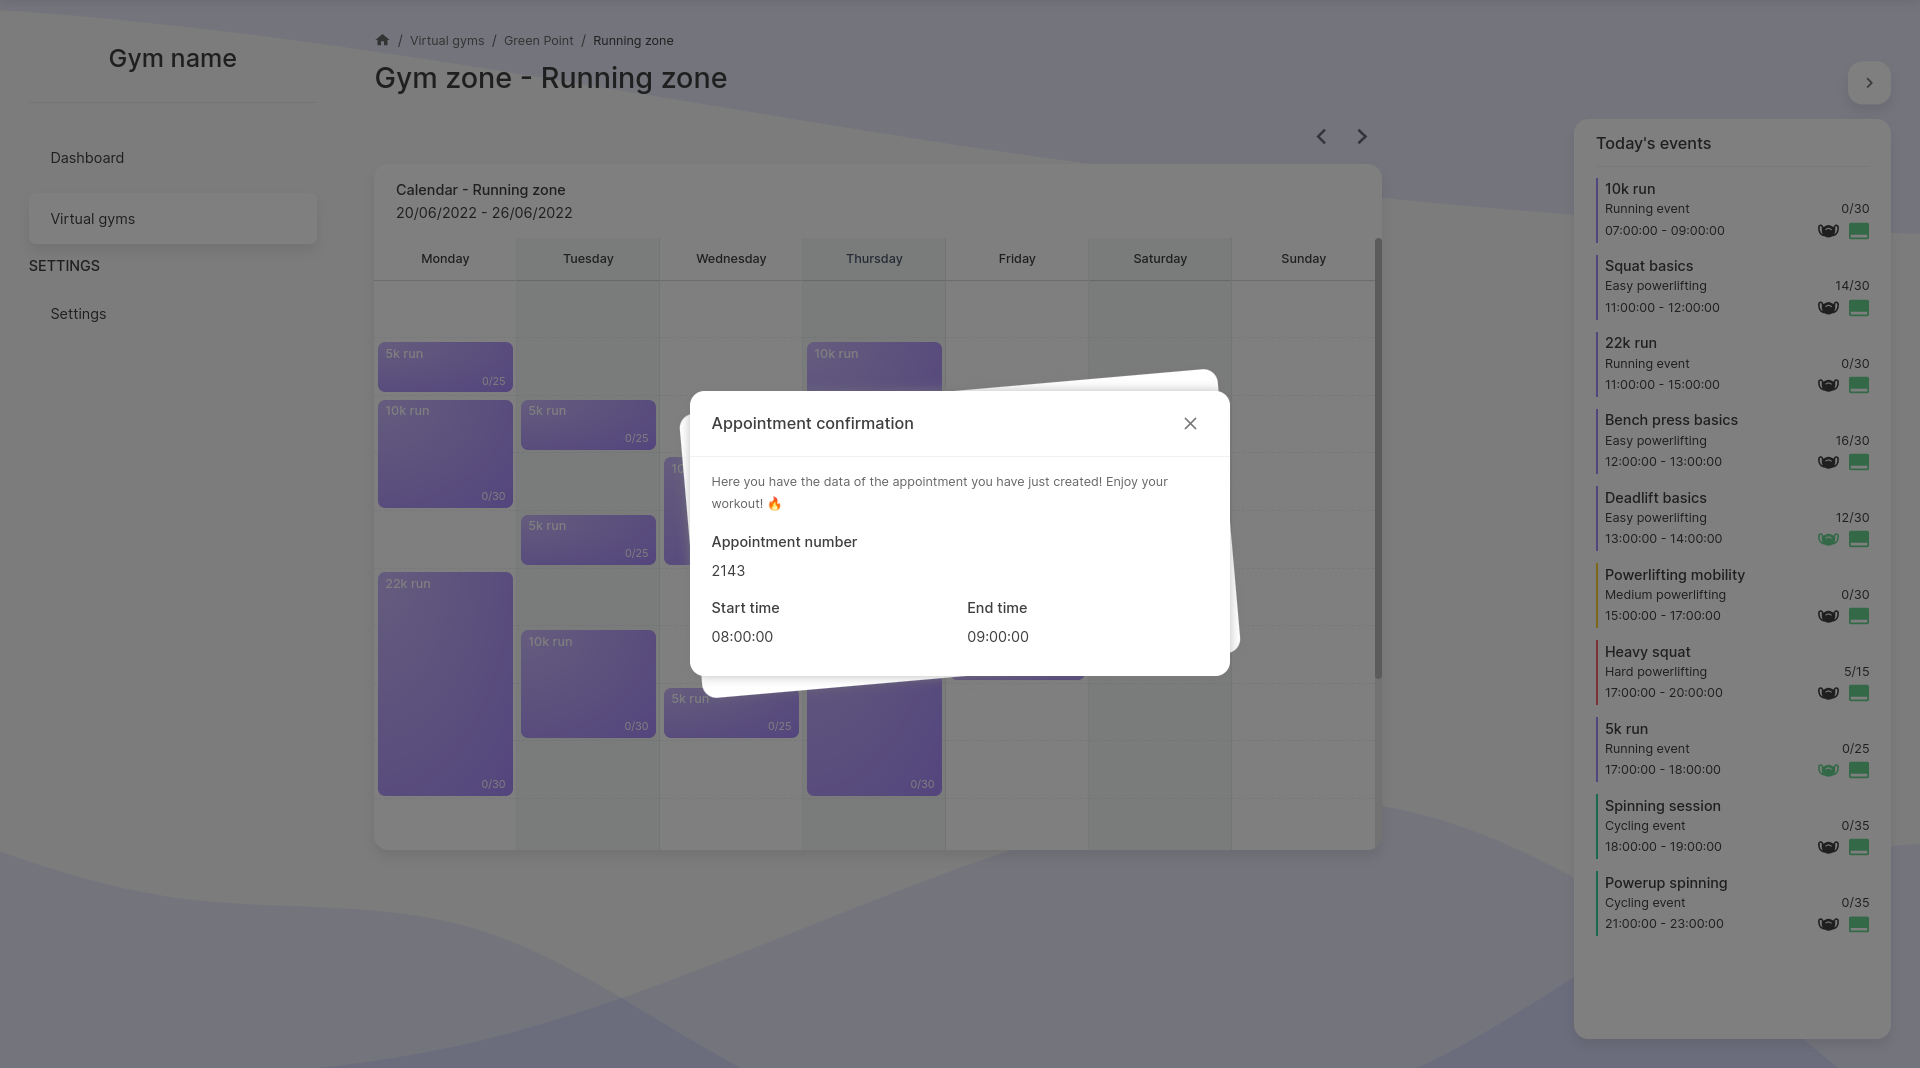
\includegraphics[width=\textwidth]{assets/client-screenshots/event-appointment-created.png}
	\caption{Confirmation of an event appointment}
\end{figure}
\begin{figure}[H]
	\centering
	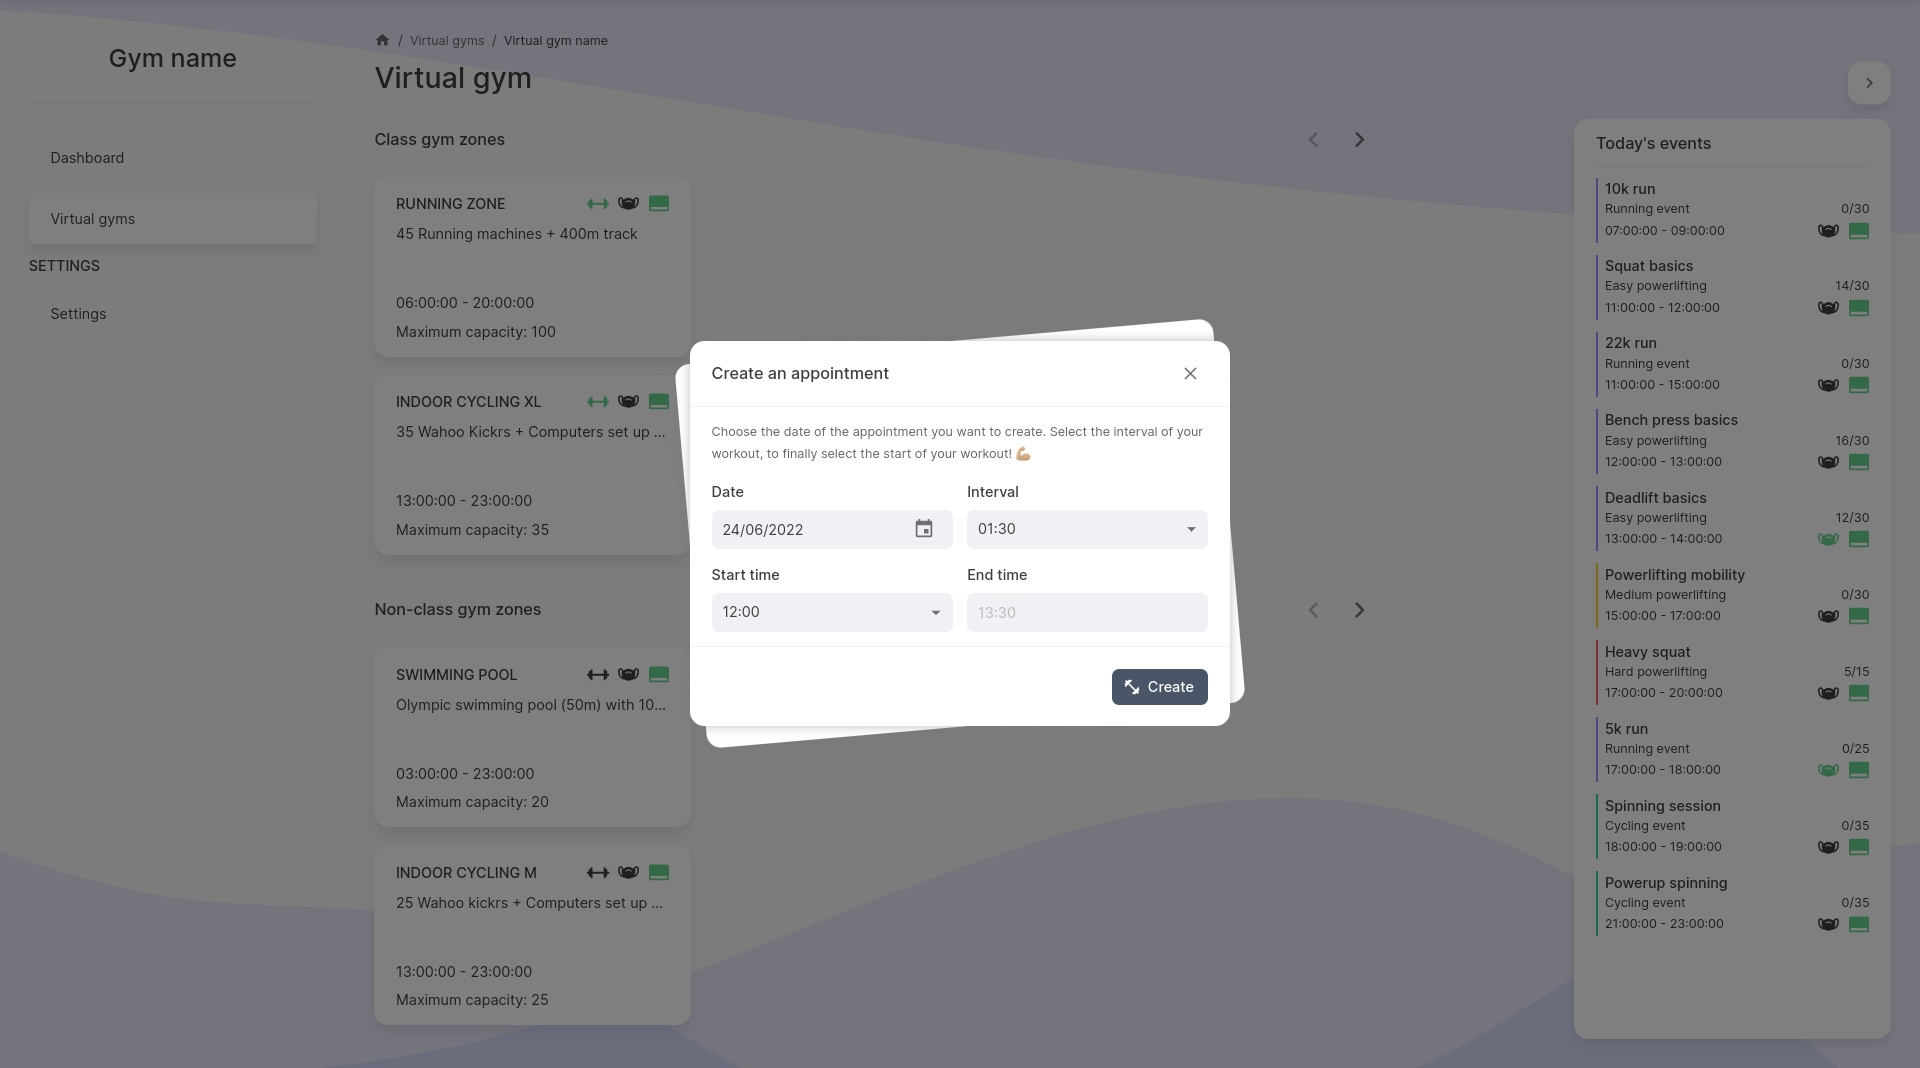
\includegraphics[width=\textwidth]{assets/client-screenshots/create-calendar-appointment.png}
	\caption{Creation of an appointment to a calendar}
\end{figure}
\begin{figure}[H]
	\centering
	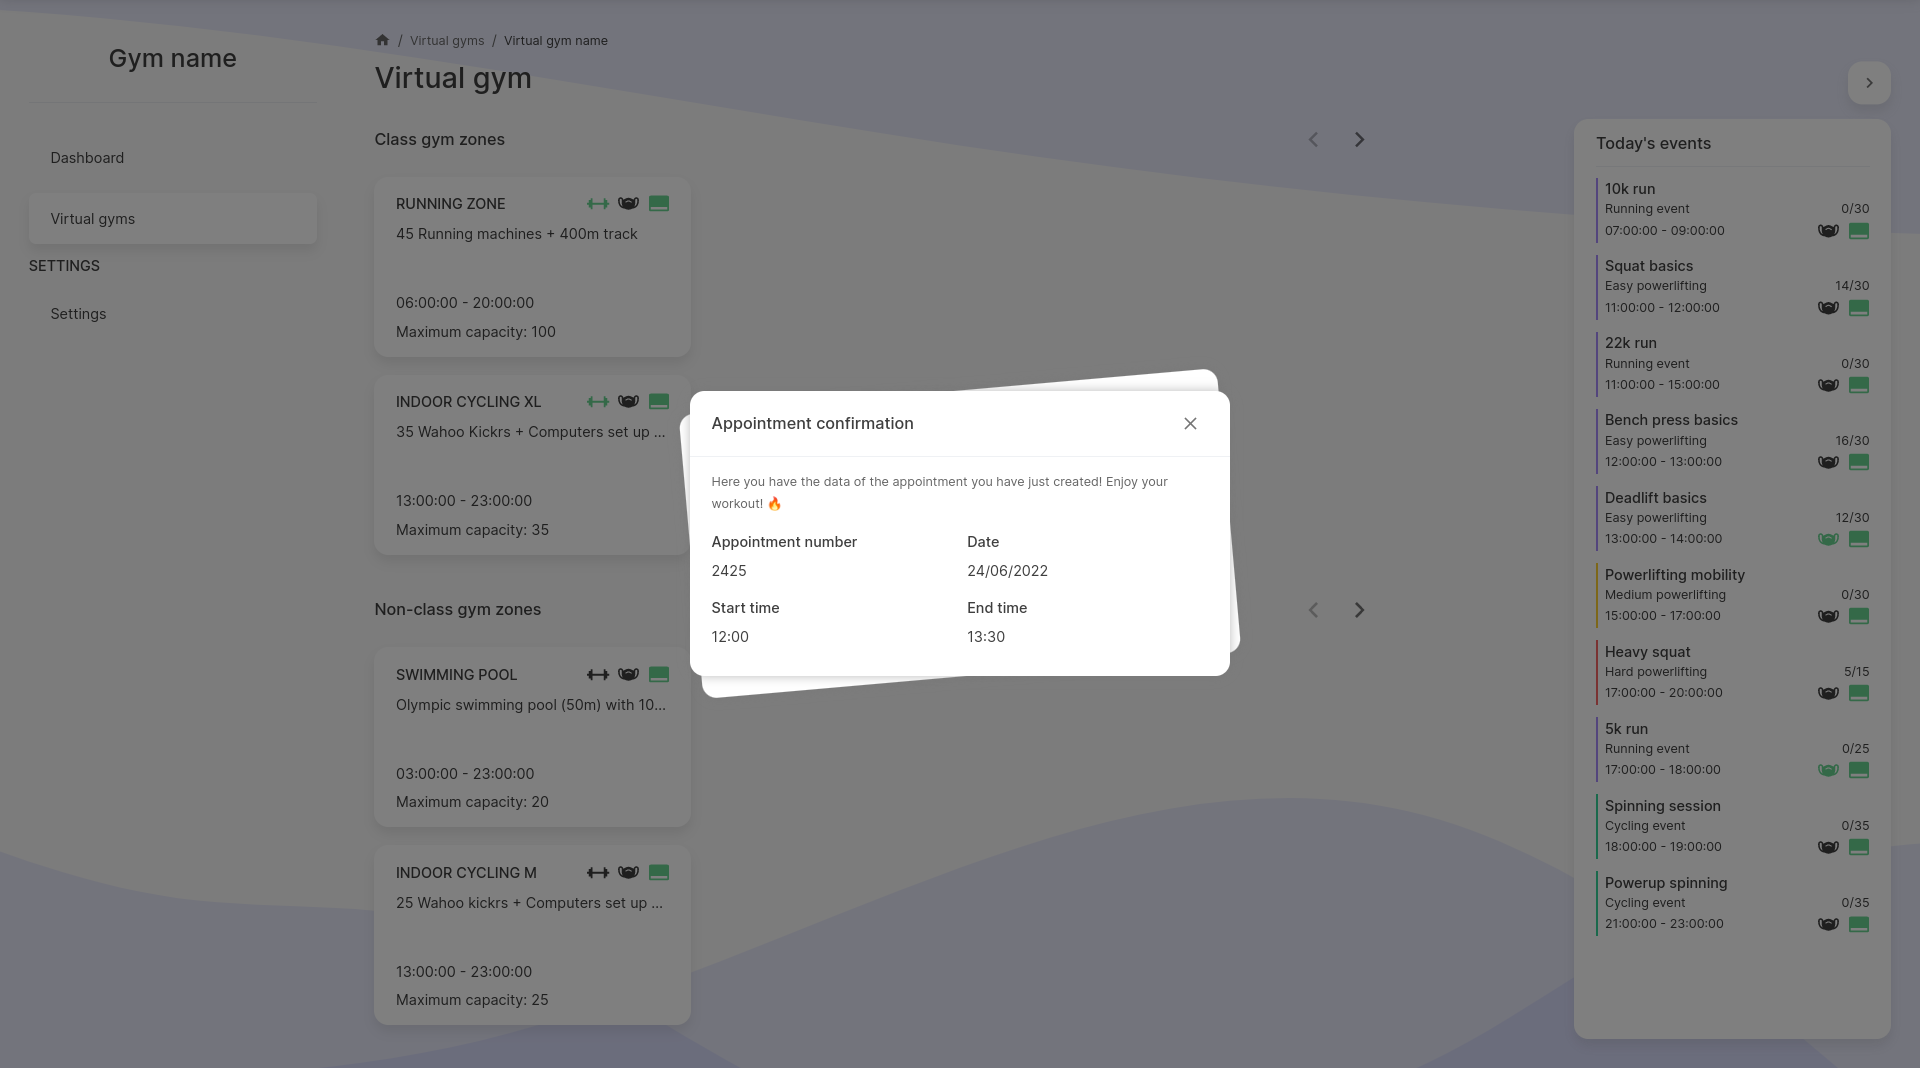
\includegraphics[width=\textwidth]{assets/client-screenshots/calendar-appointment-created.png}
	\caption{Confirmation of a calendar appointment}
\end{figure}
\subsubsection{Settings}
\begin{figure}[H]
	\centering
	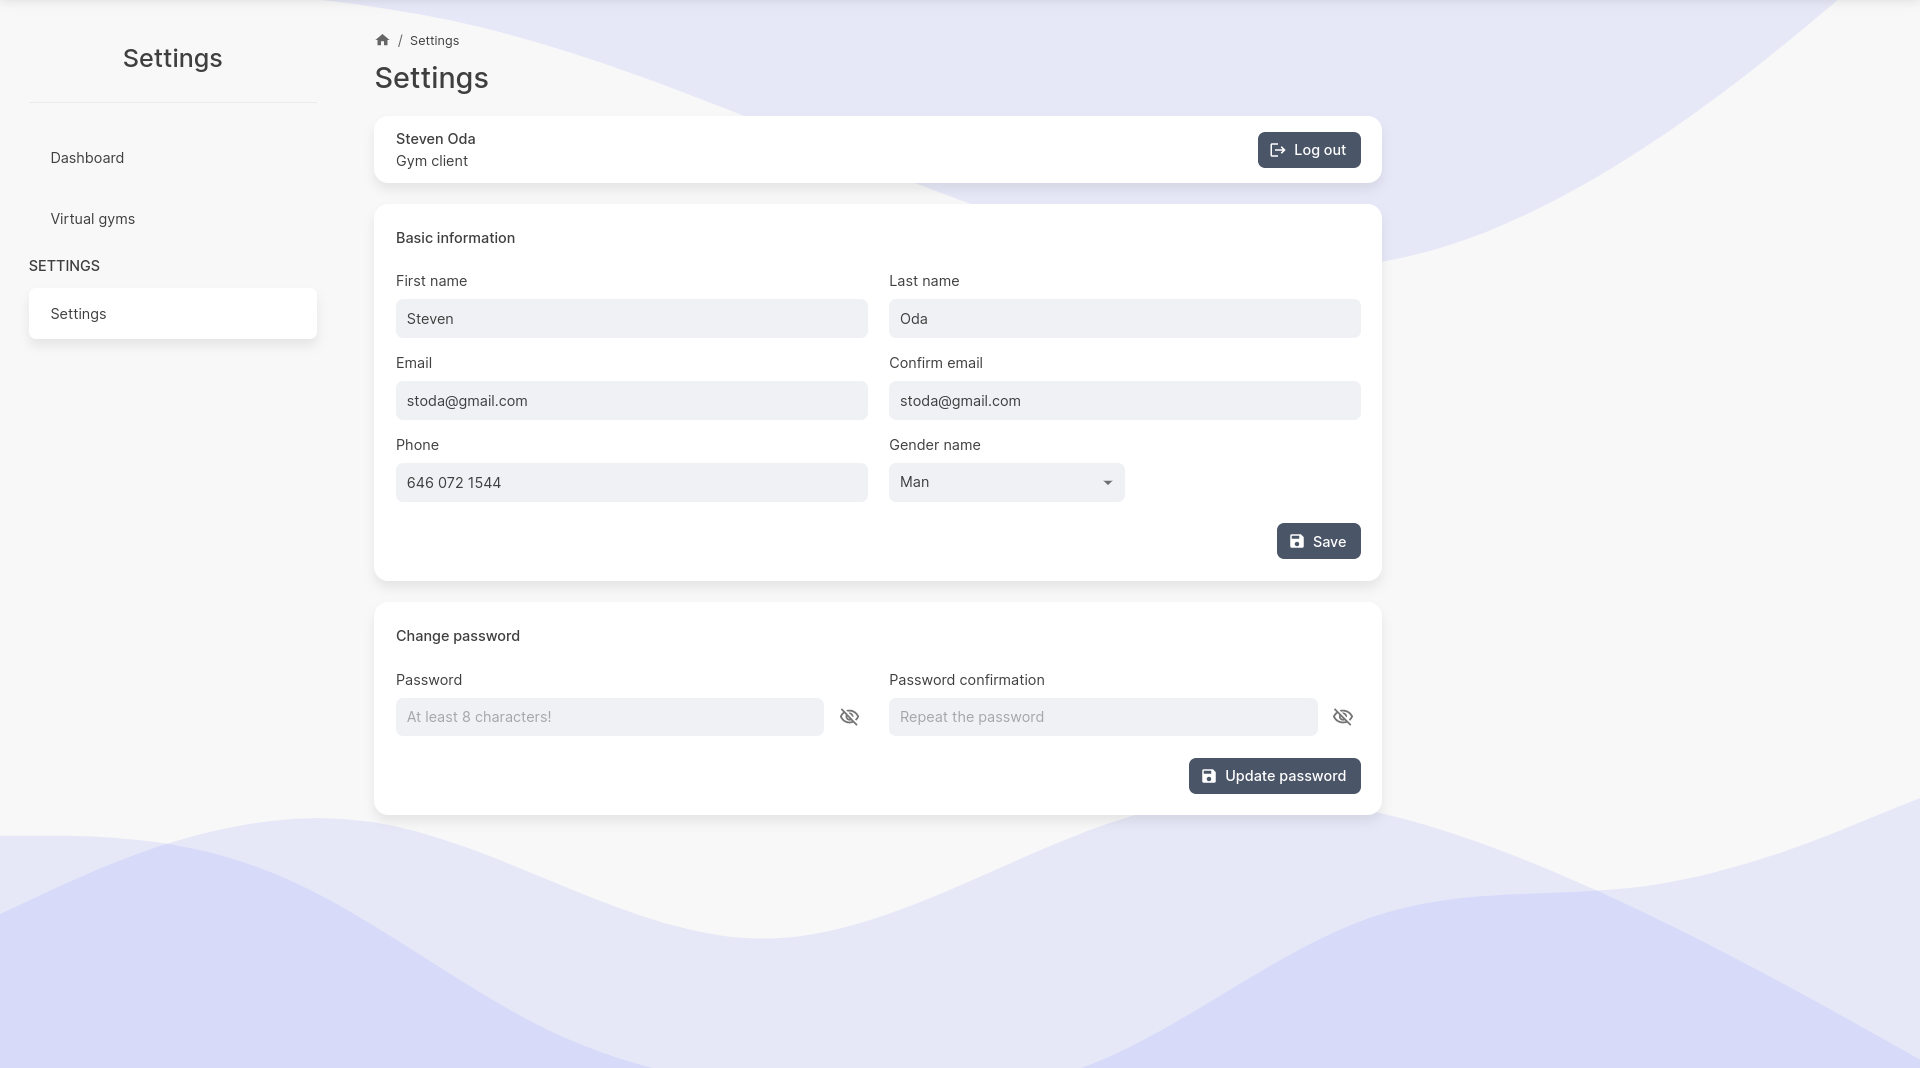
\includegraphics[width=\textwidth]{assets/client-screenshots/settings.png}
	\caption{Settings page}
\end{figure}
\end{document}